%%
%% Copyright (C) 2011 by Diane Gall <gall@spookyhill.net>
%%
%% This file may be distributed and/or modified under the conditions of
%% the LaTeX Project Public License, either version 1.3 of this license
%% or (at your option) any later version.  The latest version of this
%% license is in:
%% 
%%    http://www.latex-project.org/lppl.txt
%% 
%% and version 1.3 or later is part of all distributions of LaTeX version
%% 2003/06/01 or later.
%%
%
% York University FGS thesis/dissertation template 
%            for use with york-thesis.cls (v3.3)
%
% You really should read the documentation for the class file
% (york-thesis.pdf) to see what all of the additional macros and
% booleans do. As well, many of the macros you are used to using
% behave differently in this class. 
%
% You may, of course, remove all comments from your document.
%
\documentclass[final]{york-thesis}
\usepackage{graphicx}
\usepackage{amsmath}
\usepackage{hyperref}
\usepackage{subcaption}
\usepackage{color,soul}
\newcommand{\mathcolorbox}[2]{\colorbox{#1}{$\displaystyle #2$}}
\usepackage{float}
\graphicspath{{figures/}}

%\usepackage[letterpaper, portrait, lmargin=1.5in, rmargin=1in, tmargin=1in, bmargin=1in]{geometry}

%========== header/footer set-up  =================

\usepackage{fancyhdr}
\lhead{}
\chead{}
\rhead{}
\lfoot{}
\cfoot{\thepage}
\rfoot{}
\renewcommand{\headrulewidth}{0pt}
\renewcommand{\footrulewidth}{0pt}
\renewcommand\headheight{24pt}
\renewcommand{\baselinestretch}{1.5}
\renewcommand{\bibname}{References}


%========== citation setup  =================
\usepackage{natbib} % I use natbib, but you can use
                                % any citation format; the class file
                                % is agnostic about citation styles.            
\bibpunct{(}{)}{;}{a}{}{,}

%========= package setup ================
\setboolean{masters}{true}      % set true for a Master's thesis;
                                % false for a PhD dissertation
\setboolean{hasfigures}{true}  % set true if you have figures
\setboolean{hastables}{false}   % set true of you have tables

\title{Direct Comparisons of Polarimetric C-Band and S-Band Radar in Snow}         % this is the full title of your work
\author{Brandon M. Taylor}  % this is your name exactly as you want it
                          % to appear everywhere in your work.
\department{Earth and Space Science}   % this is the name of the programme in which
                          % you are attempting your degree 
\masterof{Science}           % this is the type of Master's degree you
                          % are attempting. If the boolean masters is
                          % false, this has no effect. 
\degreename{Master} % put the actual name of the degree you are
                          % attempting 
\date{April 2018}     % this is the month and year of defence

%========== preliminary matter =================
%
% Create these in separate files; trust me
%
% If you do not have one or more of these commands in your document,
% simply delete the line.
% 
% The following macros need appear in no particular order, but if you
% are going to use them, they have to be defined before you begin your
% document environment.
%
\abstractfile{abstract.tex}
\dedicationfile{dedication.tex}
\acknowledgementsfile{acknowledgements.tex}
%\prefacefile{preface.tex}
%
% Your committee members list has to be an enumerated list.
%
\committeememberslist{
  \begin{enumerate}
    \item Mark Gordon
    \item George Isaac
    \item Dave Sills
    \item Don Hastie
  \end{enumerate}}

%============ document begins ==================
%

\begin{document}
\makefrontmatter

%
%   the include commands for chapters go here
%

\chapter{Chapter One}
\section{Introduction}
Weather radar is an invaluable tool for nowcasting severe weather. In Canada, lake-effect snows are a severe weather event which have big impacts on a large
sector of the population. While the current Canadian C-Band radar systems have been proven in this regard, there is uncertainty with whats to come with the
new S-Band systems. While no prototype system is available to test in the Great Lakes area, the next best stand-in to compare with are the current S-Band
radars in the United States. King City radar (CWKR) has been compared with the Buffalo, NY radar (KBUF) previously by \cite{Boodoo2015}, but this case was
for rainfall. Furthermore, C-Band radars have been compared with S-band radars before by \cite{Abon2014}, but polarimetric variables weren't considered. To
compare the two radars, the data will be objectively analyzed. Radar data objective analysis is most prominently used in created mosaics of multiple radars
for projects such as the Multi-Radar Multi-Sensor project by NSSL \citep{Zhang2016}. It is also used extensively for research purposes, including studying
snow squalls \citep{Mulholland2017}.  The goal of this study is to show that there will be no loss in quality of radar observations for the purposes of
nowcasting lake-effect snow with S-Band radar. Another goal is to directly compare polarimetric moments, which has not been done in this manner before, and
identify any biases. It is important to remove biases as no amount of spatial or temporal smoothing will remove them. With bias-adjusted values from two independent sources, a high-confidence conclusion can be made on the types of hydrometeors present in the common sampling volumes. Although dual-pol radar has matured within the research community, operational deployment has been a much slower process. Many studies have been undertaken in regards to quantitative precipitation estimation using dual-pol variables for rainfall, but studies involving snow have been much more limited. Findings here should increase confidence in comparing dual-polarmetric at two different wavelengths, and demonstration the information rich nature of these variables. 
\section{Background}
First, it is important to provide some background on the weather radar moments that are presented in this study, from both single and dual polarized signals.
The convention for representing these moments symbolically hereafter is lower-case subscript for linear units and upper-case subscript for logarithmic units,
i.e. $Z_{DR}$ is logarithmic while $Z_{dr}$ is linear.
\subsection{Radar Locations}
In Canada, there is one active C-band weather radar with dual-pol capabilities. It is located north of Toronto, in King City, while the rest of the network is
currently undergoing an upgrade to polarimetric S-Band. Its neighbor to the south, KBUF, was upgraded to dual-pol in 2012 as part of a network wide upgrade. 
\begin{figure}[h]
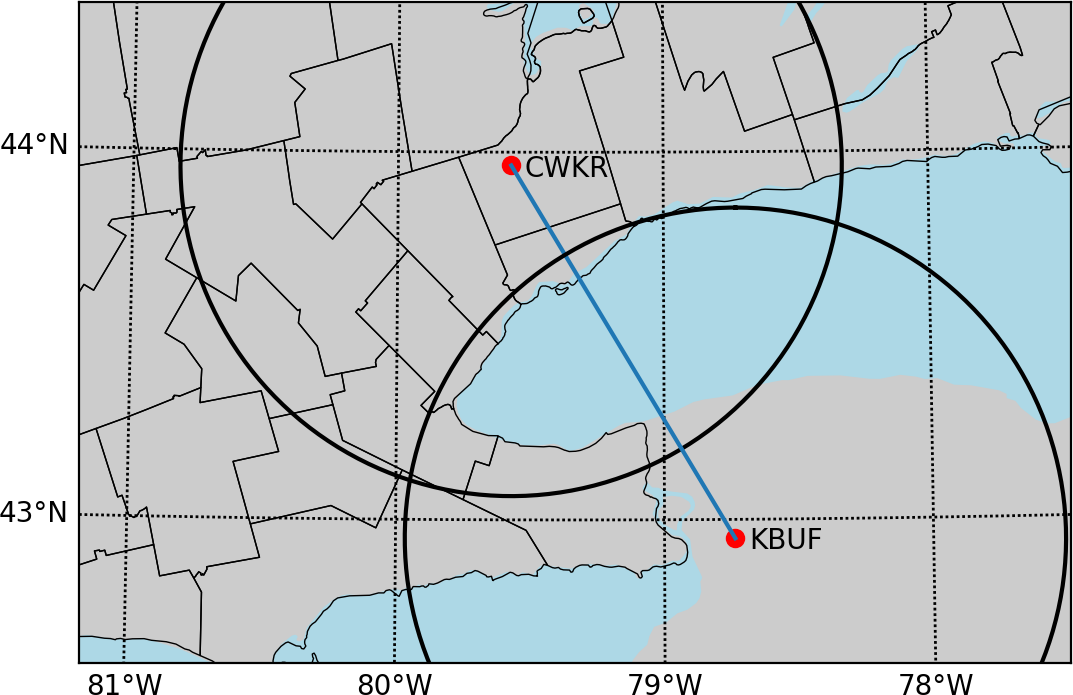
\includegraphics[width=\textwidth]{map}
\caption{The location of the NWS Buffalo Radar (KBUF) and King City Radar (CWKR) are shown as red dots, with a 100 km range ring around each. The distance
between the two, drawn as a blue line, is 131.5 km.} 
\label{map}
\end{figure}
Figure \ref{map} shows the geographic location of the radar sites in comparison with each other.
\subsection{Reflectivity Factor ($Z_{h}$)}
The foremost moment derived from radar is the reflectivity factor ($Z_{h}$), where the
subscript denotes its derivation from the horizontally polarized signal. This variable
measures the number density $N(D)$ of hydrometeors of diameter $D$ per unit volume, as
presented in Equation \ref{eq:ref_factor}. Due to uncertainties about what type of
target is actually doing the scattering, it is typically represented as the equivalent
reflectivity factor $Z_{eh}$, where $Z_{h}$ = $Z_{eh}$ if the targets are made of liquid 
water and are comparatively small to the wavelength \citep{Fabry2015}. The two names are 
essentially interchangeable, but the nomenclature $Z_{eh}$ will be used in this study to 
acknowledge the presence of non-ideal targets, e.g. snow crystals.
\begin{equation}\label{eq:ref_factor}
Z_{h} = \int_0^{\infty} N(D)D^6dD \ (mm^6/m^3)
\end{equation}
\subsection{Differential Reflectivity ($Z_{dr}$)}
Radars equipped with dual-polarimetric (dual-pol) capabilities are still an emerging technology, in terms of operational meteorological applications. These
types of radar systems are capable of transmitting and receiving two orthogonally polarized electromagnetic waves in order to deduce more information about
the microphysical structure of hydrometeors. One of the main variables this allows them to produce is $Z_{DR}$, defined as the ratio of the horizontal
channel reflectivity ($Z_H$) to the vertical channel reflectivity $Z_{V}$). This can be simplified to the difference between the two using the logarithmic
quotient rule, since they are represented in logarithmic units. Equation \ref{eq:zdr} demonstrates this concept.
\begin{equation}\label{eq:zdr}
Z_{dr} = 10 * \log_{10}(\frac{Z_H}{Z_V}) = Z_h - Z_v
\end{equation}
\subsubsection{Interpretations of $Z_{DR}$ in Snow}
In snowfall, $Z_{DR}$ can be a powerful tool for deducing the predominant crystal habit and type. Values of $Z_{DR}$ typically observed for dry aggregated snow at cold temperatures range from $0 < Z_{DR} < 0.2$ dB, while pristine ice crystals and lightly aggregated crystals range from $0.4 < Z_{DR} < 3$ dB, both for a range of $Z_{eH}$ of $5 < Z_{eH} < 30$ dBZ. Figure \ref{zdr_chart} shows expected $Z_{DR}$ for frozen and liquid hydrometeors, as well as non-meteorological targets. In this study, we are only concerned with hydrometeors that are sufficiently frozen.
\begin{figure}[H]
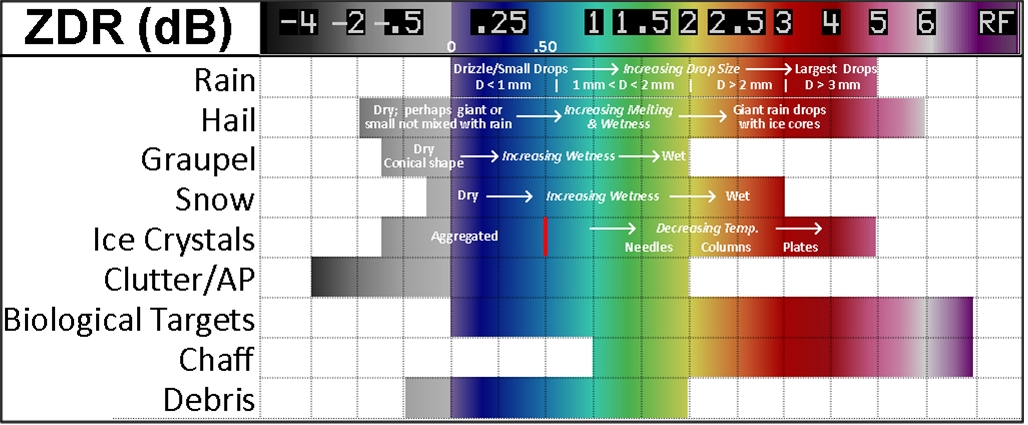
\includegraphics[width=\textwidth]{zdr_chart}
\caption{Chart of expected ranges of $Z_{DR}$ for a variety of targets. Taken from \citet{Fabry2015}.} 
\label{zdr_chart}
\end{figure}
\subsection{Co-polar Cross-Correlation Coefficient ($\rho_{hv}$)}
With the advent of Simultaneous Transmit and Receive (STAR) radar systems, which both radars used here have, it is possible to perform the zero time-lag
cross-correlation between the time series data obtained from horizontal and vertical channels. This is known as the Co-polar Cross-Correlation Coefficient
($\rho_{hv}$) in radar meteorology, and ranges from 0 to 1. Low values indicate pulse volumes containing heterogeneities, while a value of 1 indicates
matching, homogenous volumes. For an ensemble of scatters, Equation \ref{eq:backscatter} defines the backscattering matrix used in the definition of
$\rho_{hv}$ in Equation \ref{eq:rhohv}, as defined by \citet{Ryzhkov2007b}.
\begin{equation}\label{eq:backscatter}
\mathbf{S} = \begin{bmatrix}
             S_{hh}       & S_{hv} \\
             S_{hv}       & S_{vv} \\
             \end{bmatrix}
\end{equation}
\begin{equation}\label{eq:rhohv}
\rho_{hv} = \frac{\langle{S_{vv}{S_{hh}}^{*}\rangle}}{\sqrt{\langle{{S_{hh}}^{2}\rangle}\langle{{S_{vv}}^{2}\rangle}}}
\end{equation}
\subsubsection{Interpretations of $\rho_{hv}$ in Snow}
Contamination from clutter and other non-meteorological targets can be filtered by using a $\rho_{hv}$ threshold of 0.95, as suggested by \citet{Straka2000}.
Using this threshold can also be used to avoid Mie scatters, which becomes a bigger problem at C-Band wavelengths \citet{Fabry2015}.
 




\chapter{Chapter Two}
\section{Methodology}
\subsection{Comparison of Radar Systems}
Comparing two radar datasets is fraught with challenges; solutions to meet this challenge are presented herein. Even though the radar system characteristics
are not identical, the measurements are comparable due to the design of the weather radar equation, which accounts for the sensitivity of the radar system
itself \citep{Rogers1989}. The area of study was chosen to ensure that the coinciding radar scans had similiar resolution samples and beam heights. 
\begin{figure}[h]
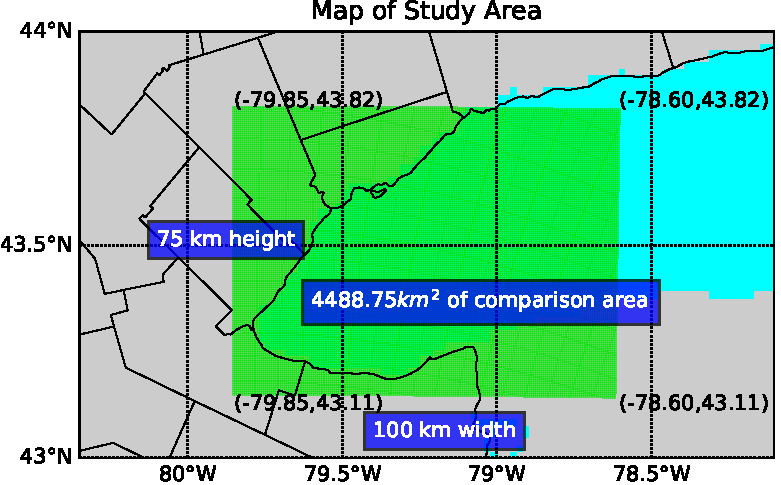
\includegraphics[]{study_area}\centering
\caption{Bounding box of the study area, denoted by the green shading.} 
\label{fig:study_area}
\end{figure}
Lake Ontario happens to be the perfect area to bound between the radars, therefore only data from areas over water inside the bounding box depicted in Figure
\ref{fig:study_area} are used. This also ensures that no ground clutter is incorporated into the analyses.
\subsubsection{Comparing Radar Characteristics}

As presented in Equation \ref{eq:weather_eq}, the weather radar equation is defined by constant parameters dependent on the radar system characteristics, and
varying properties related to the target. This equations determines the theoretical mean power ($\bar{P_r}$) that should be returned to the radar receiver.
\begin{equation}\label{eq:weather_eq}
\bar{P_r} = \frac{\pi^3c}{1024 \ln(2)} \Bigg[\frac{P_t \tau G^2 \theta^2}{\lambda^2}\Bigg]_{dBZ_0} \Bigg[\mathcolorbox{yellow} {||K_{w}||^{2}}\frac{Z_{eh}}{r^2}\Bigg]_{TARGET}
\end{equation}
The target properties are dielectric constant (K), range (r) and equivalent reflectivity factor $Z_{eH}$. Conversely, the radar parameters ideally remain
unchanged from their values upon installation of the radar system. These parameters form the radar constant, symbolically expressed as $dBZ_0$. The
parameters that define this constant include the power transmitted ($P_t$), the pulse length ($\tau$), the antenna gain (G), the angular beamwidth
($\theta$), and the wavelength ($\lambda$).
\begin{equation}\label{eq:radpow}
\mathcolorbox{yellow}{Z_{eH}} = 10 \log{\bar{P_r}} + 20 \log r - dBZ_0
\end{equation}
Equation \ref{eq:radpow} shows how $dBZ_0$ is subtracted out from the full calculation of $Z$. This means that values from two different systems are comparable, as the contributions to the returned power intrinsic to the radar are negated. Next, Table \ref{radarspecs} compares parameters for both
radar systems. The biggest difference between the two is the wavelength, with CWKR operating in the C frequency band and KBUF operating in the S frequency
band. It should be noted that although KBUF has a larger physical beamwidth than CWKR, it achieves an effective azimuthal resolution of $0.5^{\circ}$ through
an over-sampled data windowing technique \citep{Torres2007}. Therefore, the two radars are matched in azimuthal resolution, while CWKR has twice the range
resolution of KBUF. Also, it should be stated that the signal processors used in both radar systems are in the
Vaisala SIGMET series, therefore they measure
$Z_{eH}$ and $Z_{DR}$ using 8 bit resolution. For $Z_{eH}$, the data intervals of -31.5 dBZ to +95.5 dBZ yield a
data resolution of 0.5 dBZ.  For $Z_{DR}$, an interval of -7.94 dB to +7.94 dB yields a resolution of 0.0625 dB.

\begin{table}[h]
    \caption{Specifications of each radars system, with symbols as used in Eq. \ref{eq:radpow}. Pulse Length is specified as short pulse/long pulse}\label{radarspecs}
    \begin{center}
    \begin{tabular}{|l|c|c|c|}
    \hline
     field [symbol](unit) & King City (CWKR) & Buffalo (KBUF) & New CWRN \\
    \hline\hline
    Wavelength [$\lambda$](cm) & 5.6  & 10.7 & 10.6\\
    \hline
    Beamwidth [$\theta$] ($^\circ$)  & 0.62  & 0.92 & 0.88 \\
    \hline
     Antenna Gain [G] (dB) & 45.5 & 49.2 & 45.8\\
    \hline
     Peak Power (kW) & 250 & 1000 & 1000 \\
    \hline
     Pulse Length [$\tau$] ($\mu s$) &  0.8/2.0 & 1.5/4.5 & 0.4/4.5 \\
    \hline
     Lowest Elevation Angle ($^\circ$) & 0.2 & 0.5 & 0.4 \\
    \hline
     Range Resolution [$r$] (m)& 125 & 250 & 500 \\
    \hline
    \end{tabular}
    \end{center}
\end{table}


\subsection{Distance-Weighting Scheme}
The biggest challenge when comparing radar resolution volumes measured by radars that are not co-located is resolving the differences in coordinate system. A
resolution volume is defined as volume irradiated by the idealized Gaussian beam pattern for each range gate, otherwise known as a bin. Resolution volumes
are sampled natively in the spherical coordinate system; although there may be some overlap, the shape of the bins will vary drastically. Differences between
KBUF and CWKR bin geometry can be ascertained from Figure \ref{fig:compare_bins}. 
These differences require the radar data to be objectively analyzed onto a common coordinate system, which can be achieved through a distance-weighting
scheme. This method was adopted in the open source software module called the Python ARM Radar Toolkit (Py-ART) \citep{Py-ART}, which is used here. In
accordance with the recommendations of \cite{Pauly1990}, a grid resolution ($\Delta x$, $\Delta y$) of 500 meters is chosen.A Barnes distance-weighting scheme is used for this analysis. 
\begin{equation}\label{eq:barnesdws}
f^{'}_{p} = \sum_{b=1}^n  e^{-(d_b/\kappa)^{2}} f_q  \bigg/ \sum_{b=1}^n e^{-(d_b/\kappa)^{2}}
\end{equation}
The Gaussian weighting function used in said scheme is given in Equation \ref{eq:barnesdws}. It shows that the value of the analysis at some point $p$ is
equal to sum of weights convolved with the actual values at bin $b$ in radar space, divided by the sum of the weights. The summation is performed over $n$
number of bins that are within the radius of influence ($\kappa$) of the center point of the grid cell, and $d_{b}$ is is the horizontal distance from the native
bin to the center point of the cell. Vertical distance is neglected, as only the lowest elevation angle from the radars are included for comparison.
\begin{equation}\label{eq:roi}
\kappa = d_{0} * \tan{\theta}
\end{equation}
The definition of $\kappa$ is found in Equation \ref{eq:roi}, where $d_{0}$ is the horizontal distance from the grid cell to the radar and $\theta$ is the angular\
beamwidth. This completes the framework for comparing the radar datasets in this study.
\begin{figure}[t!]
\centering
   \begin{subfigure}{1.0\textwidth} \centering
     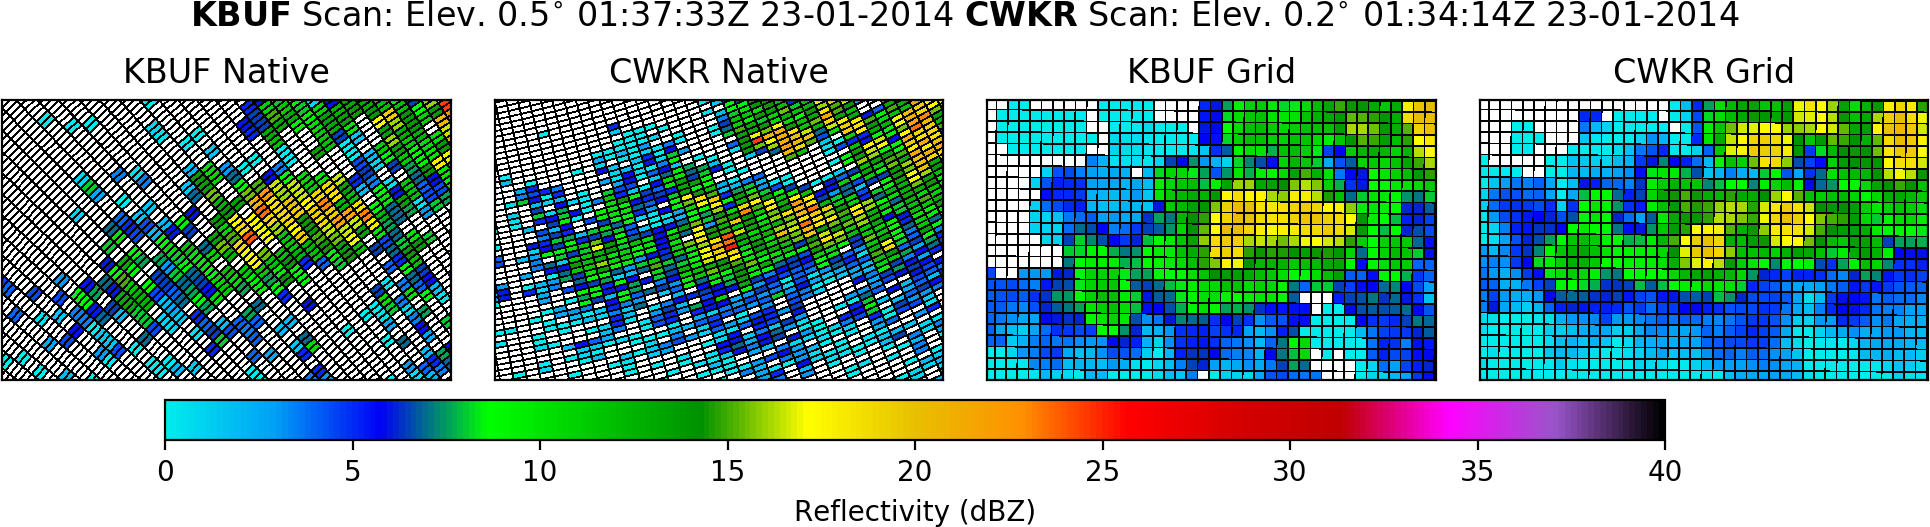
\includegraphics[width=1\linewidth]{compare_bins_ref}
     \caption{$Z_H$ comparison, shows the transformation from a smooth input to smooth gridded output.}\label{fig:compare_ref}
   \end{subfigure}
   \begin{subfigure}{1.0\textwidth} \centering
     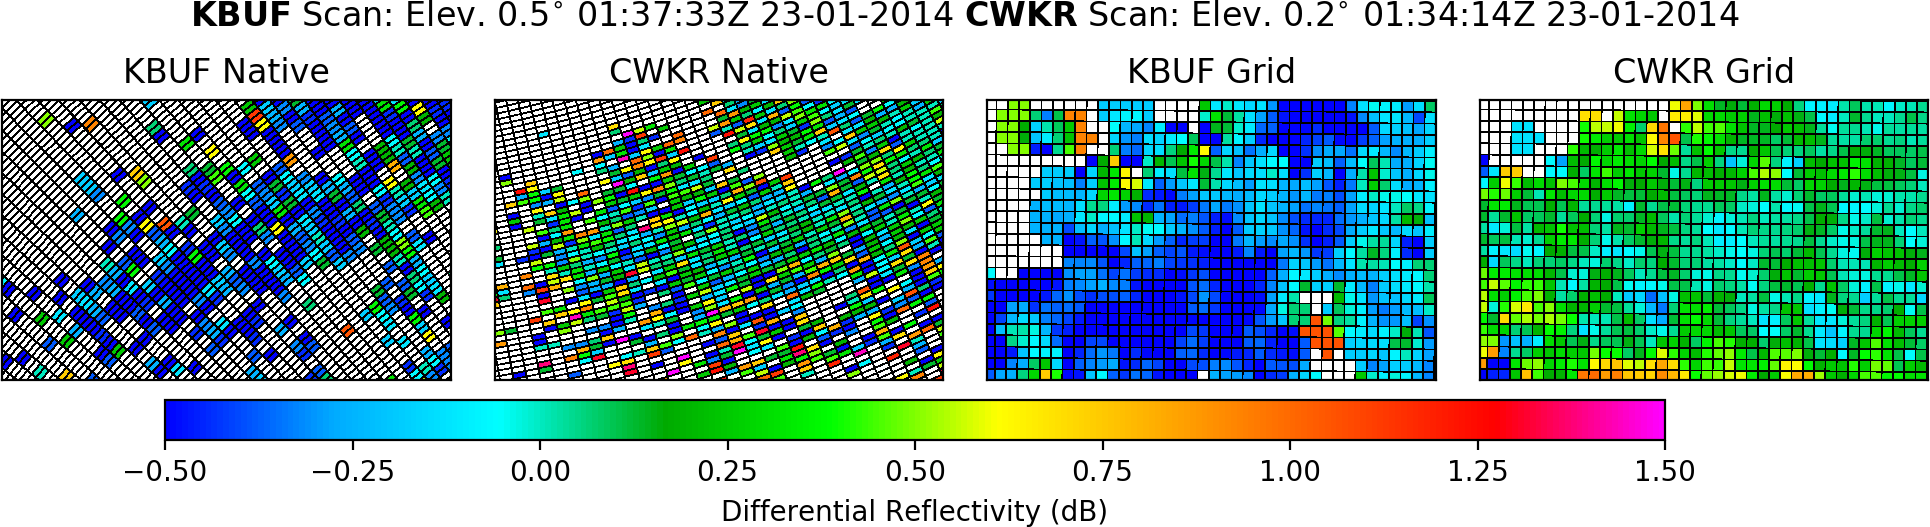
\includegraphics[width=1\linewidth]{compare_bins_zdr}
     \caption{$Z_{DR}$ comparison, in contrast with (a), shows the limitations of representing an non-linear field with an isotropic distance-weighting
     function. }\label{fig:compare_zdr}
   \end{subfigure}
\caption{Base moment comparisons between radars over Lake Ontario, with dimensions of 20x12.5 km. Left panels are in native radars coordinates, with gates
outlined in black. Right panels are transformed to a common Cartesian grid, with grid cells outlined in black.} \label{fig:compare_bins}
\end{figure}

\section{Selection of Cases}
Cases selected for this study were chosen entirely based on the pattern of motion and banding of the radar
echoes. Radar mosaics for the study area were
manually examined, beginning in 2014. When time intervals with echoes in the study area were observed, it was
noted whether they moved repeatedly over the same area,
or were progressive.  Also, it was noted whether they exibited meso-$\beta$ length scales ($\sim$ 20 km wide),
or synoptic length scales ($>$ 200 km) \citep{Orlanski1975}. The narrow bands that moved over the same area
were classified as lake-effect driven events, while the progressive, wide-areas of precipitation are classified as
synoptically driven events. A tabulation of important level temperatures for the five lake-effect snow events selected
is shown in Table \ref{eventslake}, along with the time interval during which radar scans were chosen. Synoptic
events are given in Table \ref{synopticevents}. This indicates that all events were sufficiently below freezing, and
dry snow/ice crystals were the predominant hydrometeor type.

\begin{table}[H]
    \caption{Temperatures at two important levels from radiosonde launched closest in time to the selected lake-effect snow events, with the time interval during which radar scans were chosen.}\label{eventslake}
    \begin{center}
    \begin{tabular}{|l|c|c|c|}
    \hline
     BUF - Radiosonde & Radar Times & 850mb T ($^{\circ}C$) & Sfc. T ($^{\circ}C$)\\
    \hline\hline
    2014-01-23 00Z & 0100-1000Z & -22.5 & -14.9 \\
    \hline
    2015-01-06 12Z & 1200-1700Z & -20.1 & -11.7 \\
    \hline
    2015-02-14 12Z & 1000-1400Z & -14.9 & -6.9 \\
    \hline
    2015-02-18 12Z & 2100-2359Z & -17.3 & -10.1 \\
    \hline
    2016-02-10 12Z & 1300-2359Z & -10.5 & -2.7 \\
    \hline
    \end{tabular}
    \end{center}
\end{table}

\begin{table}[H]
    \caption{Temperatures at two important levels from radiosonde launched closest in time to the selected synoptic snow events, with the time interval during which radar scans were chosen.}\label{synopticevents}
    \begin{center}
    \begin{tabular}{|l|c|c|c|}
    \hline
     KBUF - Radiosonde & Radar Times & 850mb T ($^{\circ}C$) & Sfc. T ($^{\circ}C$)\\
    \hline\hline
    2014-01-18 12Z & 0600-0800Z & -11.3 & -6.5 \\
    \hline
    2014-02-01 12Z & 1500-1800Z & -4.7 & -3.1 \\
    \hline
    2015-01-07 12Z & 0900-1100Z & -19.5 & -10.1 \\
    \hline
    2015-02-06 12Z & 0900-1030Z & -16.3 & -10.7 \\
    \hline
    2016-12-15 12Z & 0920-1020Z & -20.3 & -12.3 \\
    \hline
    \end{tabular}
    \end{center}
\end{table}
\section{Filtering Conditions}
Several conditions were used to narrow down the selected sets to the best suited scans and individual gates for admission into the distance-weighting scheme.
\subsection{Time Filter}
Scan start times are compared between the radars, and if they are within four minutes of each other, the pair is admitted. For CWKR, there is a regular
volume update frequency of ten minutes, while KBUF is variable based on the Volume Coverage Pattern (VCP) selected by the operator. The update frequency
could be as short as every two minutes if the operator has activated Supplemental Adapative Intra-Volume Low-Level Scans (SAILS) mode.
\subsection{Gate Filters}
Several gate filters were use to ensure the highest data quality possible. Gates with \hl{$\rho_{hv}} < 0.95$ were excluded to filter for dry snow and crystals
only. A manual inspection of all cases was made, and the range of $Z_{DR}$ in all cases lay within $-0.5 < Z_{DR} < 1.5$ dB. Therefore, $Z_{DR}$ values
outside this range were filtered to avoid contamination from beam blockages, etc. Finally, gates over land were filtered, to avoid ground clutter
contamination.
\section{Advanced Statistical Techniques}
Scatter plots directly comparing grid cells produced by the distance-weighting scheme are used in this study. This section discusses how advanced statistical
techniques were leveraged to derive the most information from these plots, and also reduce the error intrinsic to the variables for quantitative analysis.
\subsection{Bi-Variate Kernel Density Estimation}
Both radar datasets contain a similiar amount of measurement and analysis error. Furthermore, scatter-plots containing on the order of $10^5$ points become
overwhelming to visually analyze. To solve this problem, a bi-variate Kernel Density Estimation (KDE) technique is used. A 2-D KDE is a technique that
estimates the joint probability density function between two random variables \citep{Silverman1986}. The two variables compared in this study are the matched
observations made by the two radars. Equation \ref{eq:kde_full} gives a full definition of this estimate, where $\mathbf{x}$ is the matrix of matched
observations, $\mathbf{H}$ is the 2x2 bandwidth (smoothing) matrix, and $\mathbf{K}$ is the kernel function. \citet{Scott1992} suggests a rule of thumb for
calculating the bandwidth matrix, shown in Equation \ref{eq:scotts_rule}, where $n$ is the number of points and $\sigma$ is the standard deviation. The
kernel function is chosen as 2-D Gaussian throughout, given as Equation \ref{eq:gauss_kern}, where the terms retain their prevailing meaning. Figure
\ref{fig:KDE_example} demonstrates the motivation and the discrete version of this method, a 2-D histogram of the data. The units of the KDE can be thought
of as a likelihood ratio.
\\
\begin{equation}\label{eq:kde_full}
\hat{f}_{\mathbf{H}}(\mathbf{x}) = \frac{1}{n} \sum_{i=1}^{n} \mathbf{K_H}(\mathbf{x} - \mathbf{x}_i)
\end{equation}
\begin{equation}\label{eq:scotts_rule}
\mathbf{H} = \sigma * n^{-1/3}
\end{equation}
\begin{equation}\label{eq:gauss_kern}
\mathbf{K_H}(\textbf{x}) = \mathbf{H} * 2\pi * e^{-\frac{1}{2} \mathbf{x^T} \mathbf{H^{-1}} \mathbf{x}}
\end{equation}
\begin{figure}
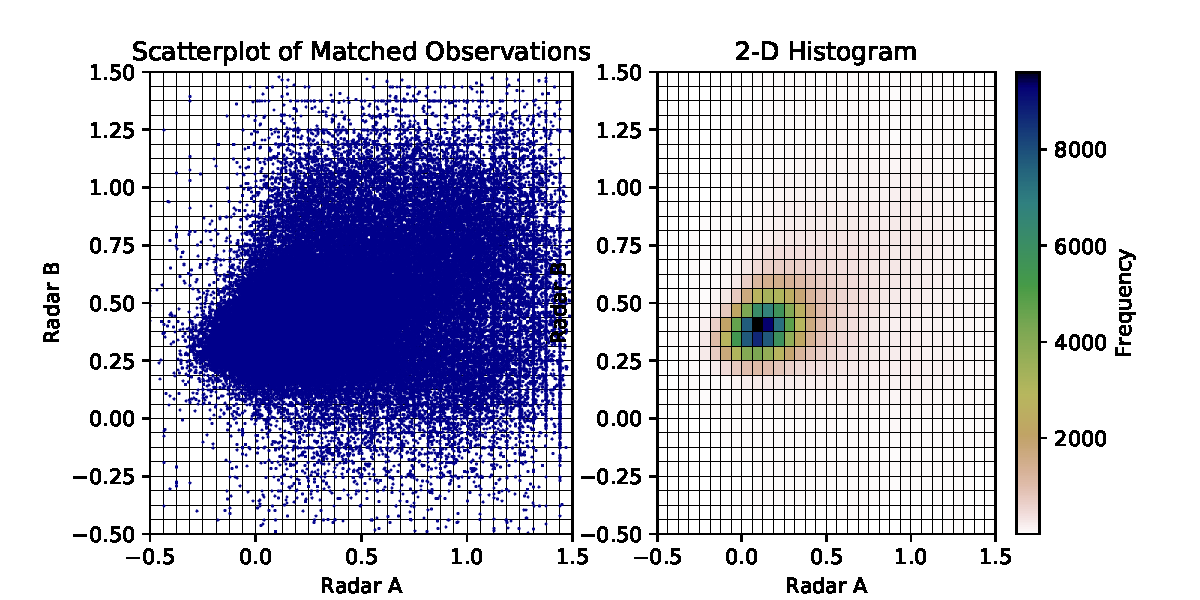
\includegraphics[width=\textwidth]{KDE_example}\centering
\caption{Scatter-plot of matched points illustrating the high density of the points (left). The total of points in this figure are 147,457. 2-D histogram of
the same matched points, binned to native data resolution (right).} 
\label{fig:KDE_example}
\end{figure}

\subsection{Orthonormal Linear Regression}
A hallmark of this study is the lack of ground truth. The sample sets compared contain error prone, independent variables. Typically, scatter-plots compare
an independent variable to a dependent variable. Instead of performing a standard linear regression between the variables, an orthonormal linear regression
is used. This type of regression allows for error in both variables, by performing the least squares regression perpendicular to the initial fit instead of
vertically \citep{Markovsky2007}. Figure \ref{fig:total_least_squares} demonstrates this concept.
\begin{figure}[H]
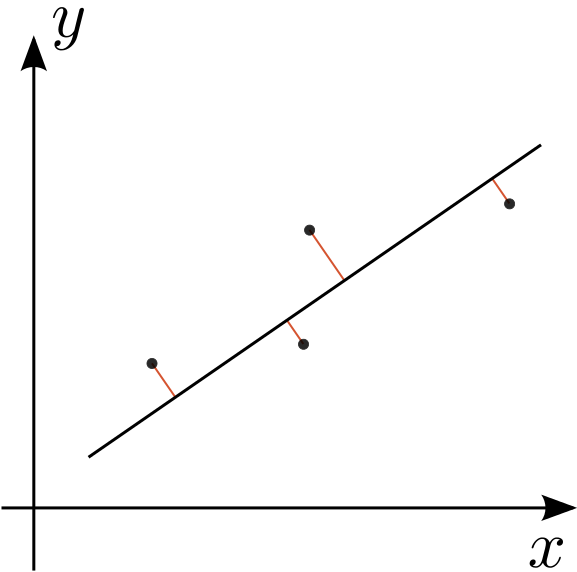
\includegraphics[scale=0.4]{total_least_square}\centering
\caption{Demonstration of an Orthonormal Linear Regression} 
\label{fig:total_least_squares}
\end{figure}
\section{$Z_{DR}$ Bias Estimation}
Although it not possible to check absolute calibration of $Z_{H}$ when comparing two radars, it is possible to verfiy $Z_{DR}$ calibration due to relative
nature of the quantity \citep{Zrnic2006}. While radars are regularly calibrated using internal calibration procedures, an external check is useful for
monitoring the time-varying component of calibration. The typical process for calibration of $Z_{DR}$ is pointing the antenna to zenith and performing ``bird
bath'' scans during light rain events \citep{Hubbert2006}. The $Z_{DR}$ in light rain is expected to be 0 dB, therefore any offset from this is considered a
bias; The signal processor subtracts out this bias to achieve the final output. Due to mechanical constraints, NEXRAD radars are unable to perform this
procedure, but CWKR is. NEXRAD radars disseminate a product which contains an estimate of $Z_{DR}$ bias using the intrinsic properties of
dry snow \cite{Zittel2015}. The daily published offset will be used to adjust $Z_{DR}$ values obtained from KBUF to diagnose any bias at CWKR. Under normal conditions, $Z_{DR}$ can be calibrated within 0.1 dB \citep{Zrnic2006}. This error threshold is adopted in this study.


\chapter{Chapter Three}

\section{Event Comparisons}
Now, we consider each of the selected events individually, demonstrating that the events were
classified correctly, and breaking down the results from each case. Although it is nearly impossible to
extricate lake influence from synoptically classified events, synoptic-scale ascent is considered the
characterizing factor. Descriptions of the synoptic pattern during each event are given without
reference; For reference, see Appendix A for the 500mb Geopotential Heights, Skew-T charts, and
Sounding Climatology utilized. These descriptions are ancillary to the study and are provided to
demonstrate a variety of patterns are represented.

\subsection{18 January 2014 - Synoptic}
In this event, a weak shortwave is approaching Southern Ontario as it rounds the base of a longwave
trough centered over the Eastern US. With the study area in the attendant
region of upper-level divergence, and a moist column present through 500mb, 
scattered snow showers form ahead of the shortwave. Figure \ref{fig:grid_ref_20140118} depicts
similiar cellular patterns between radars in the time-averaged $Z_{eH}$ field. In contrast, the $Z_{DR}$
comparison in Figure \ref{fig:grid_zdr_20140118}
shows that although the fields are similiar in their anisotropy, the spatial matching between the two is
tenuous everywhere but in the heaviest showers.

\begin{figure}[H]
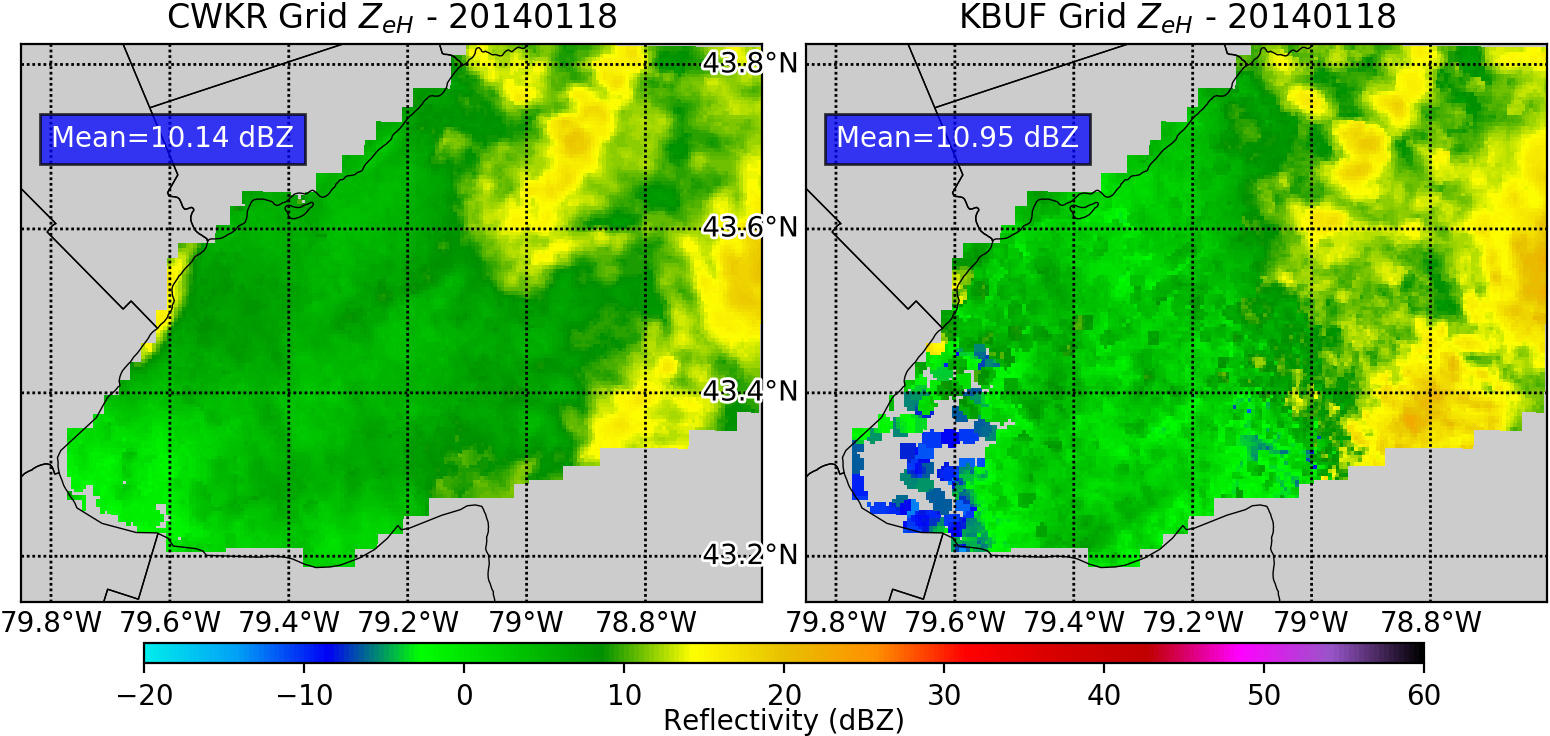
\includegraphics[width=\textwidth]{grid/ref/20140118}
\caption{Gridded $Z_{eH}$ comparison for 18 January 2014. Time-average of all admitted scans.} 
\label{fig:grid_ref_20140118}
\end{figure}

\begin{figure}[H]
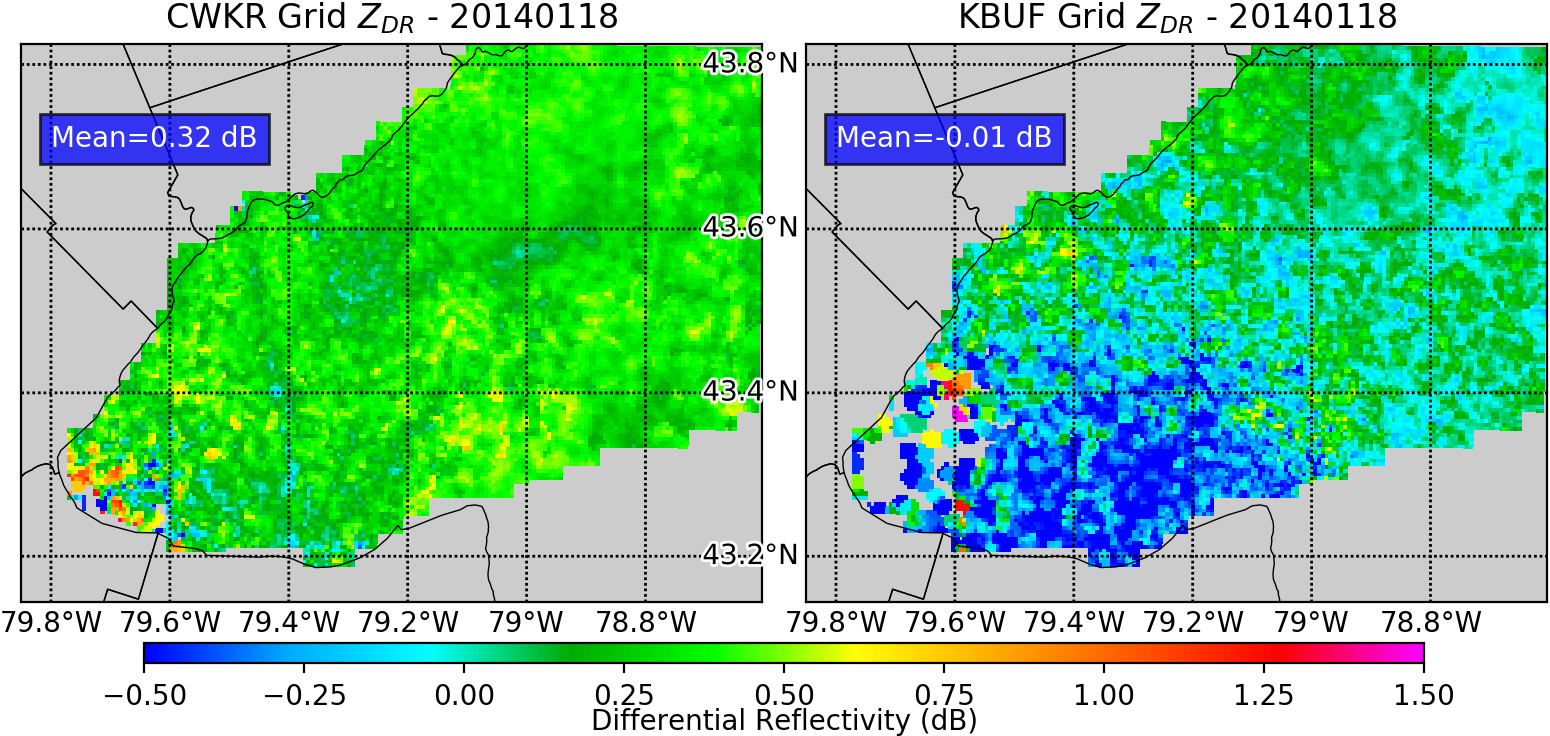
\includegraphics[width=\textwidth]{grid/zdr/20140118}
\caption{Gridded $Z_{DR}$ comparison for 18 January 2014. Time-average of all admitted scans.} 
\label{fig:grid_zdr_20140118}
\end{figure}
\vspace{5mm}

To investigate further, we examine a scatter-plot directly comparing matched values between radars.
Artifacts are present in both moments in Figure
\ref{fig:scatter_20140118}, indicated by evenly spaced vertical lines; these indicate an anomaly
originating from the axis of which they are normal to. For
$Z_{eH}$, Figure \ref{fig:scatter_ref_20140118} shows that artifacts are no longer present for values
greater than 15 dBZ, which indicates that a
stronger weather signal leads to better matching. On the contrary, Figure \ref{fig:scatter_zdr_20140118}
shows that for $Z_{DR}$, artifacts are present throughout. Also, the distribution of $Z_{DR}$ is unimodal. 

\begin{figure}[H]
\centering
   \begin{subfigure}{0.49\linewidth} \centering
     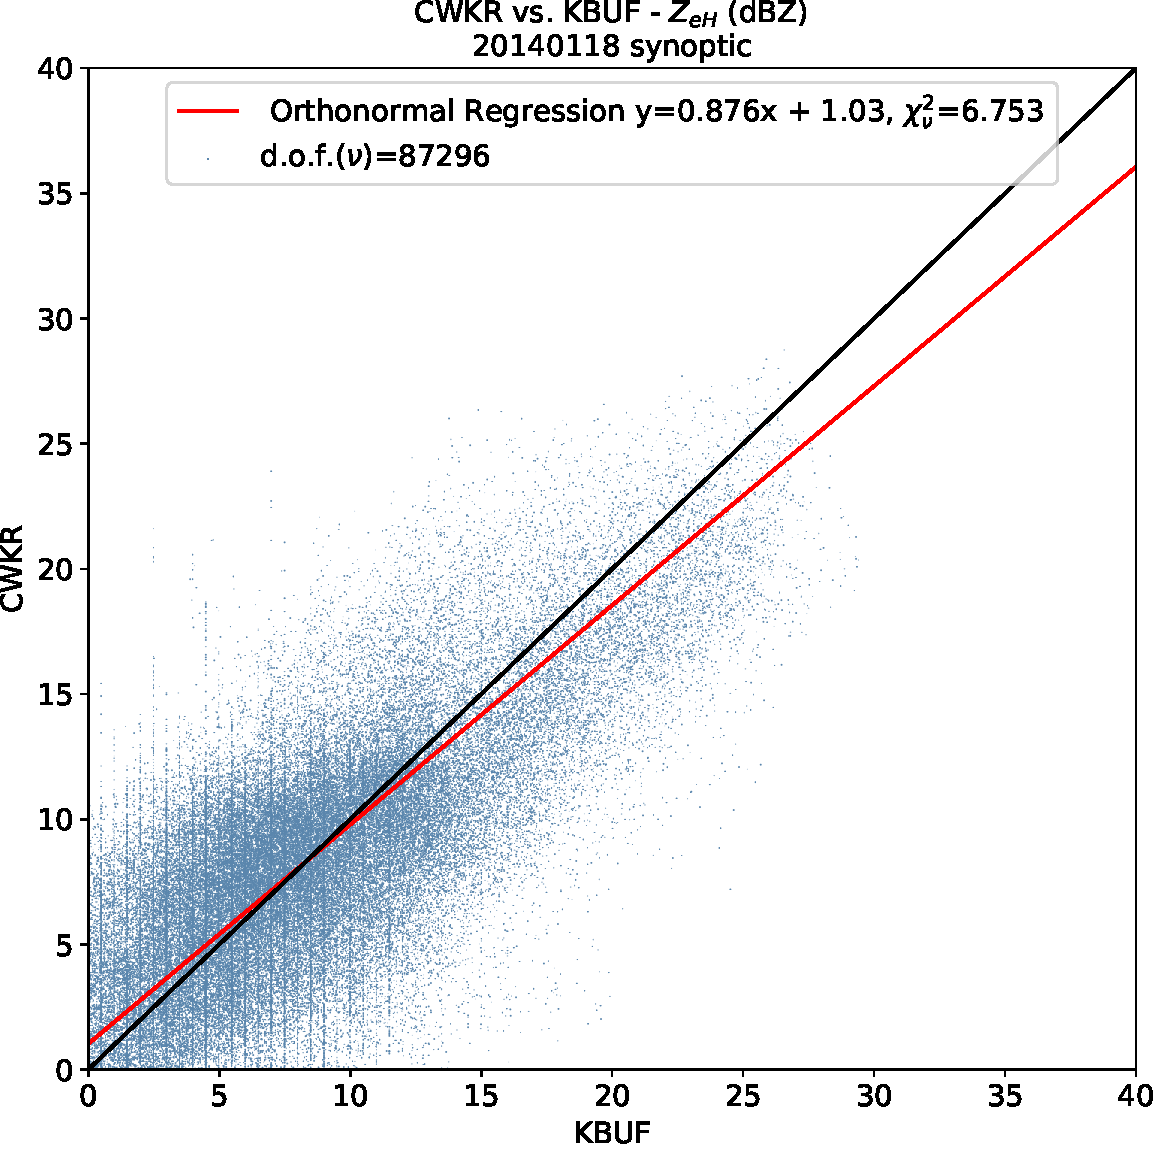
\includegraphics[scale=0.38]{scatter/ref/20140118}
     \caption{$Z_{eH}$ (dBZ)}\label{fig:scatter_ref_20140118}
   \end{subfigure}
   \begin{subfigure}{0.49\linewidth} \centering
     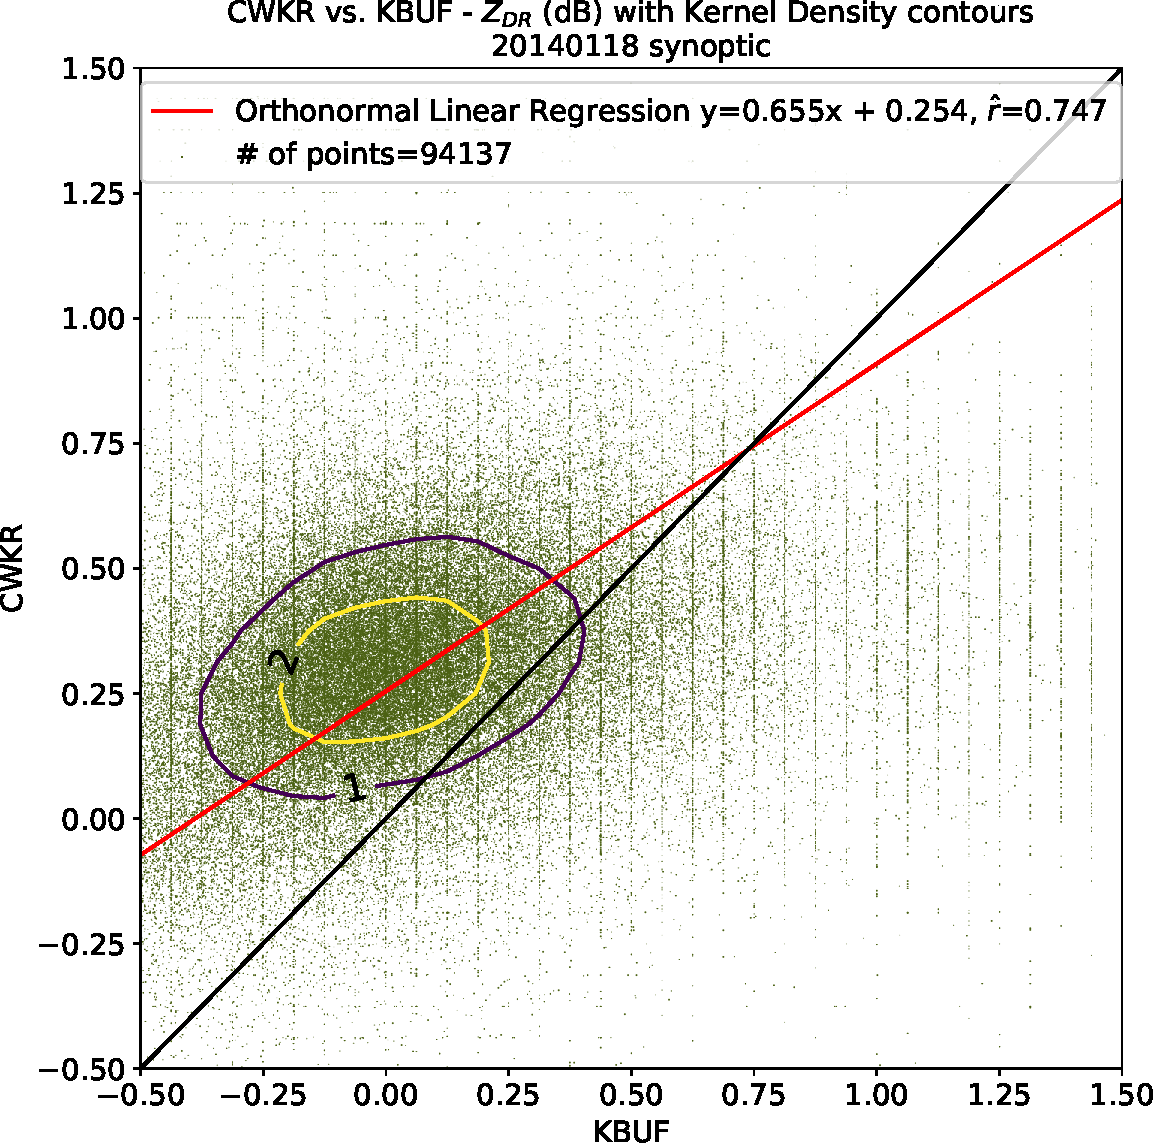
\includegraphics[scale=0.38]{scatter/zdr/20140118}
     \caption{$Z_{DR}$ (dB)}\label{fig:scatter_zdr_20140118}
   \end{subfigure}
\caption{Direct comparisons for 18 January 2014. Dataset includes all admitted grid cells.} \label{fig:scatter_20140118}
\end{figure}

It is still possible to extract a signal from the noise though, by only including data points with a
normalized kernel density estimate greater than or equal to two. These points are used to resolve the bias present in
$Z_{DR}$, as suggested by the comparisons. Figure \ref{fig:hist_20140118} gives an estimate of the
bias at CWKR by using this method and the known bias at KBUF as provided by the NEXRAD
External Target Bias Estimation technique. This method yields a median of -0.095 dB for the bias at CWKR, which when
considered with the error threshold of $\pm$0.1 dB, indicates no discernible bias.

\begin{figure}[H]
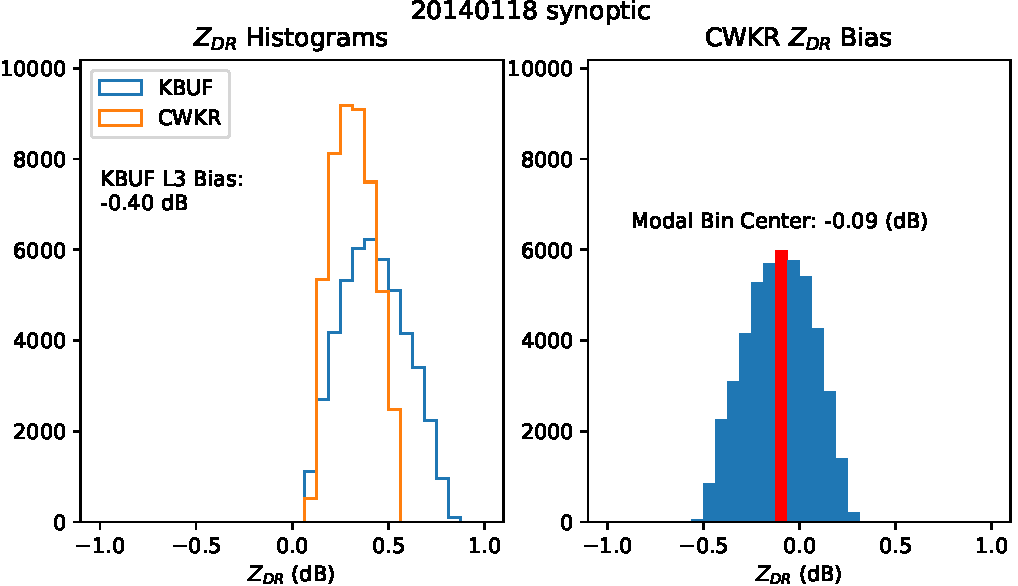
\includegraphics[width=0.75\textwidth]{hist/20140118}\centering
\caption{Histograms of $Z_{DR}$ (left), $Z_{DR}$ bias at CWKR, determined by subtracting the gridded, bias adjusted $Z_{DR}$ at KBUF from the $Z_{DR}$ at
CWKR. Both datasets include only matched points with KDE $\geq 2$. } 
\label{fig:hist_20140118}
\end{figure}



\begin{figure}[p]
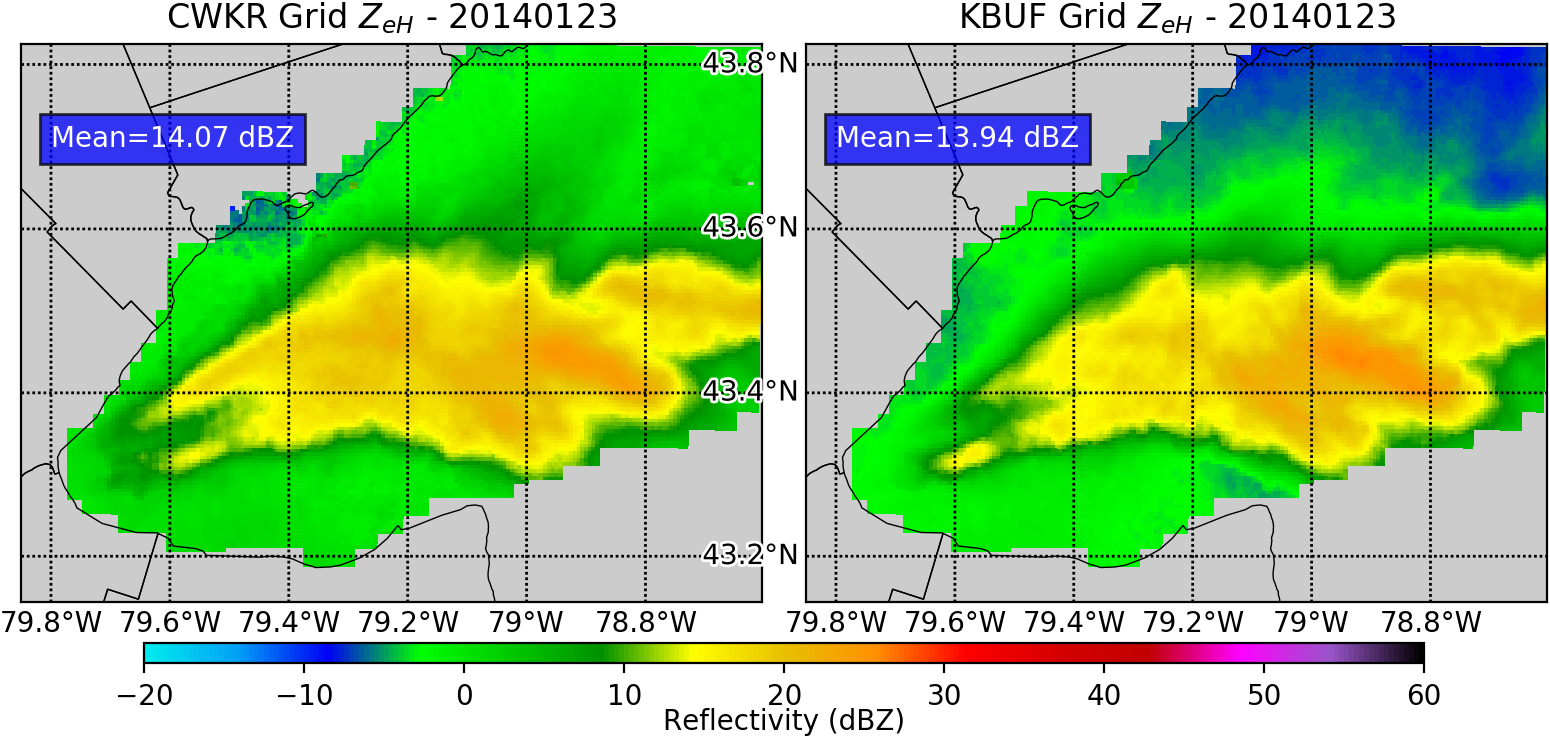
\includegraphics[width=\textwidth]{grid/ref/20140123}
\caption{Gridded $Z_{eH}$ comparison for 23 January 2014. Time-average of all admitted scans.} 
\label{fig:grid_ref_20140123}
\end{figure}

\begin{figure}[p]
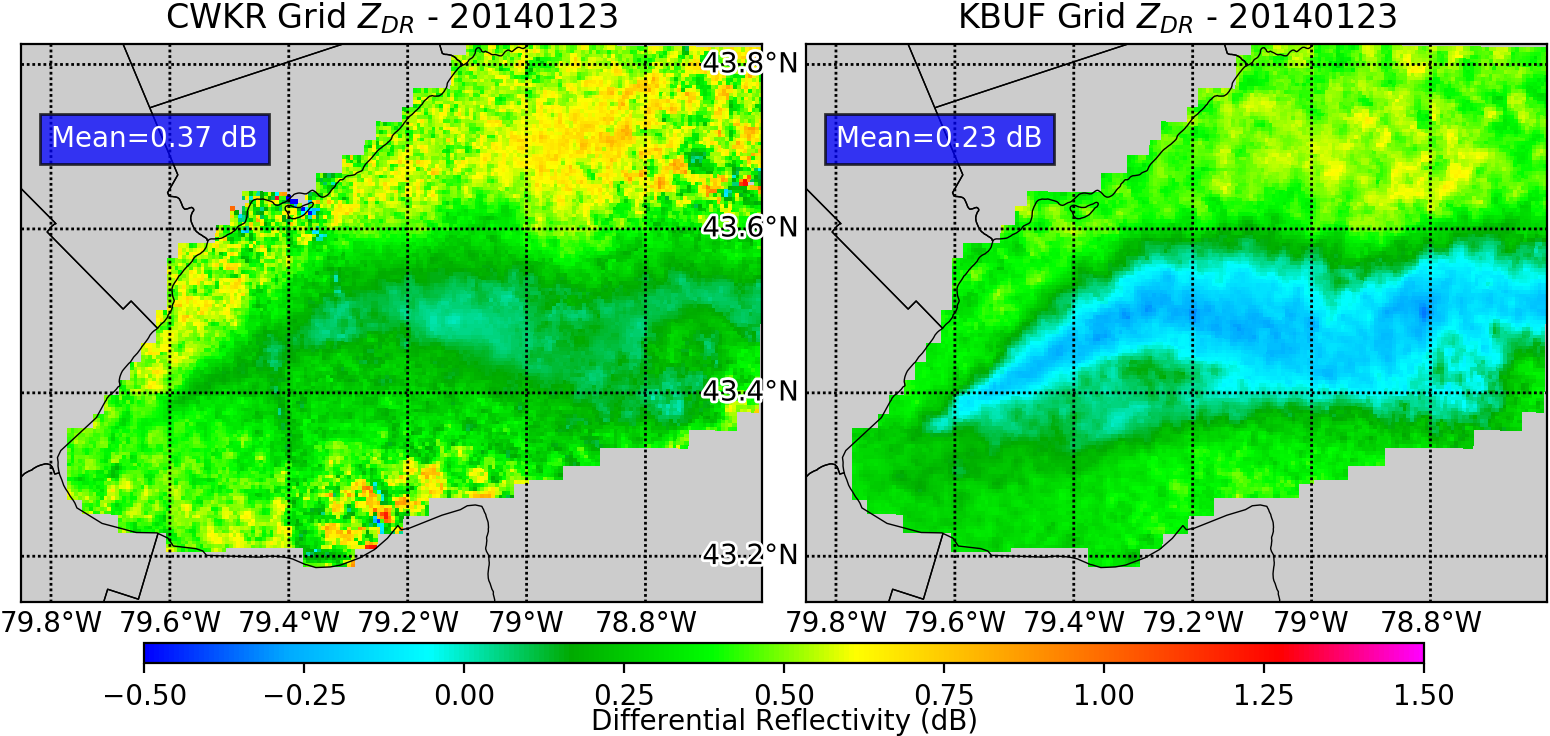
\includegraphics[width=\textwidth]{grid/zdr/20140123}
\caption{Gridded $Z_{DR}$ comparison for 23 January 2014. Time-average of all admitted scans.} 
\label{fig:grid_zdr_20140123}
\end{figure}

\subsection{23 January 2014 - Lake-Effect}
A positively tilted longwave trough dominates the eastern third of Canada during this event, with NW
winds at 850mb and SW winds at the surface. This light yet convergent flow yields the single, heavy
band depicted in Figure \ref{fig:grid_ref_20140123}, colloquially referred to as ``tea-kettle'' lake-effect
snow. There is also a background stream of very light lake-effect snow impinging from Lake Erie.
Spatial banding patterns of the lake-effect snow in the time-averaged $Z_{eH}$ fields as compared 
between the radars are remarkably similar. The difference between the grid mean values are within only
0.13 dBZ. In contrast, the $Z_{DR}$ comparison indicates that
although the fields are similiar in their anisotropy, the spatial matching between the two is tenuous
everywhere but in the heaviest showers. An anistropic pattern is also imparted on the $Z_{DR}$ fields
by the light snow from Lake Erie, evident in Figure \ref{fig:grid_zdr_20140123}. The scatter-plot in Figure \ref{fig:scatter_ref_20140123} shows an analysis
free of artifacts, and good agreement on average between radars. Although the agreement in $Z_{eH}$ between radars as
indicated by the orthonormal regression is acceptable, the chi-square
statistic indicates a high error variance. A slightly bi-modal distribution of $Z_{DR}$ is shown in 
Figure \ref{fig:scatter_ref_20140123}, with the main peak near 0 dB and a secondary peak near 0.5 dB, with artifacts much more prevalent near the secondary
peak. Both analysis methods have indicated a bias in $Z_{DR}$, so the
kernel density method for estimating bias is used. Figure \ref{fig:hist_20140123} shows an estimate of
the bias at CWKR, with a median value of -0.055 dB. Once again, no discernible bias exists outside of the error
threshold of $\pm$0.1 dB for this event.

\begin{figure}[H]
\centering
   \begin{subfigure}{0.49\linewidth} \centering
     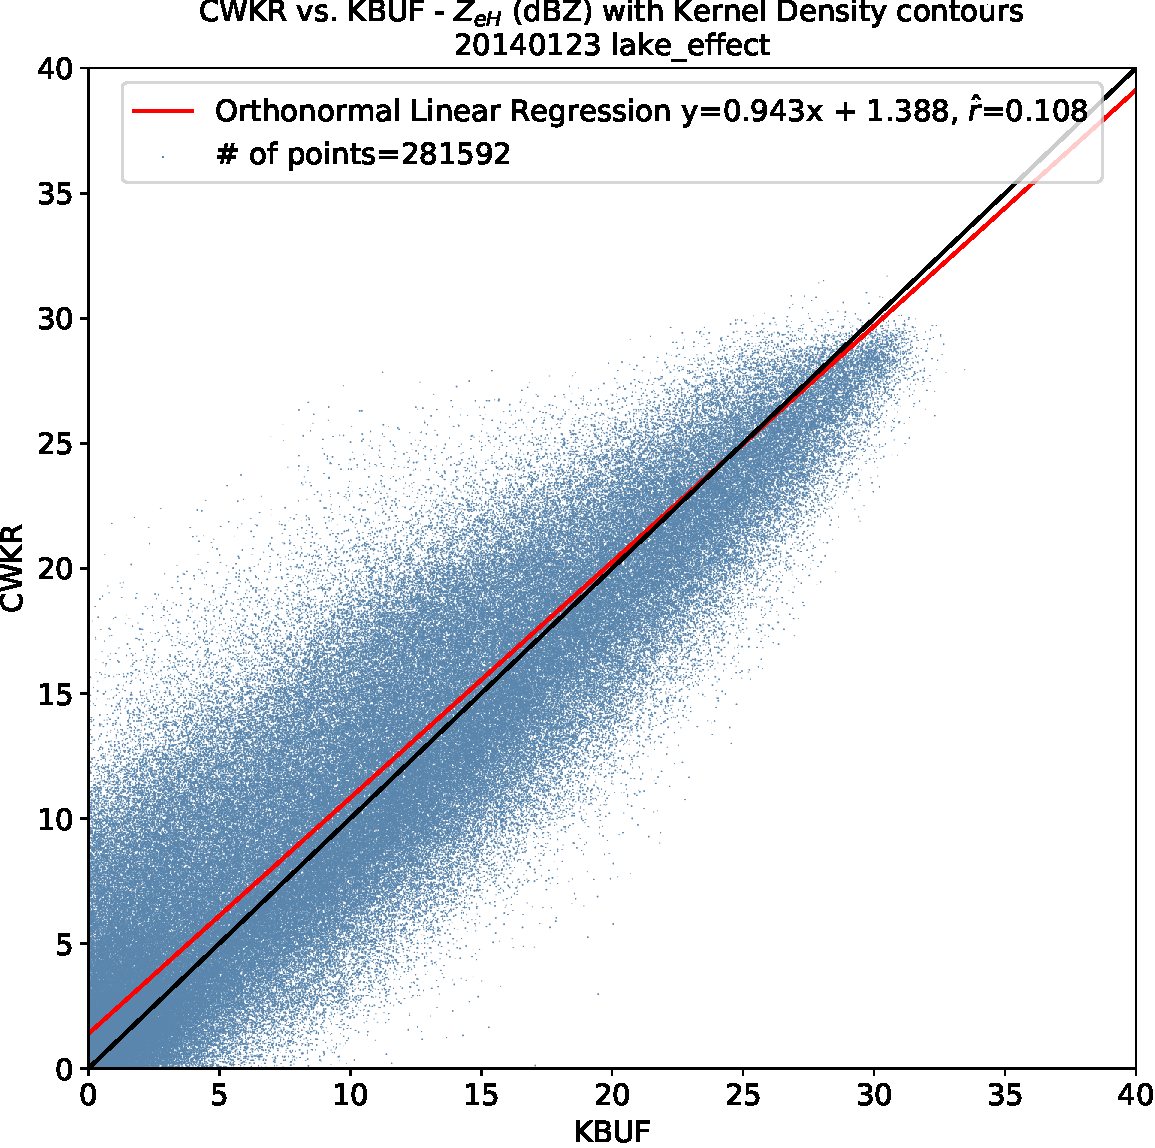
\includegraphics[scale=0.38]{scatter/ref/20140123}
     \caption{$Z_{eH}$ (dBZ)}\label{fig:scatter_ref_20140123}
   \end{subfigure}
   \begin{subfigure}{0.49\linewidth} \centering
     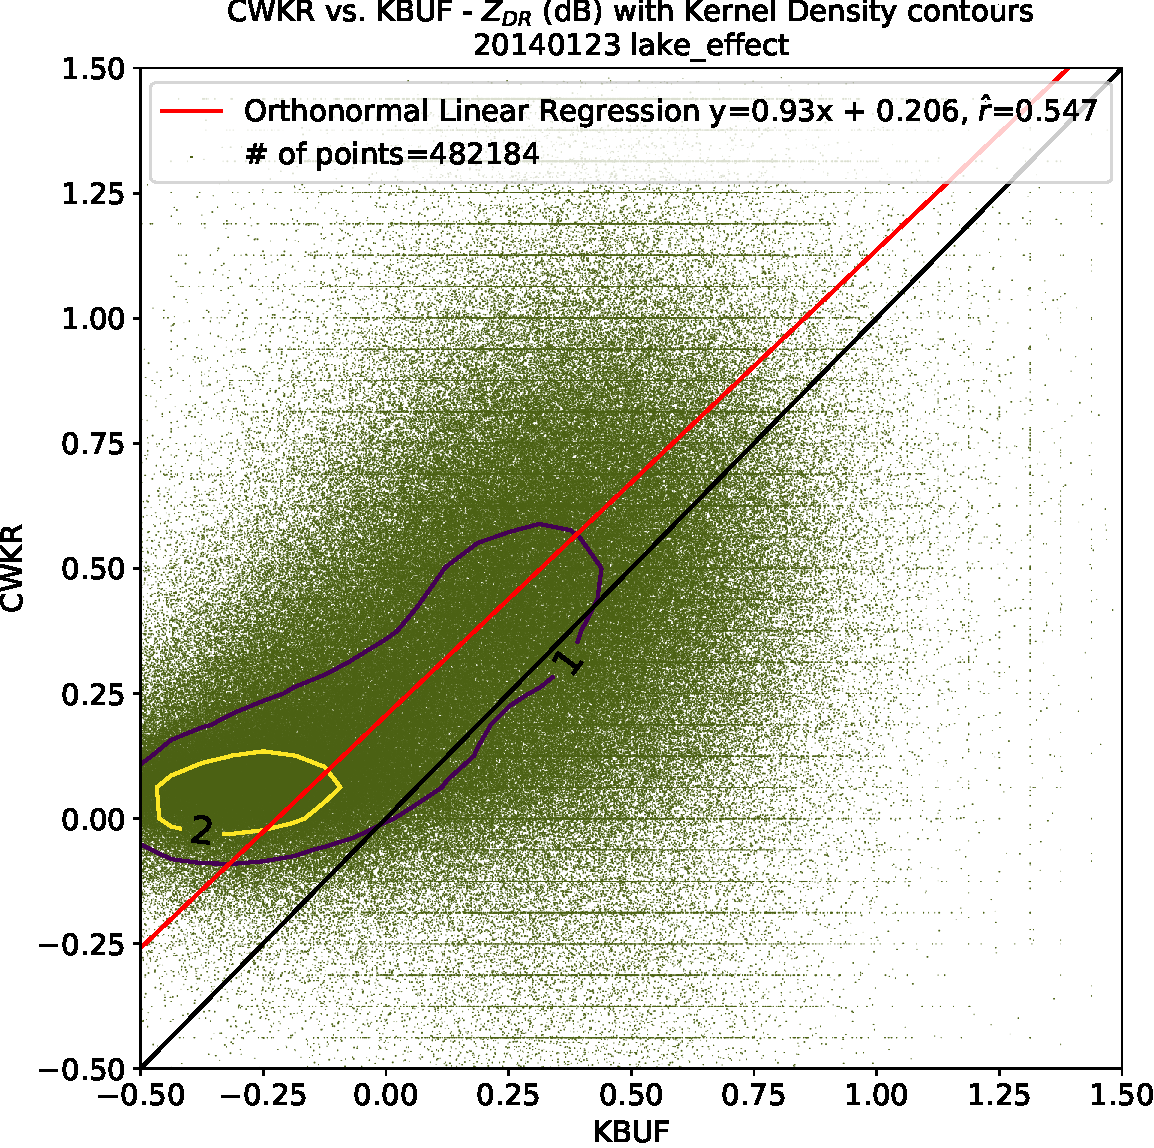
\includegraphics[scale=0.38]{scatter/zdr/20140123}
     \caption{$Z_{DR}$ (dB)}\label{fig:scatter_zdr_20140123}
   \end{subfigure}
\caption{Direct comparisons for 23 January 2014. Dataset includes all admitted grid cells.}
\label{fig:scatter_20140123}
\end{figure}

\begin{figure}[H]
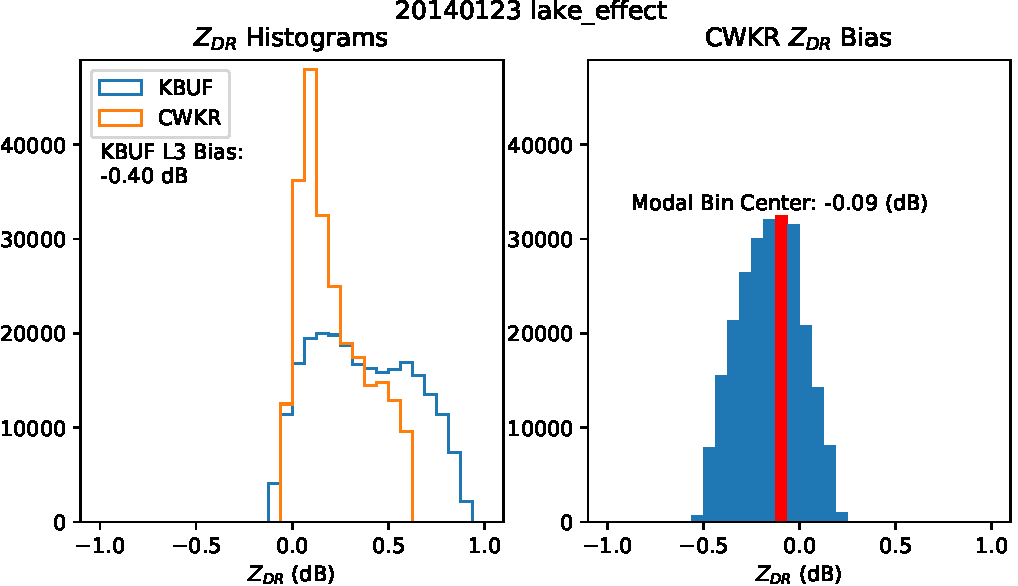
\includegraphics[width=0.75\textwidth]{hist/20140123}\centering
\caption{Histograms of $Z_{DR}$ (left), $Z_{DR}$ bias at CWKR, determined by subtracting the
gridded, bias adjusted $Z_{DR}$ at KBUF from the $Z_{DR}$ at CWKR. Both datasets include only
matched points with KDE $\geq 2$. } 
\label{fig:hist_20140123}
\end{figure}

\subsection{1 February 2014 - Synoptic}
This event is characterized by strong SW flow aloft, with above average moisture content. This leads to
widespread stratiform snow, with an eventual transition to rain outside of the time interval selected.
A large swath of steady snow is depicted by the time-averaged $Z_{eH}$ in Figure \ref{fig:grid_ref_20140201}. 
Furthermore, Figure \ref{fig:grid_zdr_20140201} shows smoother $Z_{DR}$
fields as compared with other events, which confirms the stratiform nature of the precipitation. Next, Figure \ref{fig:scatter_ref_20140201} indicates very
good agreement in $Z_{eH}$ with low error variance, while Figure \ref{fig:scatter_zdr_20140201} shows a very dense uni-modal, biased kernel for $Z_{DR}$. The
histogram in Figure \ref{fig:hist_20140201} reveals that the anomalous bias between the radars is indicative of a $Z_{DR}$ bias at CWKR, with a value of
0.217 dB. The source of this bias will be discussed in the next chapter.

\begin{figure}[H]
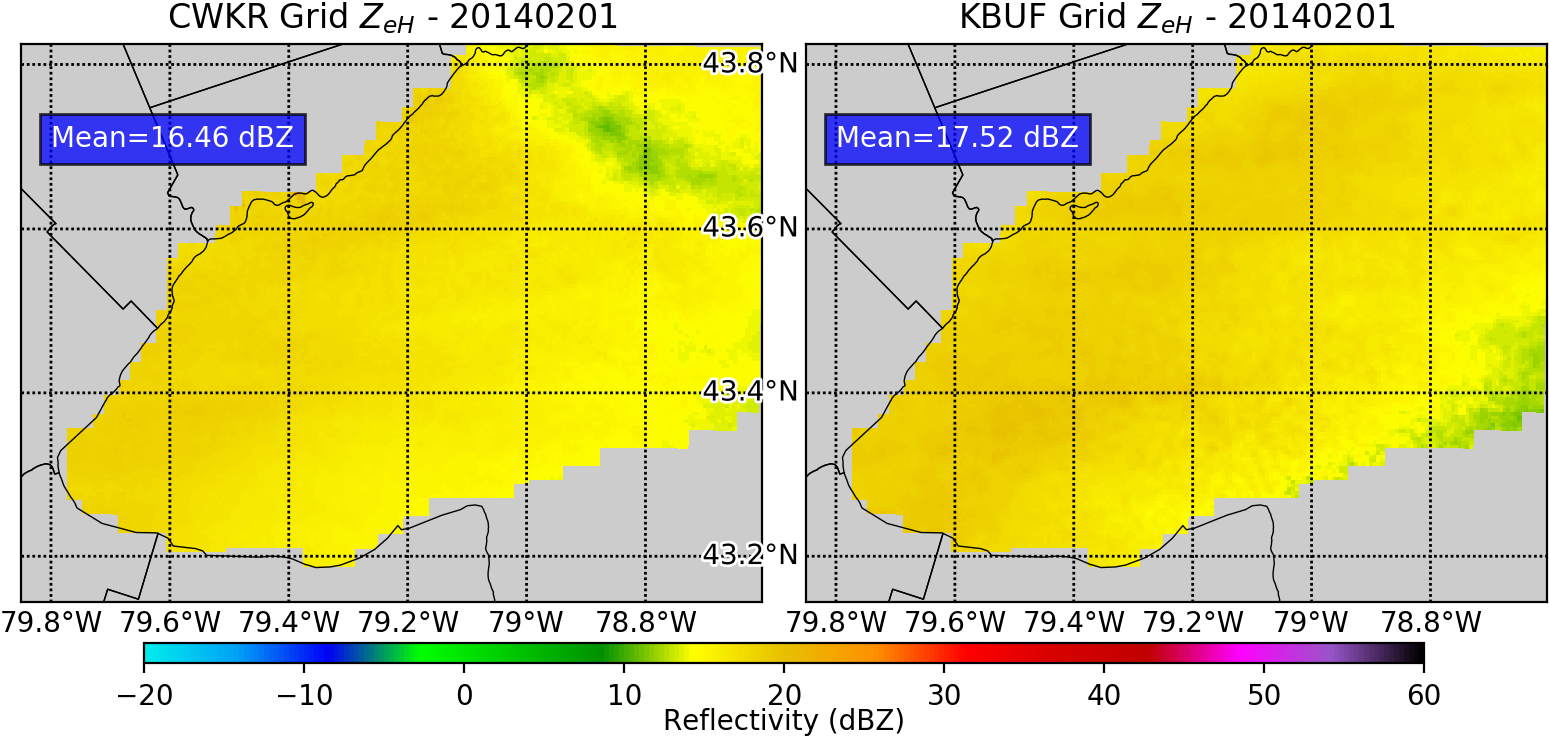
\includegraphics[width=\textwidth]{grid/ref/20140201}
\caption{Gridded $Z_{eH}$ comparison for 1 February 2014. Time-average of all admitted scans.} 
\label{fig:grid_ref_20140201}
\end{figure}

\begin{figure}[H]
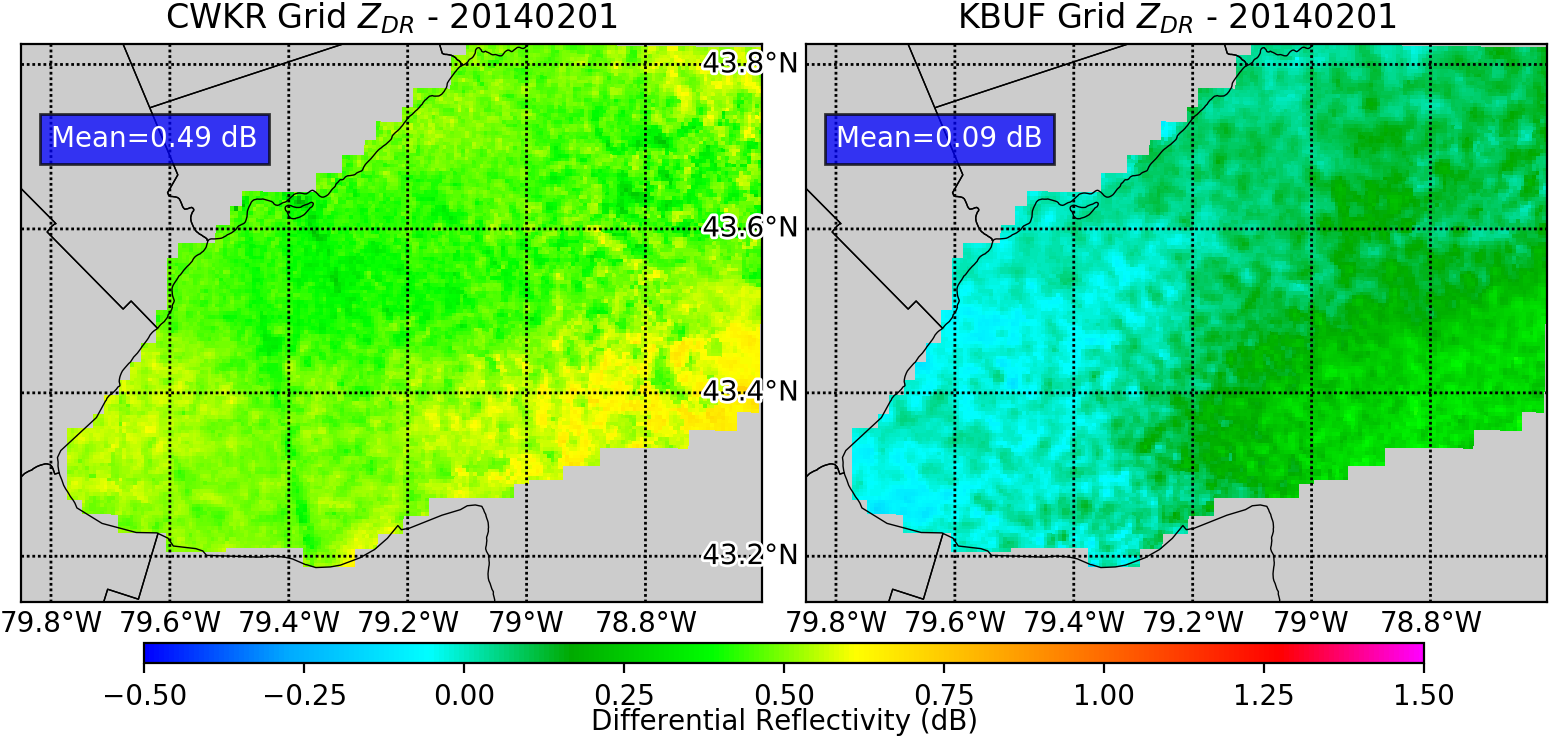
\includegraphics[width=\textwidth]{grid/zdr/20140201}
\caption{Gridded $Z_{DR}$ comparison for 1 February 2014. Time-average of all admitted scans.} 
\label{fig:grid_zdr_20140201}
\end{figure}

\begin{figure}[H]
\centering
   \begin{subfigure}{0.49\linewidth} \centering
     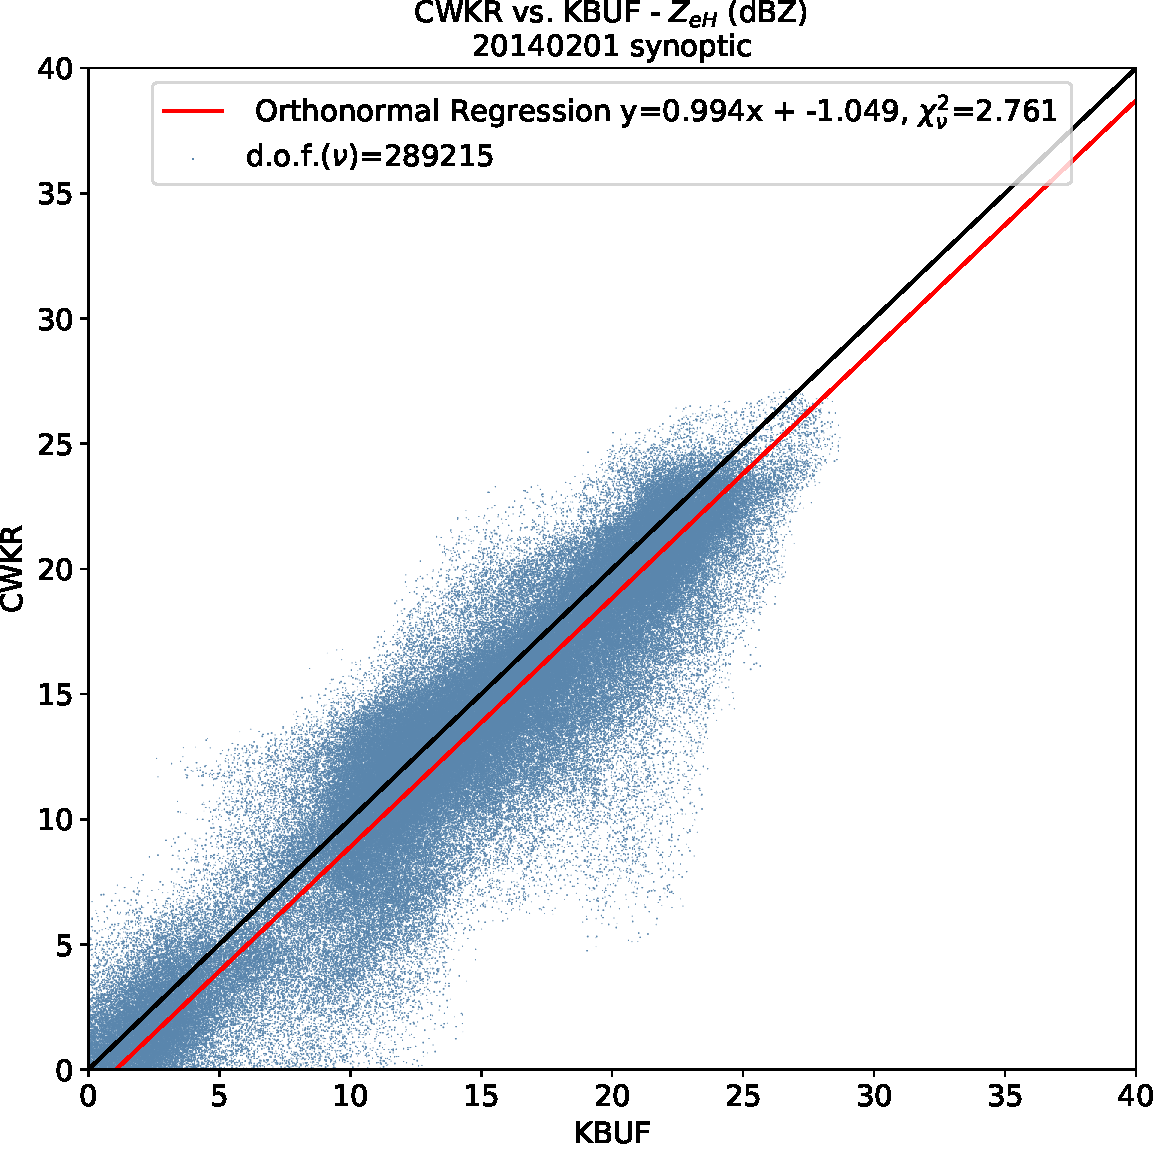
\includegraphics[scale=0.38]{scatter/ref/20140201}
     \caption{$Z_{eH}$ (dBZ)}\label{fig:scatter_ref_20140201}
   \end{subfigure}
   \begin{subfigure}{0.49\linewidth} \centering
     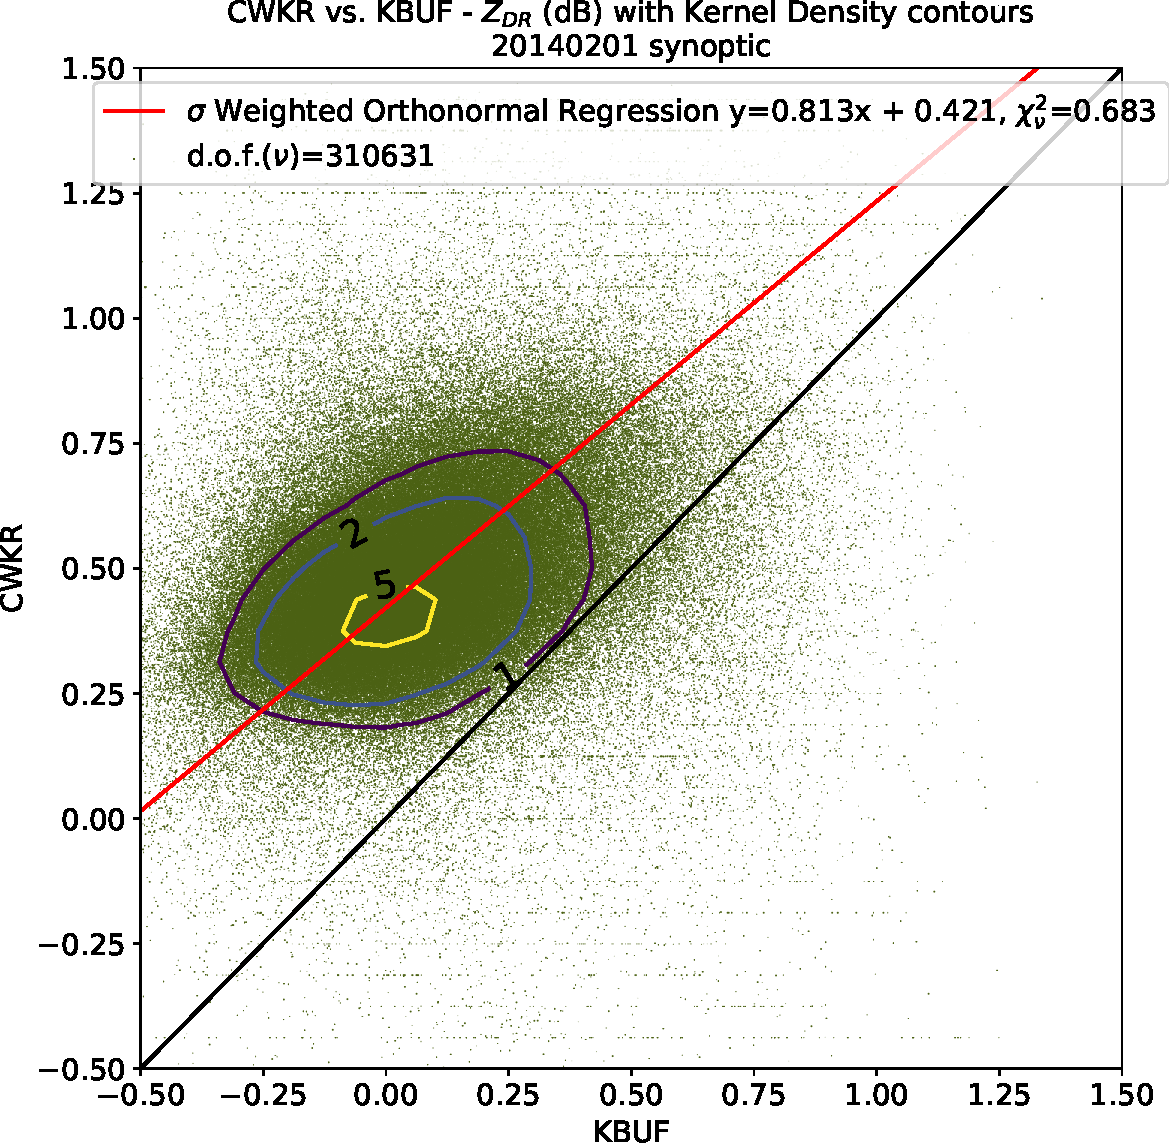
\includegraphics[scale=0.38]{scatter/zdr/20140201}
     \caption{$Z_{DR}$ (dB)}\label{fig:scatter_zdr_20140201}
   \end{subfigure}
\caption{Direct comparisons for 1 February 2014. Dataset includes all admitted grid cells.} \label{fig:scatter_20140201}
\end{figure}

\begin{figure}[H]
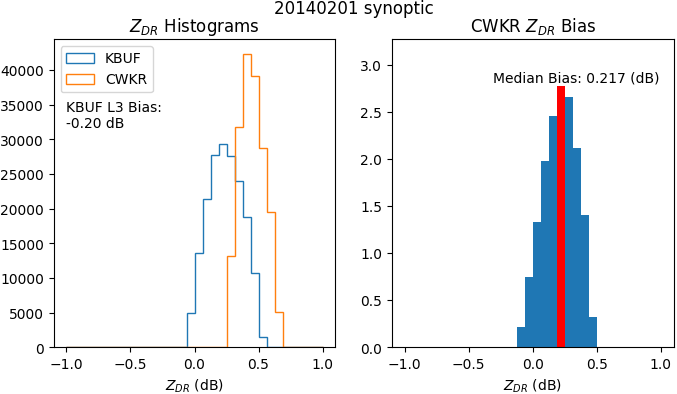
\includegraphics[width=0.75\textwidth]{hist/20140201}\centering
\caption{Histograms of $Z_{DR}$ (left), $Z_{DR}$ bias at CWKR, determined by subtracting the gridded, bias adjusted $Z_{DR}$ at KBUF from the $Z_{DR}$ at
CWKR. Both datasets include only matched points with KDE $\geq 2$. } 
\label{fig:hist_20140201}
\end{figure}

\subsection{6 January 2015 - Lake-Effect}
A highly zonal, NW flow aloft is present in this case, a typical pattern for lake-effect snow across the Great Lakes region. Anemic in radar appearance, a
lake-effect band develops in the light winds near the surface; this case could be characterized as a weak ``tea-kettle'' event. Figure
\ref{fig:grid_ref_20150106} depicts stationary banding in the time-averaged $Z_{eH}$. Of note is that CWKR observes more of the finer scale features as
compared with KBUF, also evidenced by the +2.9 dBZ difference in $Z_{eH}$ mean. 
\begin{figure}[H]
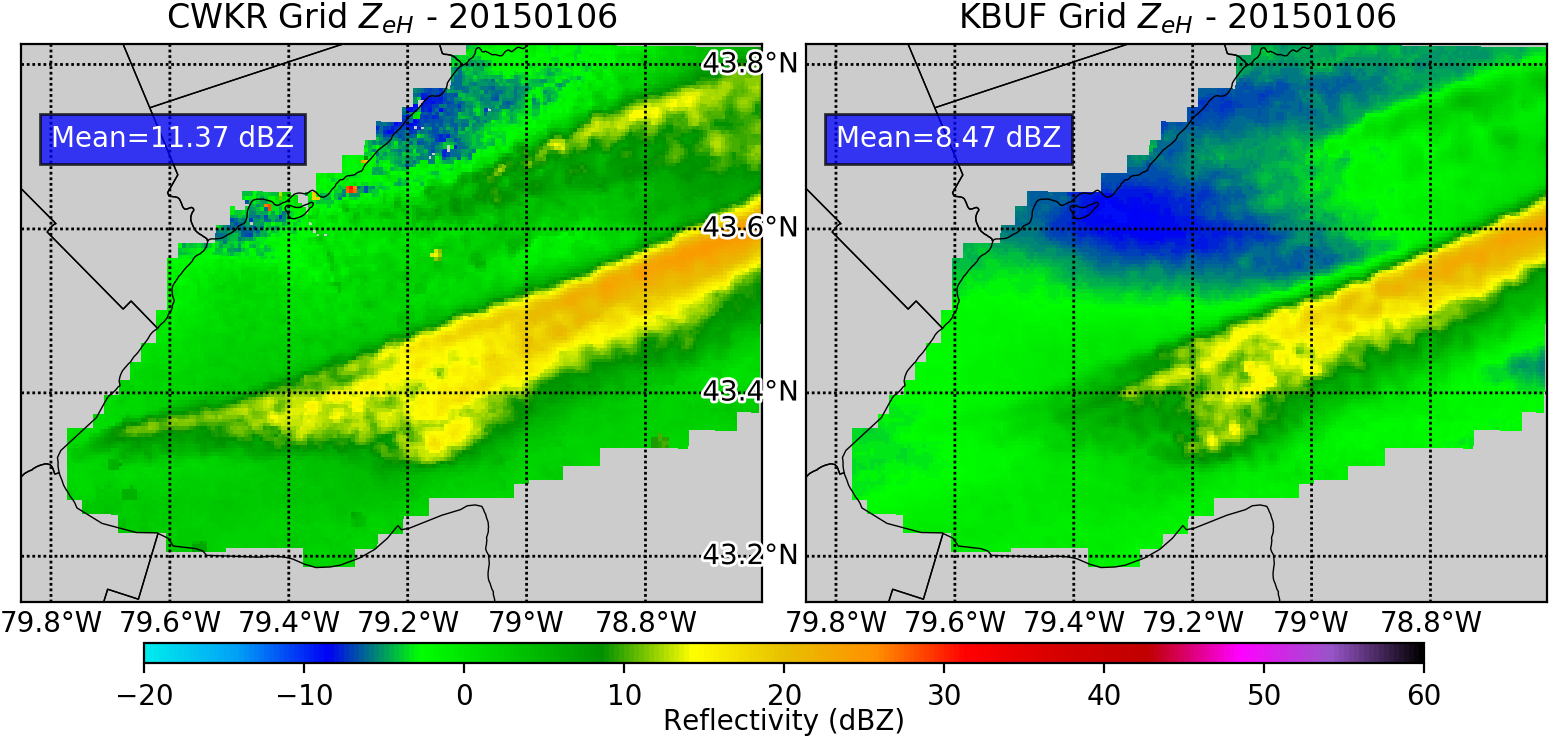
\includegraphics[width=\textwidth]{grid/ref/20150106}
\caption{Gridded $Z_{eH}$ comparison for 6 January 2015. Time-average of all admitted scans.} 
\label{fig:grid_ref_20150106}
\end{figure}
This case stands out from the rest in terms of $Z_{DR}$, as the fields are
very similiar and unbiased as shown in Figure \ref{fig:grid_zdr_20150106}. The scatter-plot in Figure
\ref{fig:scatter_ref_20150106} confirms what is shown in the gridded $Z_{eH}$, with values skewed higher for CWKR. Figure \ref{fig:scatter_zdr_20150106}
shows a bi-modal distribution for $Z_{DR}$, with the
main peak around 0.5 dB and a secondary peak near 0 dB. The histogram in Figure
\ref{fig:hist_20150106} confirms the observed unbiased $Z_{DR}$, with a near zero median value of 0.003 dB.


\begin{figure}[H]
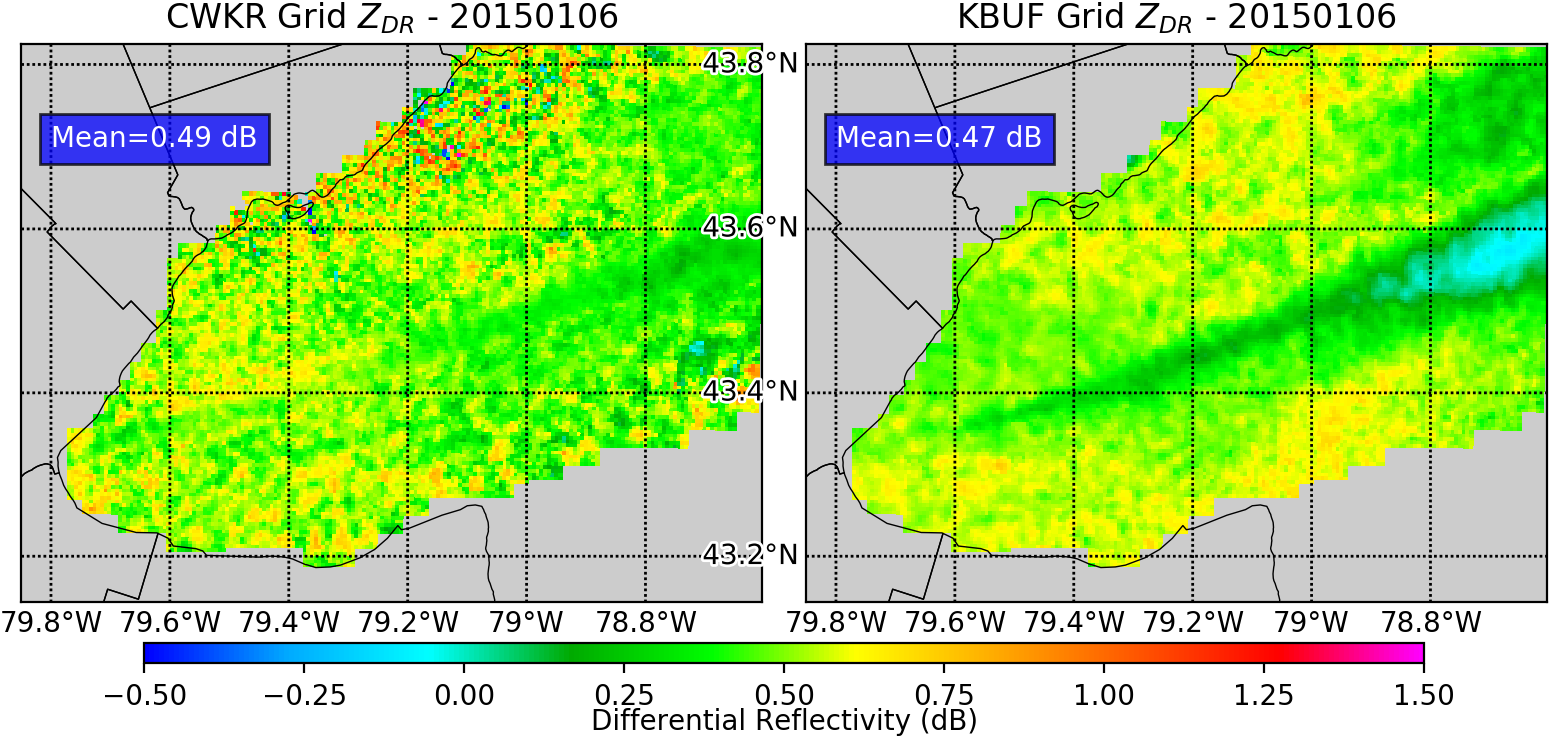
\includegraphics[width=\textwidth]{grid/zdr/20150106}
\caption{Gridded $Z_{DR}$ comparison for 6 January 2015. Time-average of all admitted scans.} 
\label{fig:grid_zdr_20150106}
\end{figure}

\begin{figure}[H]
\centering
   \begin{subfigure}{0.49\linewidth} \centering
     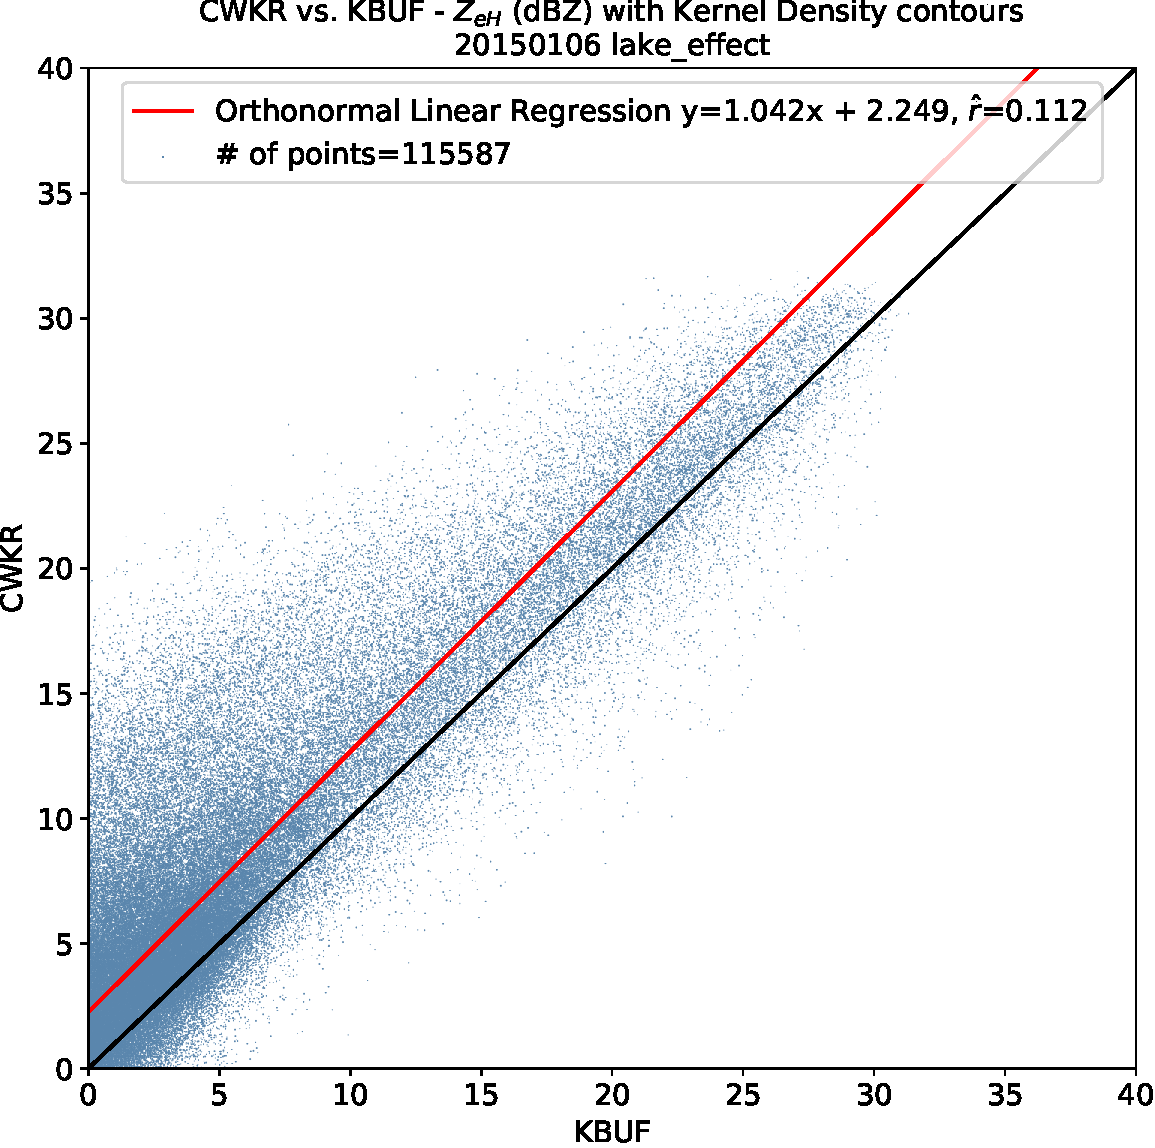
\includegraphics[scale=0.38]{scatter/ref/20150106}
     \caption{$Z_{eH}$ (dBZ)}\label{fig:scatter_ref_20150106}
   \end{subfigure}
   \begin{subfigure}{0.49\linewidth} \centering
     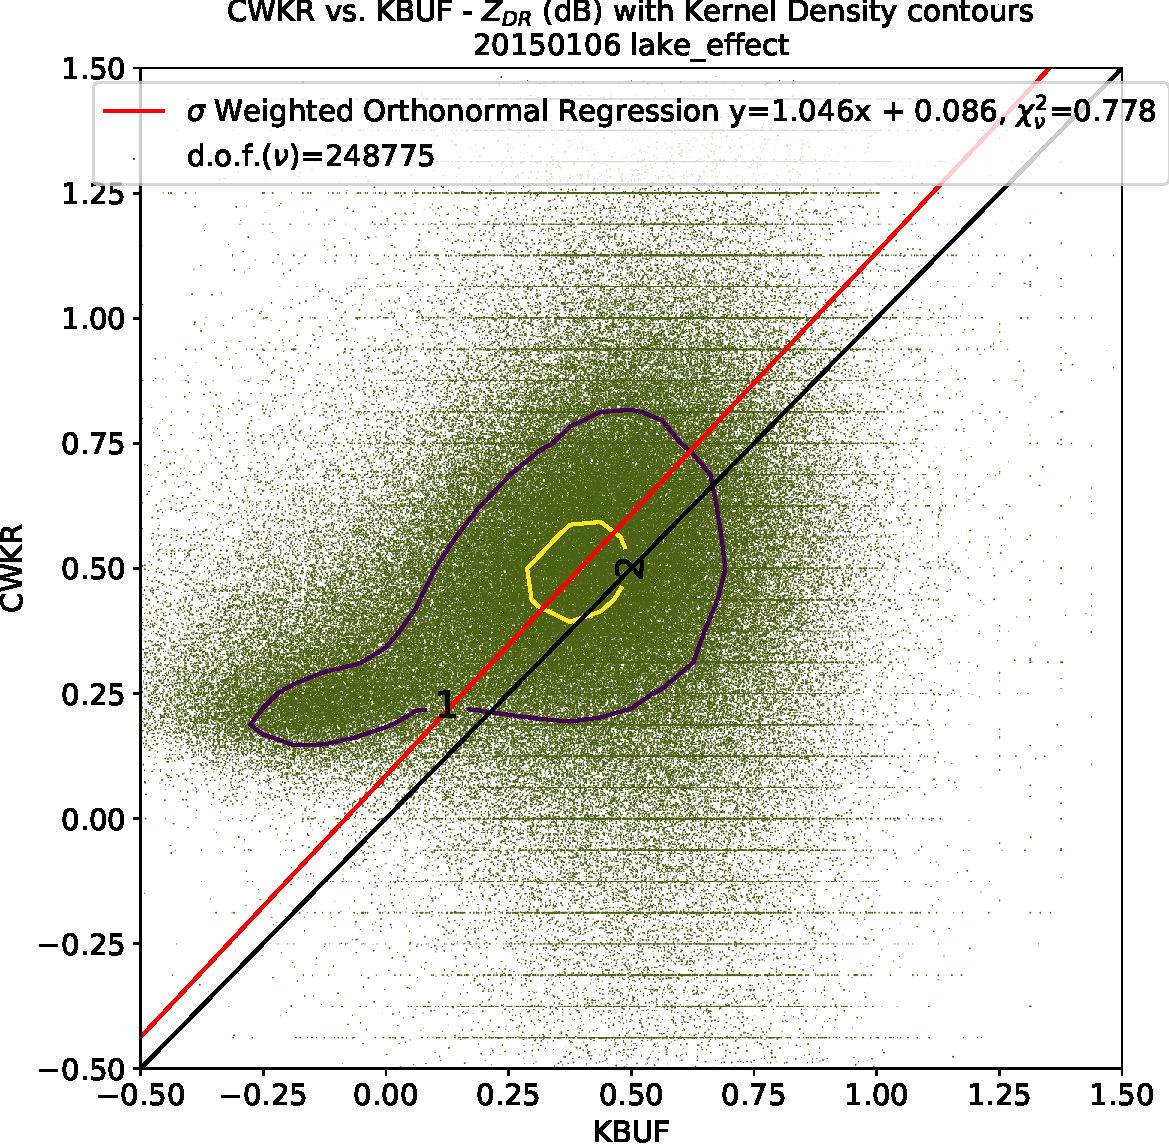
\includegraphics[scale=0.38]{scatter/zdr/20150106}
     \caption{$Z_{DR}$ (dB)}\label{fig:scatter_zdr_20150106}
   \end{subfigure}
\caption{Direct comparisons for 6 January 2015. Dataset includes all admitted grid cells.} \label{fig:scatter_20150106}
\end{figure}

\begin{figure}[H]
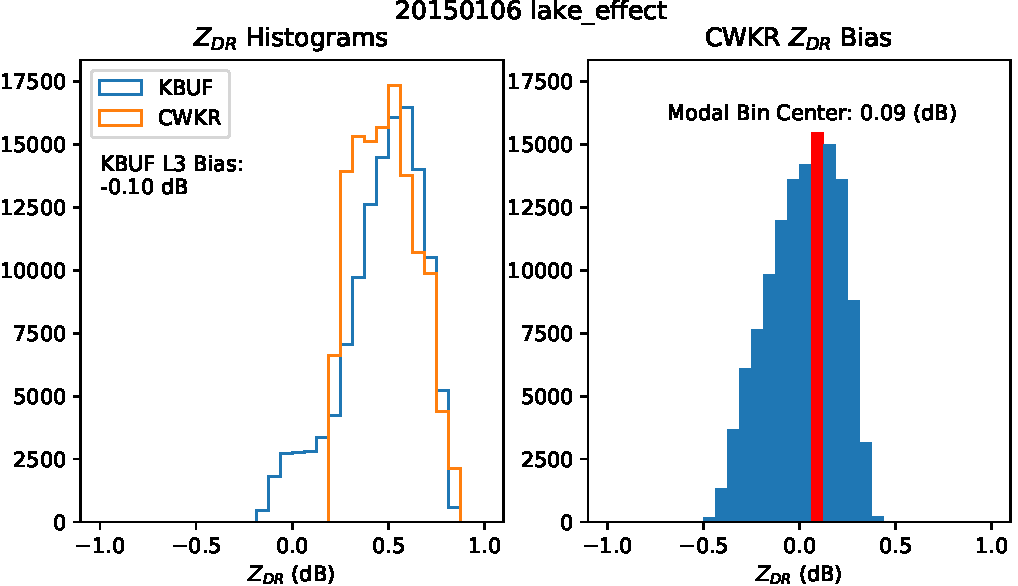
\includegraphics[width=0.75\textwidth]{hist/20150106}\centering
\caption{Histograms of $Z_{DR}$ (left), $Z_{DR}$ bias at CWKR, determined by subtracting the gridded, bias adjusted $Z_{DR}$ at KBUF from the $Z_{DR}$ at
CWKR. Both datasets include only matched points with KDE $\geq 2$. } 
\label{fig:hist_20150106}
\end{figure}

\subsection{7 January 2015 - Synoptic}
Less than 24 hours after the previous event, the zonal flow has buckled and a strong shortwave is overhead Southern Ontario. Radar animations indicate a
frontally forced band of snow showers. Figure \ref{fig:grid_ref_20150107} shows the solid band of snow progressed from mid-lake southward, with similiar
depictions of $Z_{eH}$ between radars. Inspection of the scatter-plot in Figure \ref{fig:scatter_ref_20150107} indicates good agreement with reasonable error
variance, while Figure \ref{fig:scatter_zdr_20150107} shows a uni-modal distribution of $Z_{DR}$ with a relatively dense kernel.
Meanwhile, Figure \ref{fig:grid_zdr_20150107} shows two anisotropic fields, especially noisy in areas of light returns. 
Estimating the bias at CWKR, the histogram in Figure \ref{fig:hist_20150107} gives a median value of -0.040 dB. This indicates that no discernible bias
exists outside of the error threshold of $\pm$0.1 dB for this event.

\begin{figure}[H]
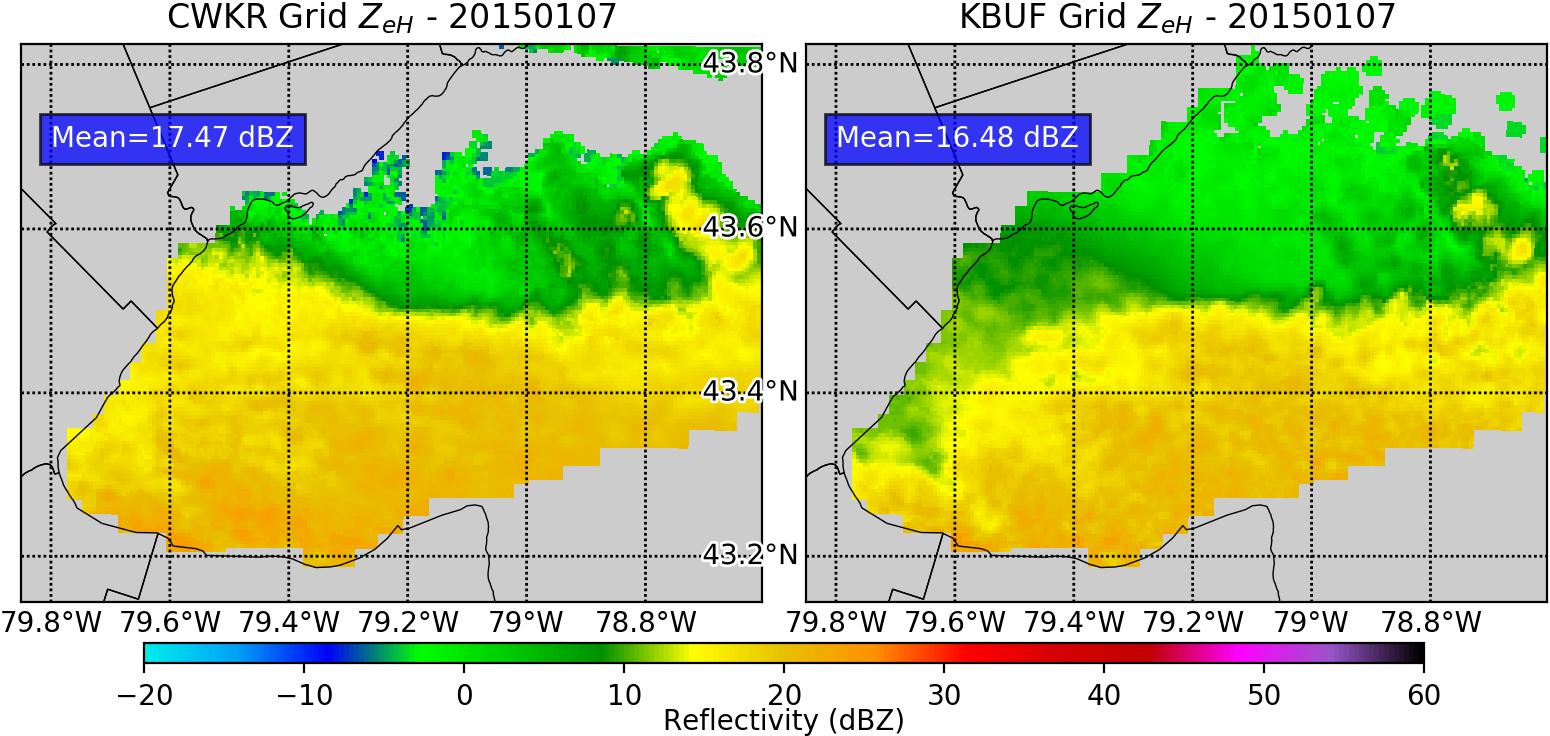
\includegraphics[width=\textwidth]{grid/ref/20150107}
\caption{Gridded $Z_{eH}$ comparison for 7 January 2015. Time-average of all admitted scans.} 
\label{fig:grid_ref_20150107}
\end{figure}

\begin{figure}[H]
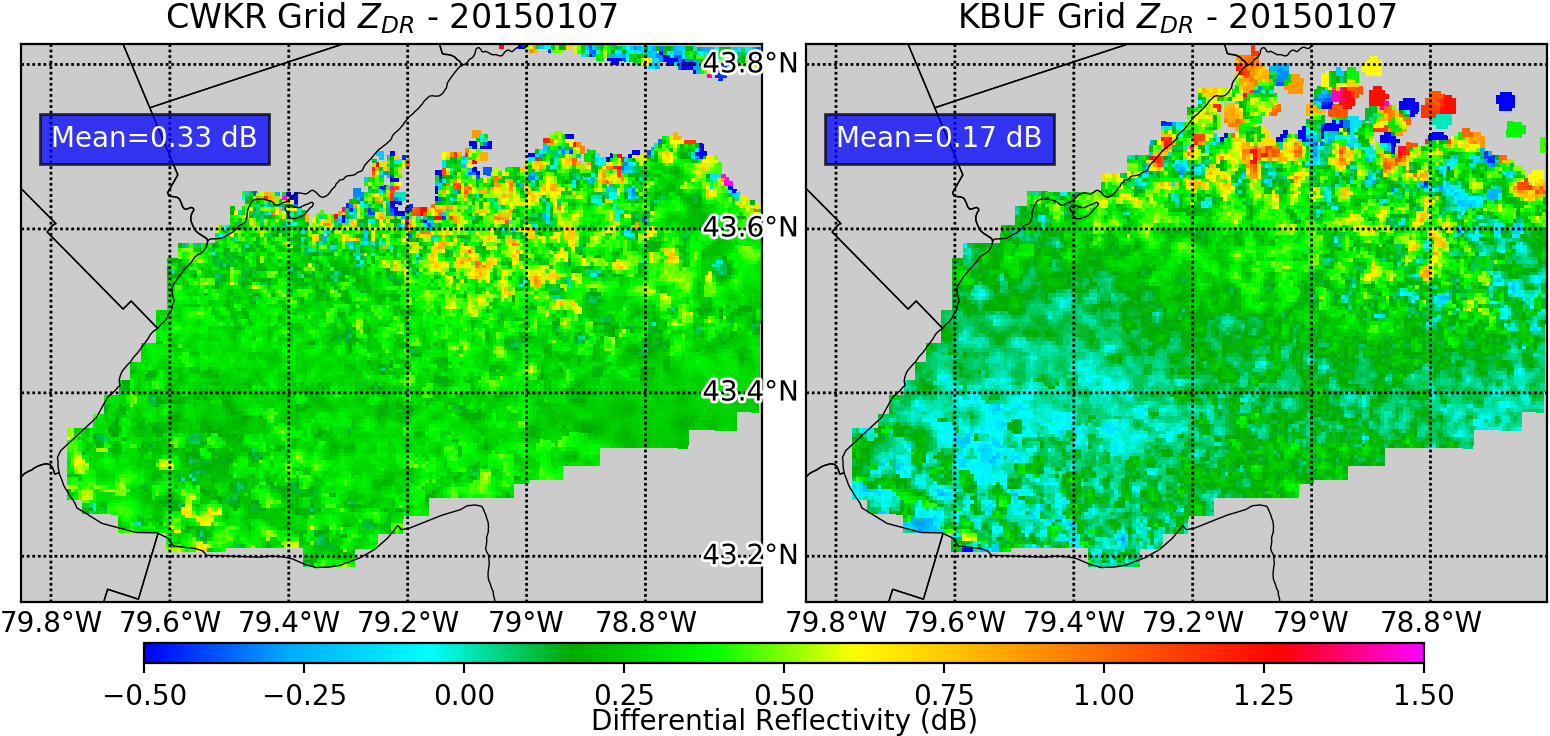
\includegraphics[width=\textwidth]{grid/zdr/20150107}
\caption{Gridded $Z_{DR}$ comparison for 7 January 2015. Time-average of all admitted scans.} 
\label{fig:grid_zdr_20150107}
\end{figure}
\begin{figure}[H]
\centering
   \begin{subfigure}{0.49\linewidth} \centering
     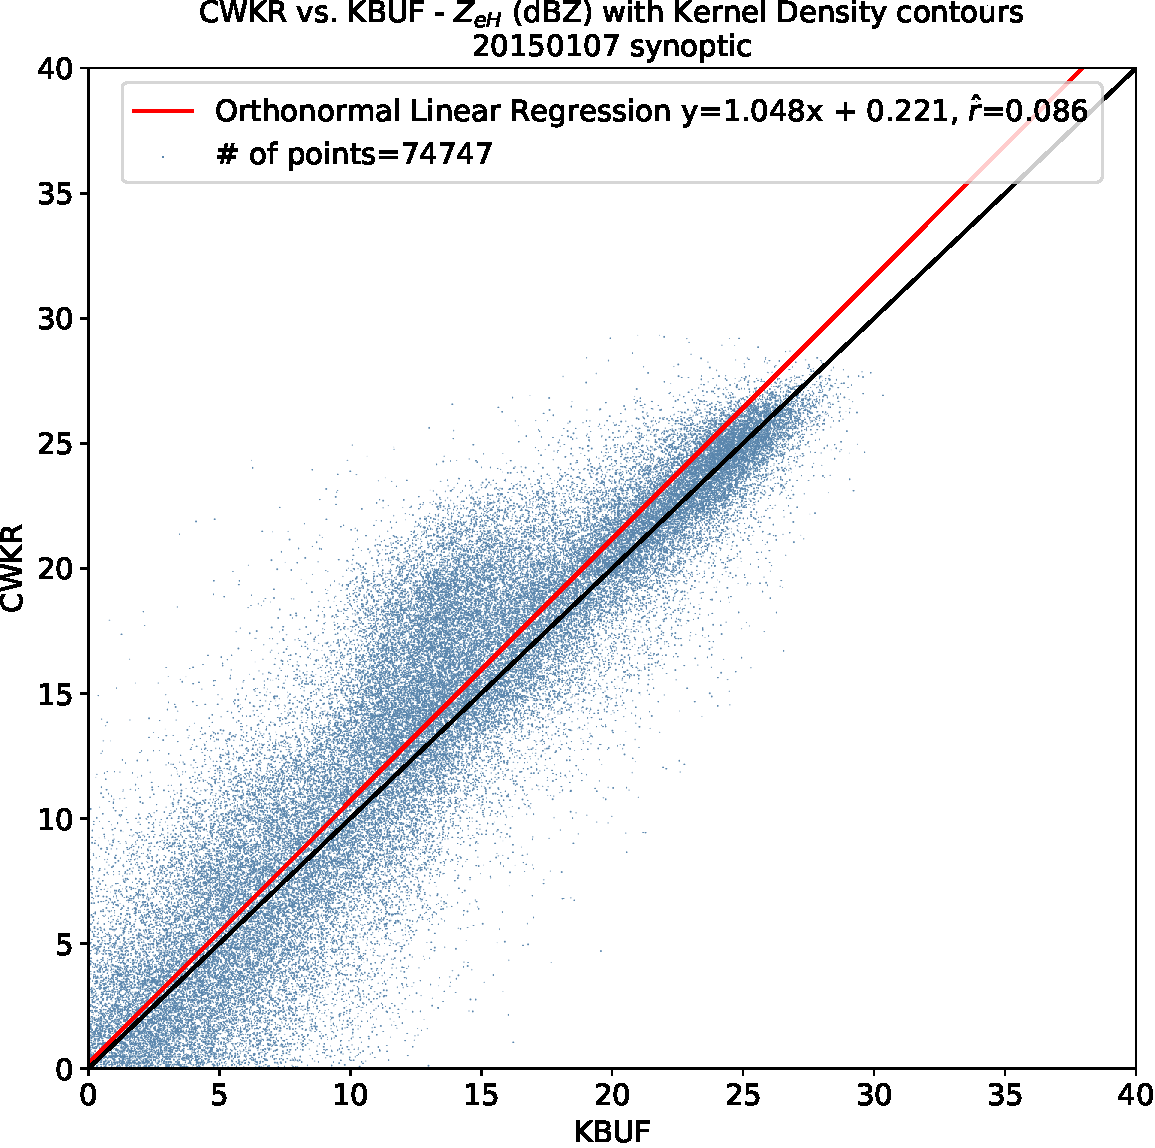
\includegraphics[scale=0.38]{scatter/ref/20150107}
     \caption{$Z_{eH}$ (dBZ)}\label{fig:scatter_ref_20150107}
   \end{subfigure}
   \begin{subfigure}{0.49\linewidth} \centering
     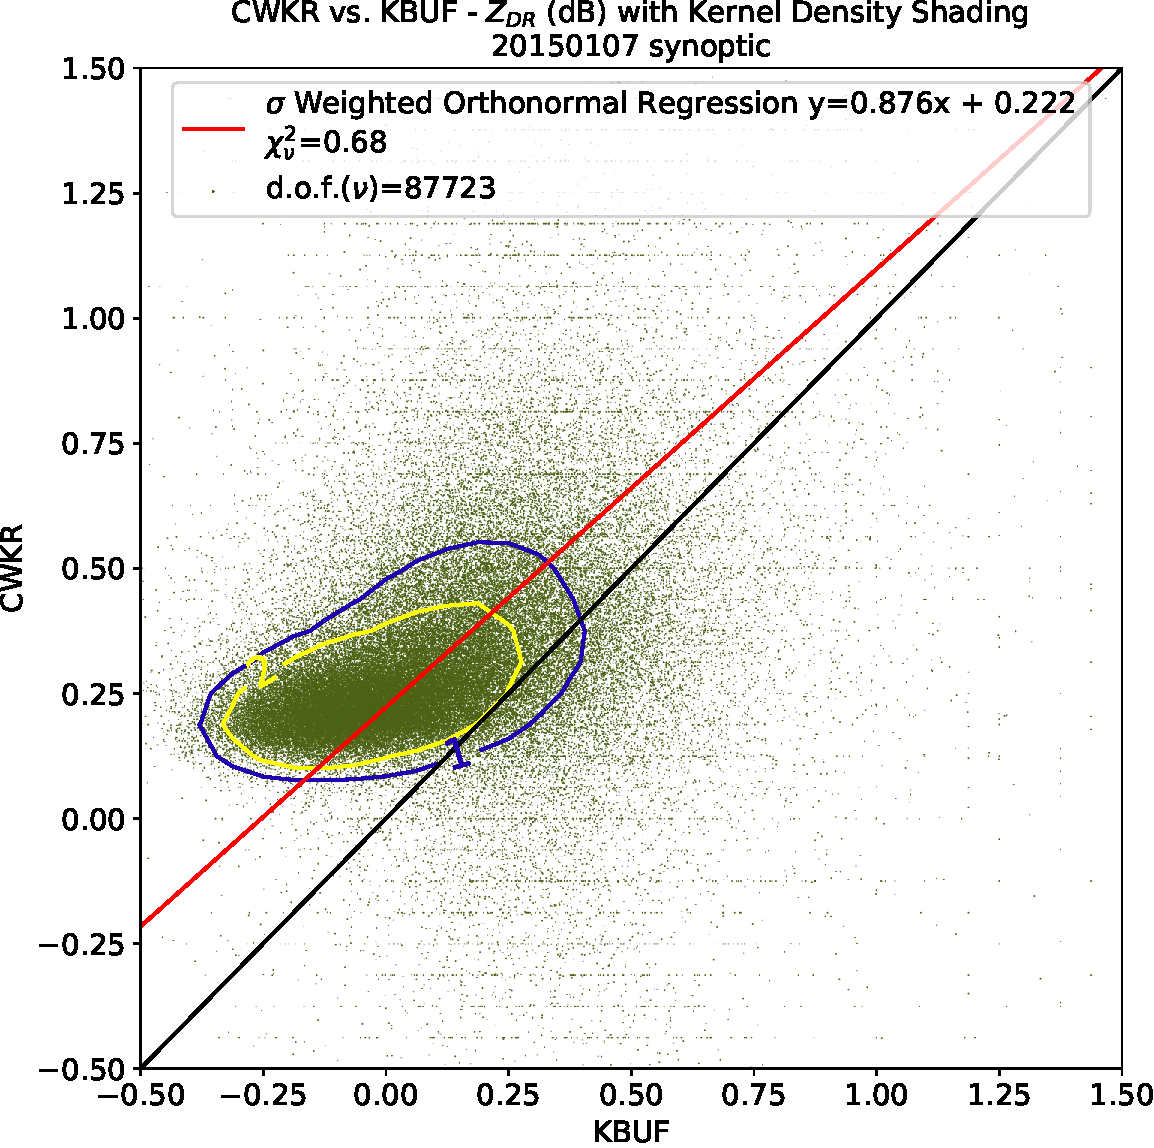
\includegraphics[scale=0.38]{scatter/zdr/20150107}
     \caption{$Z_{DR}$ (dB)}\label{fig:scatter_zdr_20150107}
   \end{subfigure}
\caption{Direct comparisons for 7 January 2015. Dataset includes all admitted grid cells.} \label{fig:scatter_20150107}
\end{figure}

\begin{figure}[H]
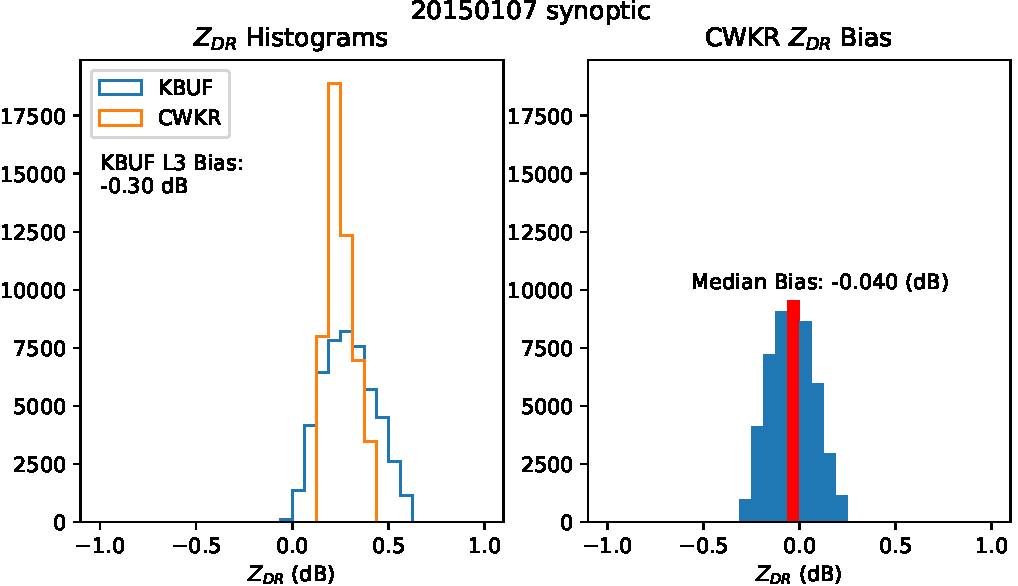
\includegraphics[width=0.75\textwidth]{hist/20150107}\centering
\caption{Histograms of $Z_{DR}$ (left), $Z_{DR}$ bias at CWKR, determined by subtracting the gridded, bias adjusted $Z_{DR}$ at KBUF from the $Z_{DR}$ at
CWKR. Both datasets include only matched points with KDE $\geq 2$. } 
\label{fig:hist_20150107}
\end{figure}

\subsection{6 February 2015 - Synoptic}
With a strong ridge centered over the SW US, Southern Ontario is on the backside of progressive shortwave, with a frontal passage occuring once again. A
broad swath of snow is depicted by the time-averaged $Z_{eH}$ fields in Figure \ref{fig:grid_ref_20150206}, with the CWKR mean value 2 dBZ higher than KBUF.
\begin{figure}[H]
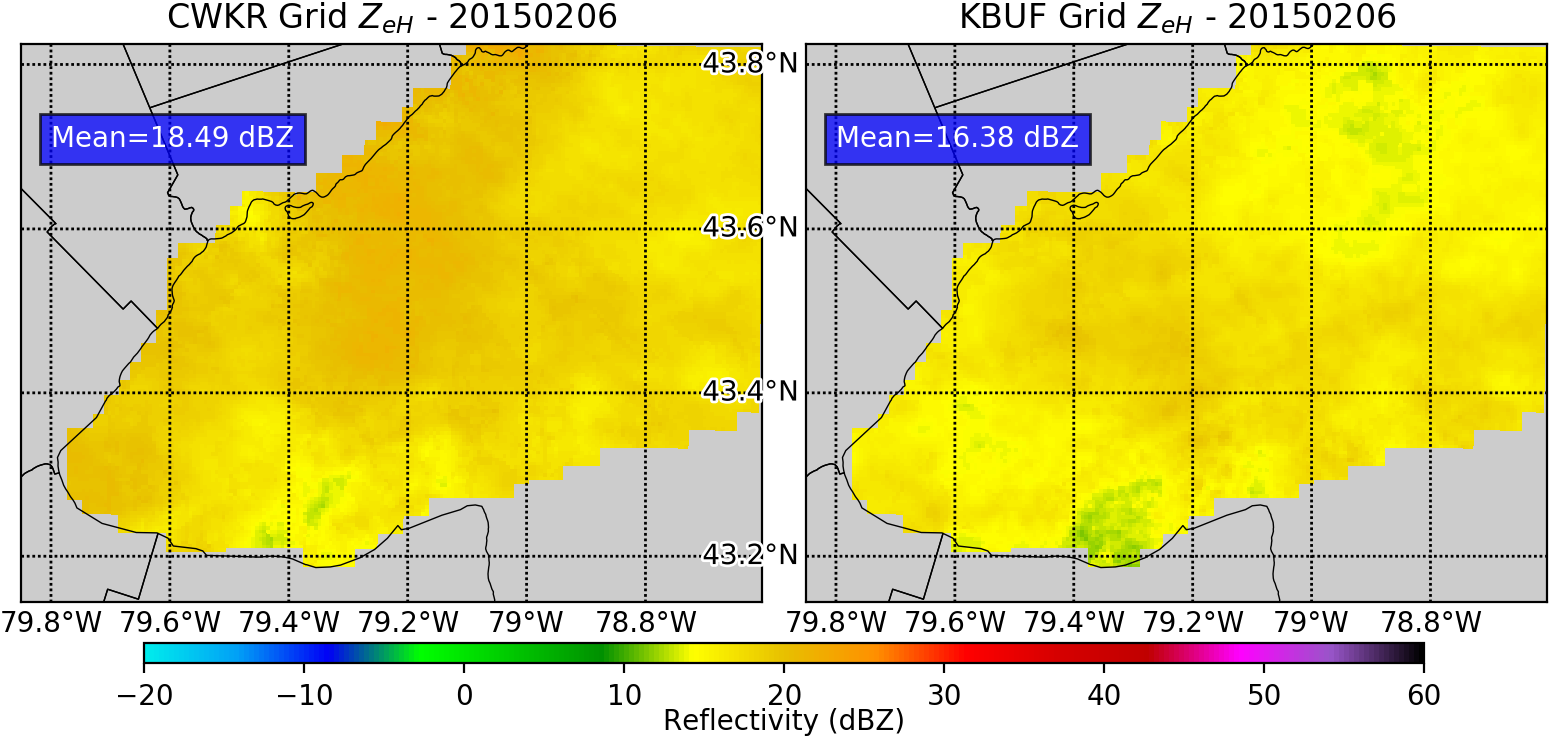
\includegraphics[width=\textwidth]{grid/ref/20150206}
\caption{Gridded $Z_{eH}$ comparison for 6 February 2015. Time-average of all admitted scans.} 
\label{fig:grid_ref_20150206}
\end{figure}
Comparing $Z_{DR}$ as shown in Figure \ref{fig:grid_zdr_20150206}, the fields are similiar but slightly biased. Beam blockages are noted at CWKR as indicated
by the stripes in the NE section of grid. Next to the scatter-plots, with Figure \ref{fig:scatter_20150206} indicating a high
frequency of points between 15-25 dBZ, a preferred range for comparing $Z_{DR}$ values. Also of note is the high error variance of 9.773 .
Figure \ref{fig:scatter_zdr_20150206} shows a dense, symmetric kernel with an ill-fitted regression. Proceeding on to the histograms in Figure
\ref{fig:hist_20150206}, a median bias of 0.283 dB at CWKR is estimated. The source of the bias will be discussed in the next chapter. 

\begin{figure}[p]
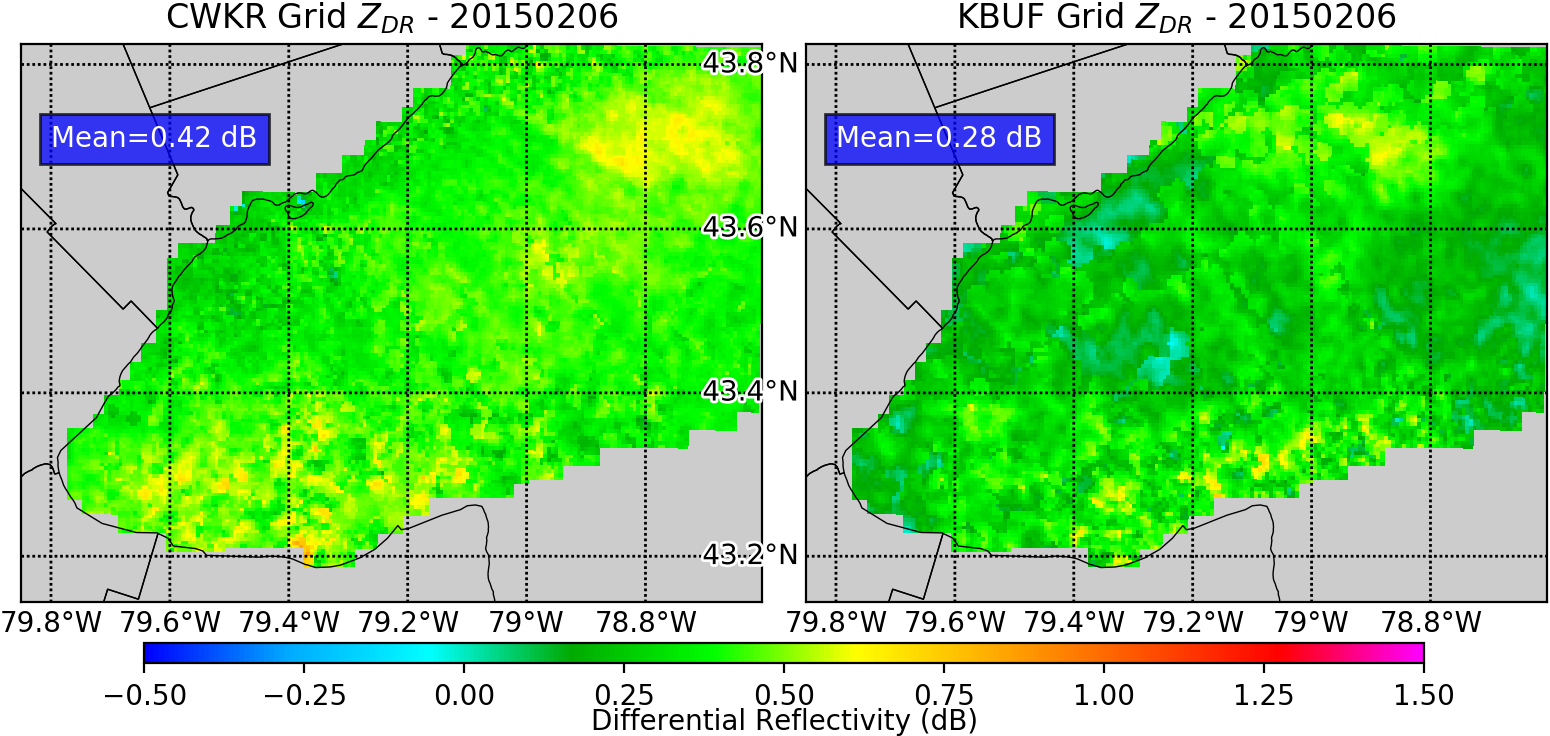
\includegraphics[width=\textwidth]{grid/zdr/20150206}
\caption{Gridded $Z_{DR}$ comparison for 6 February 2015. Time-average of all admitted scans.} 
\label{fig:grid_zdr_20150206}
\end{figure}

\begin{figure}[p]
\centering
   \begin{subfigure}{0.49\linewidth} \centering
     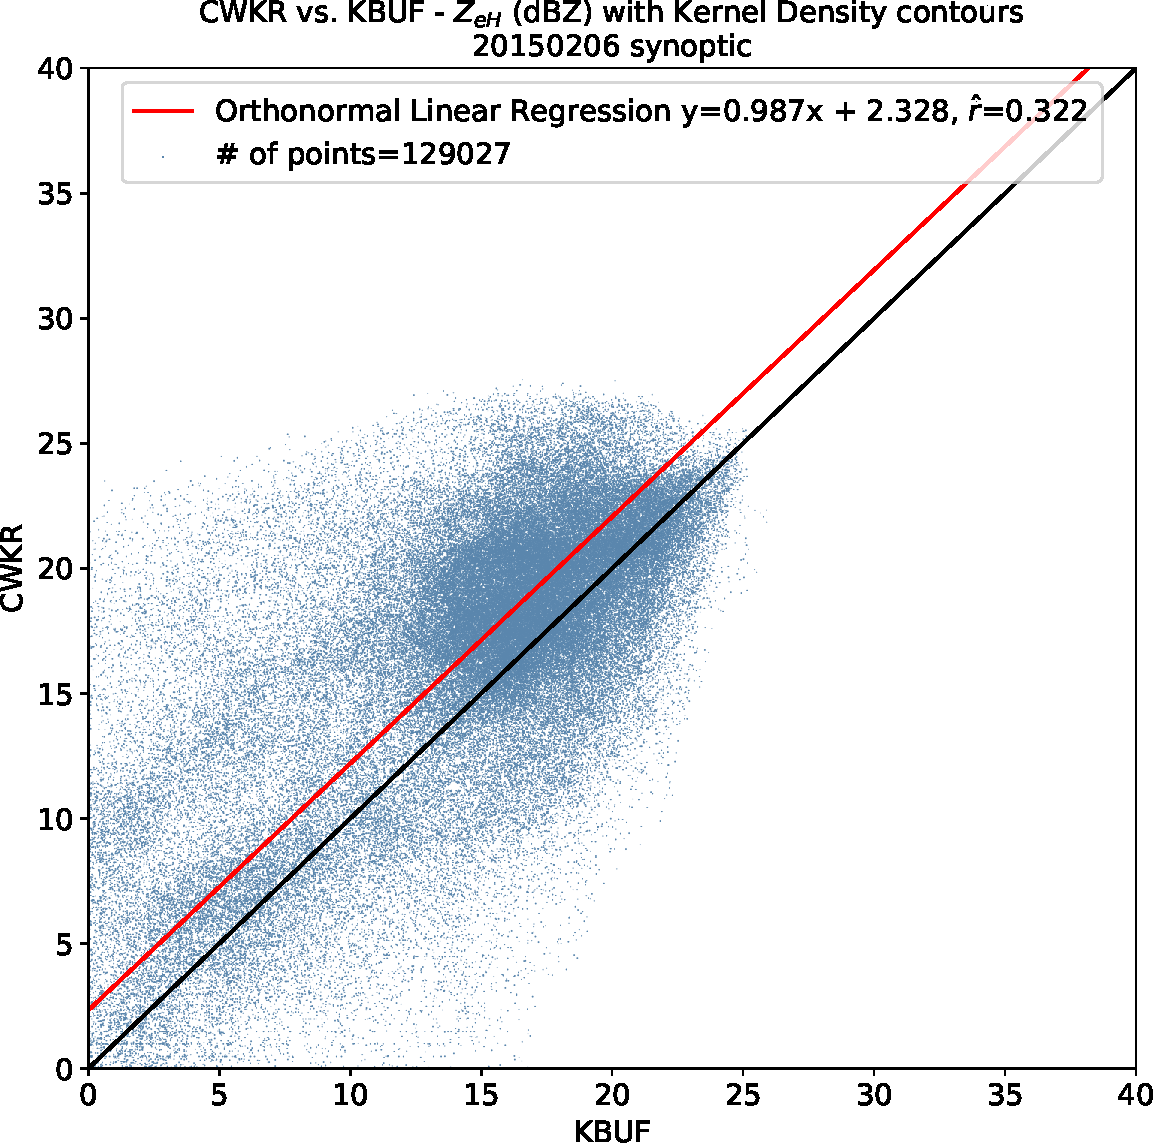
\includegraphics[scale=0.38]{scatter/ref/20150206}
     \caption{$Z_{eH}$ (dBZ)}\label{fig:scatter_ref_20150206}
   \end{subfigure}
   \begin{subfigure}{0.49\linewidth} \centering
     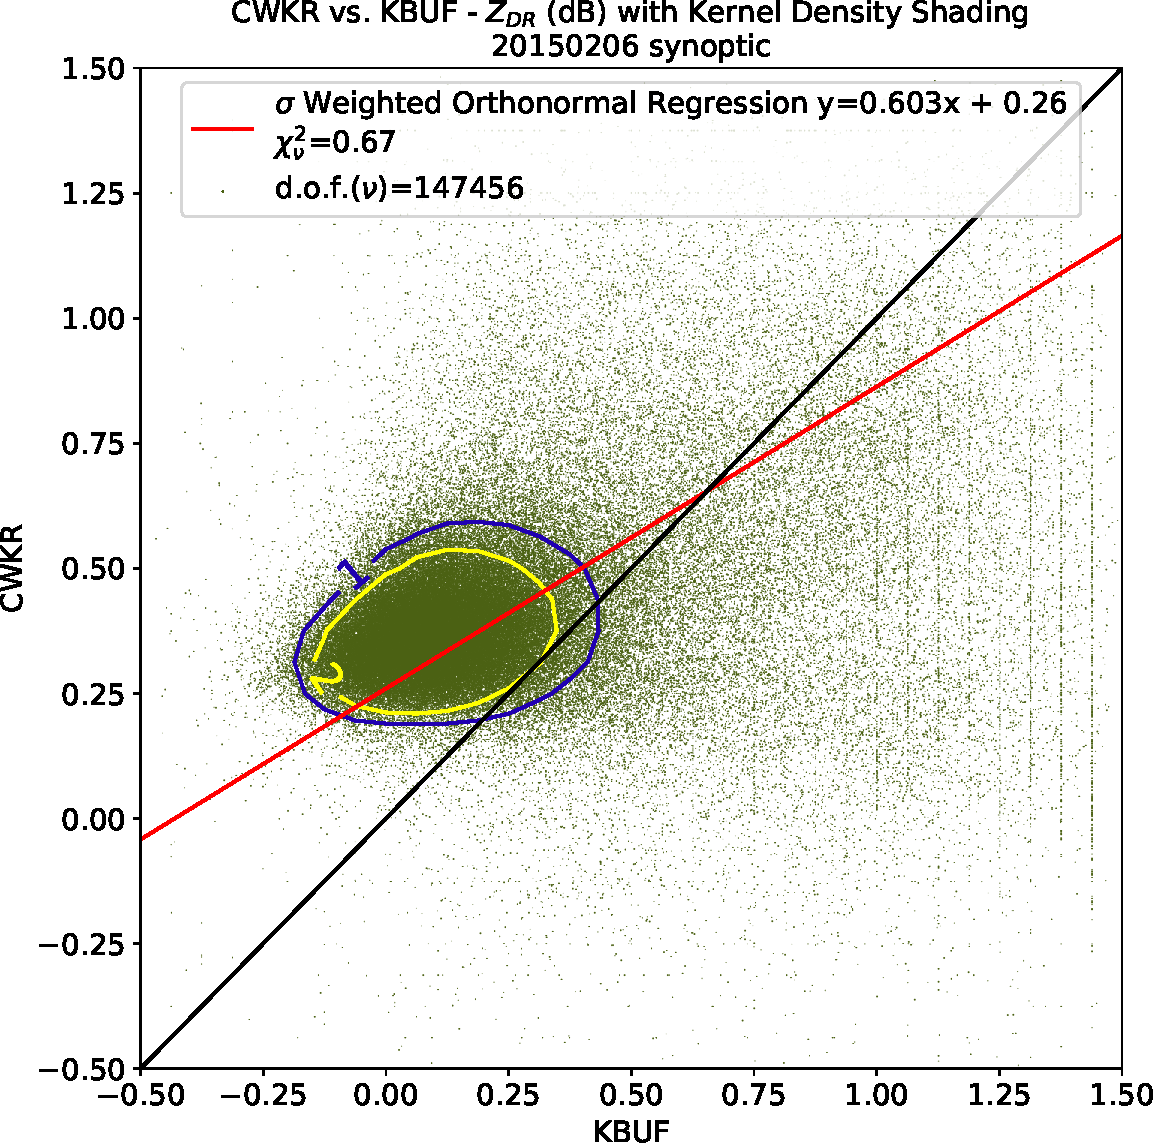
\includegraphics[scale=0.38]{scatter/zdr/20150206}
     \caption{$Z_{DR}$ (dB)}\label{fig:scatter_zdr_20150206}
   \end{subfigure}
\caption{Direct comparisons for 6 February 2015. Dataset includes all admitted grid cells.} \label{fig:scatter_20150206}
\end{figure}

\begin{figure}[H]
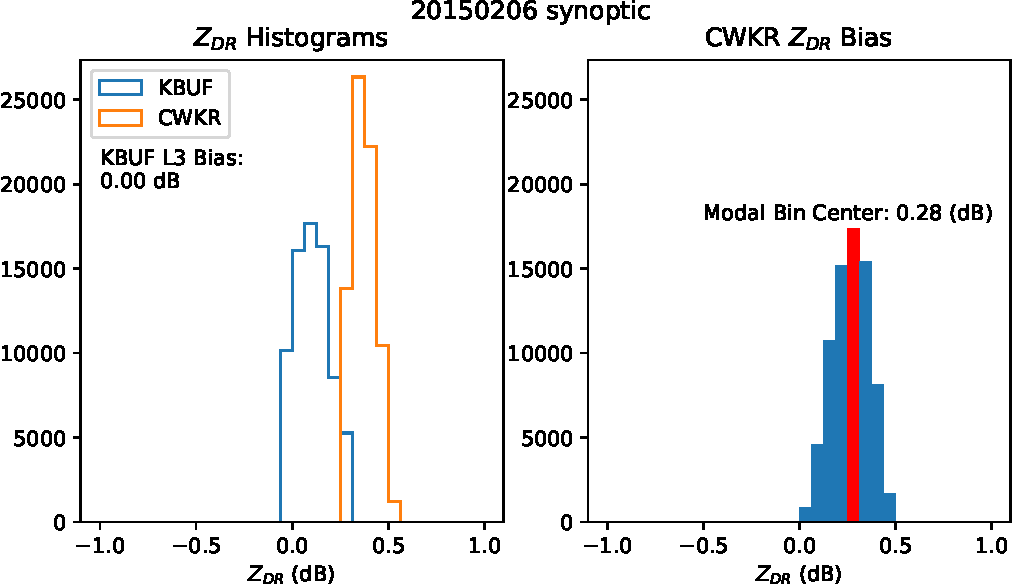
\includegraphics[width=0.75\textwidth]{hist/20150206}\centering
\caption{Histograms of $Z_{DR}$ (left), $Z_{DR}$ bias at CWKR, determined by subtracting the gridded, bias adjusted $Z_{DR}$ at KBUF from the $Z_{DR}$ at
CWKR. Both datasets include only matched points with KDE $\geq 2$. } 
\label{fig:hist_20150206}
\end{figure}

\subsection{14 February 2015 - Lake-Effect}
While Southern Ontario is bracing for the impact of a bowling-ball like lobe of the polar vortex, strong W to SW flow from the surface to 850mb allows for a prolonged period of lake-effect snow over the lake. From Figure \ref{fig:grid_ref_20150214}, we see again that CWKR resolves the convective scale features of the snow squalls better than KBUF. Horizontal convective rolls are clearly depicted by CWKR, whereas they become muddled by KBUF. Figure \ref{fig:grid_zdr_20150214} shows similiar patterns of $Z_{DR}$, but a large bias exists. The $Z_{eH}$ scatter-plot in Figure \ref{fig:scatter_20150214} shows a dense clustering of points for low values, becoming increasingly skewed towards CWKR as they increase. For $Z_{DR}$, the variance-weighted regression achieves a near perfect reduced chi statistic ($\chi^2_\nu$) of 0.968. The histogram in Figure \ref{fig:hist_20150214} indicates a anomalous bias for this event, with a median value of 0.377 dB.

\begin{figure}[p]
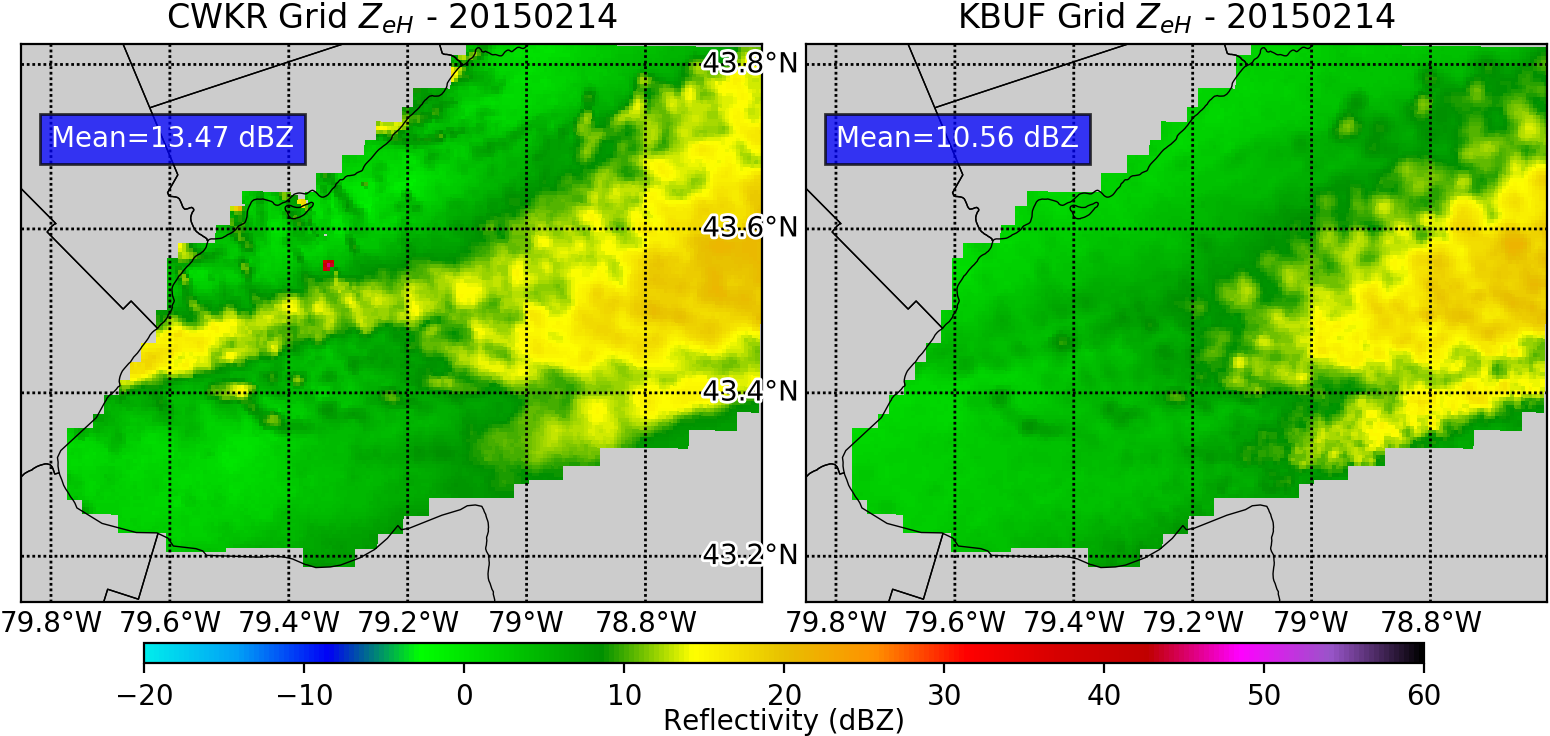
\includegraphics[width=\textwidth]{grid/ref/20150214}
\caption{Gridded $Z_{eH}$ comparison for 14 February 2015. Time-average of all admitted scans.} 
\label{fig:grid_ref_20150214}
\end{figure}

\begin{figure}[p]
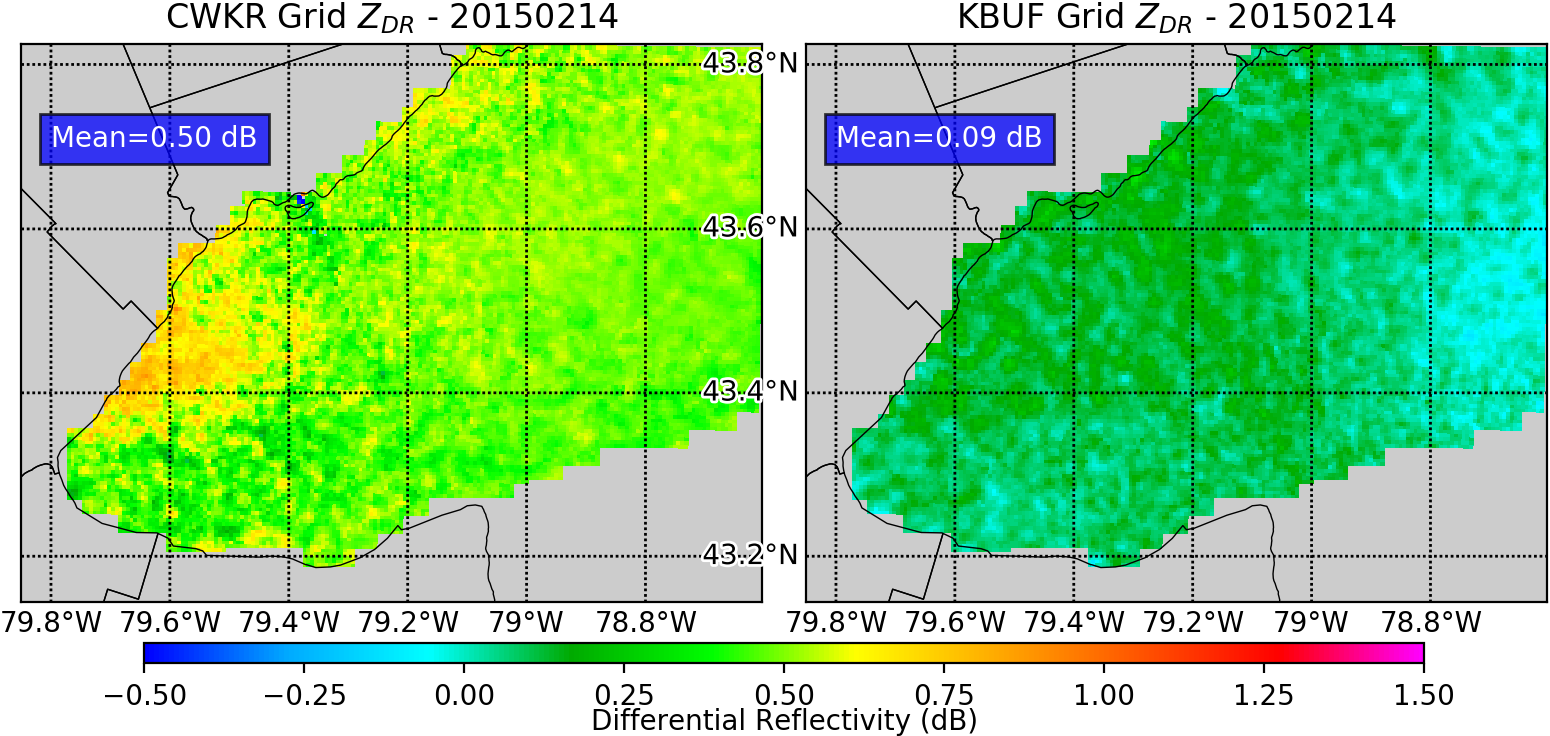
\includegraphics[width=\textwidth]{grid/zdr/20150214}
\caption{Gridded $Z_{DR}$ comparison for 14 February 2015. Time-average of all admitted scans.} 
\label{fig:grid_zdr_20150214}
\end{figure}

\begin{figure}[p]
\centering
   \begin{subfigure}{0.49\linewidth} \centering
     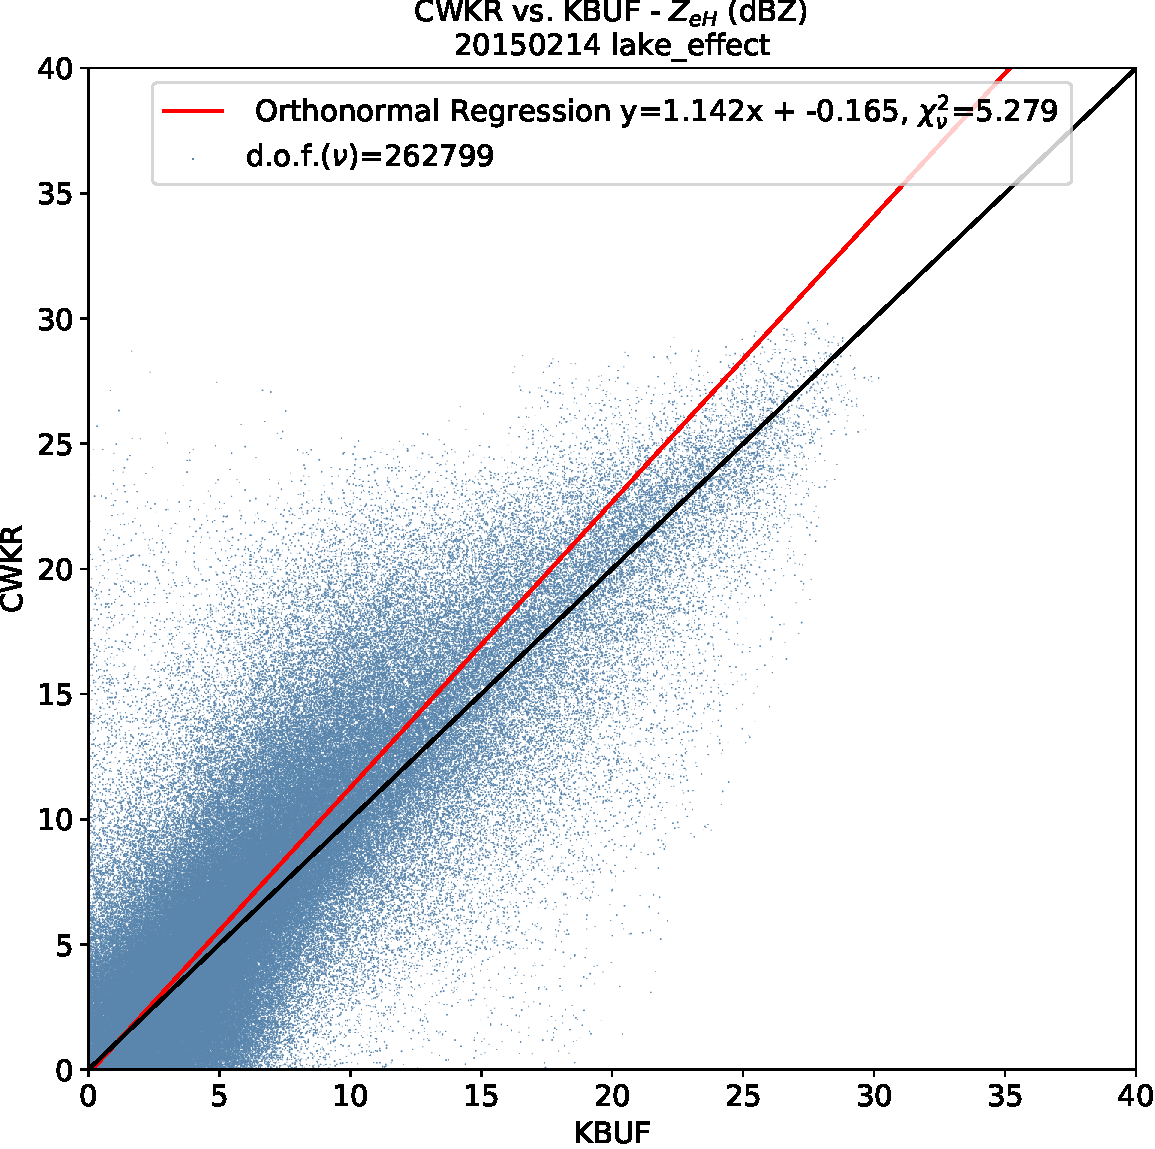
\includegraphics[scale=0.38]{scatter/ref/20150214}
     \caption{$Z_{eH}$ (dBZ)}\label{fig:scatter_ref_20150214}
   \end{subfigure}
   \begin{subfigure}{0.49\linewidth} \centering
     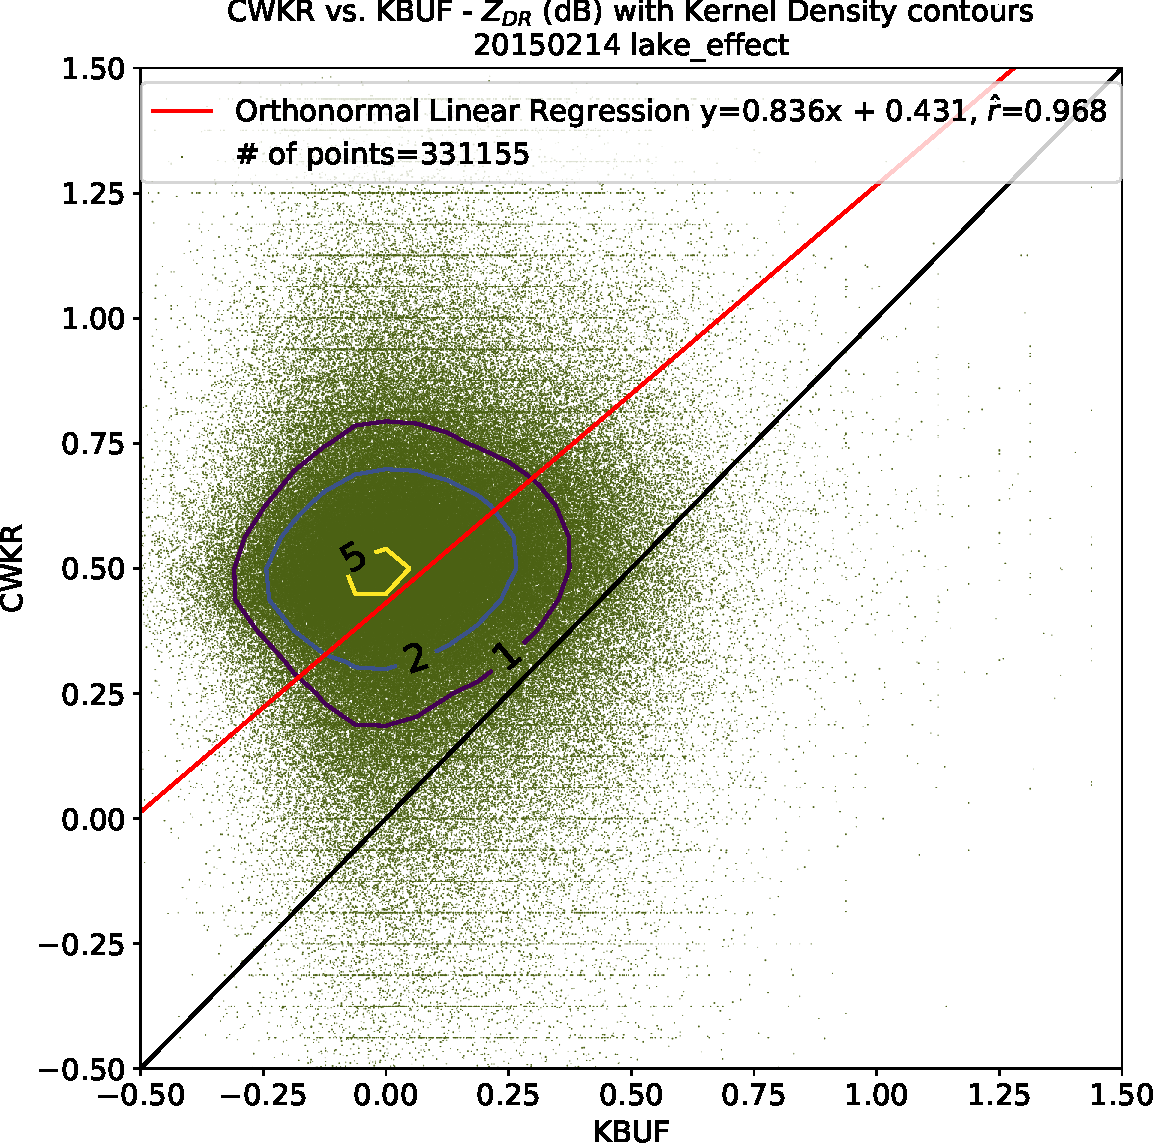
\includegraphics[scale=0.38]{scatter/zdr/20150214}
     \caption{$Z_{DR}$ (dB)}\label{fig:scatter_zdr_20150214}
   \end{subfigure}
\caption{Direct comparisons for 14 February 2015. Dataset includes all admitted grid cells.} \label{fig:scatter_20150214}
\end{figure}

\begin{figure}[p]
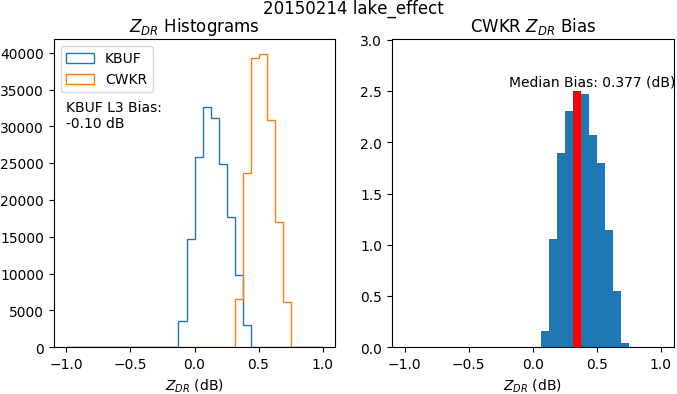
\includegraphics[width=0.75\textwidth]{hist/20150214}\centering
\caption{Histograms of $Z_{DR}$ (left), $Z_{DR}$ bias at CWKR, determined by subtracting the gridded, bias adjusted $Z_{DR}$ at KBUF from the $Z_{DR}$ at CWKR. Both datasets include only matched points with KDE $\geq 2$. } 
\label{fig:hist_20150214}
\end{figure}

\subsection{18 February 2015 - Lake-Effect}
Four days later, The polar vortex has arrived in earnest for this event, with the 500 dm isoheight at 500mb nearing as far south as Windsor, ON. The cold airmass allows for the development of an intense lake-effect snow band, the strongest of all the lake-effect cases as indicated by the $Z_{eH}$ means in Figure \ref{fig:grid_ref_20150218}. Next, Figure \ref{fig:grid_zdr_20150218} shows similiar band structure as compared between radars, with a bias evident. A orthonormal fit with decent agreement between radars is shown in Figure \ref{fig:scatter_ref_20150218}, with the values biased towards CWKR all along the line. In Figure \ref{fig:scatter_zdr_20150218}, a unique bi-modal distribution of $Z_{DR}$ is shown, with two peaks equal in magnitude around 0.50 dB and 0.75 dB. The histogram in Figure \ref{fig:hist_20150218} also depicts this bi-modal distribution of $Z_{DR}$, and gives an estimate median value of 0.296 dB. The source of the bias will be discussed in the next chapter. 
\begin{figure}[H]
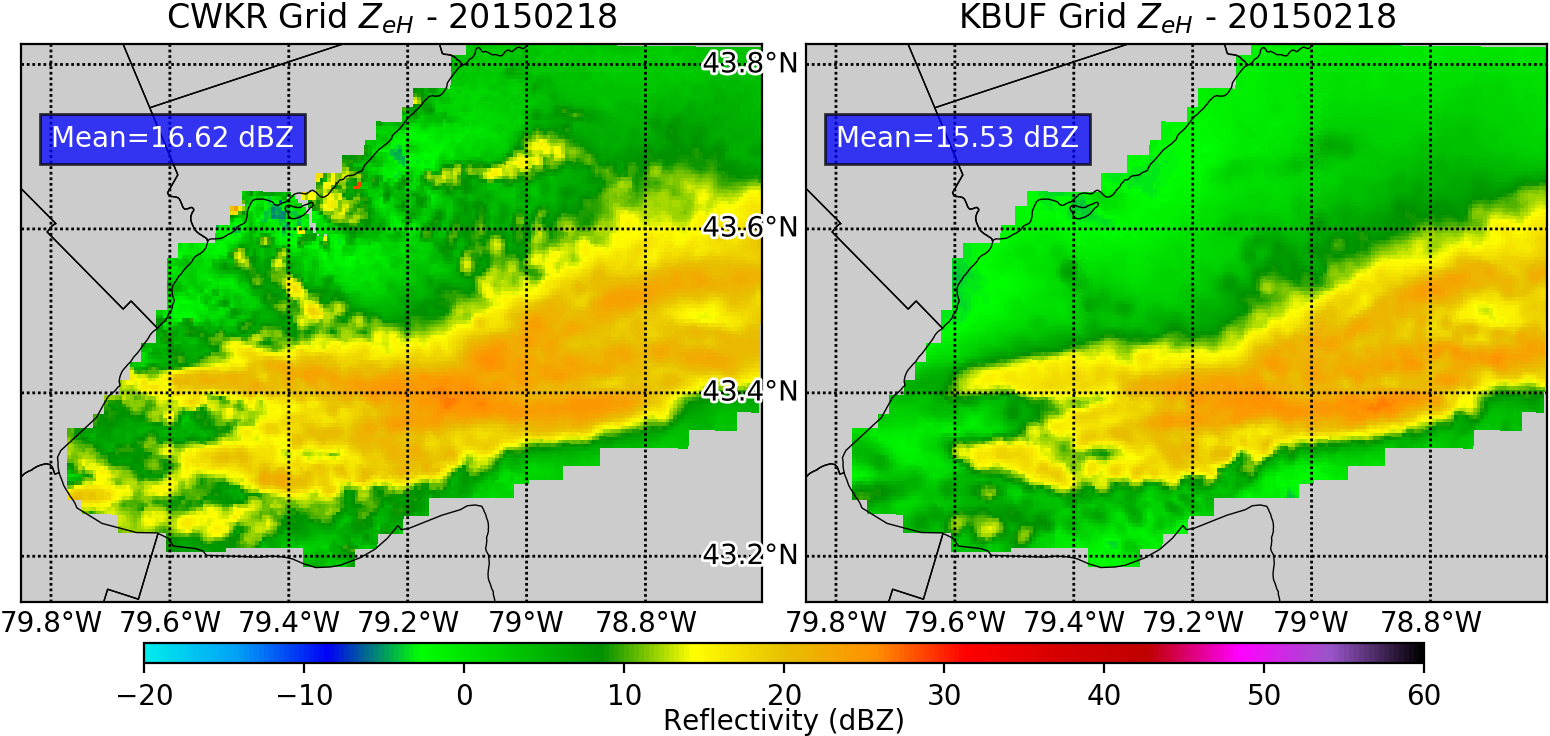
\includegraphics[width=\textwidth]{grid/ref/20150218}
\caption{Gridded $Z_{eH}$ comparison for 18 February 2015. Time-average of all admitted scans.} 
\label{fig:grid_ref_20150218}
\end{figure}

\begin{figure}[p]
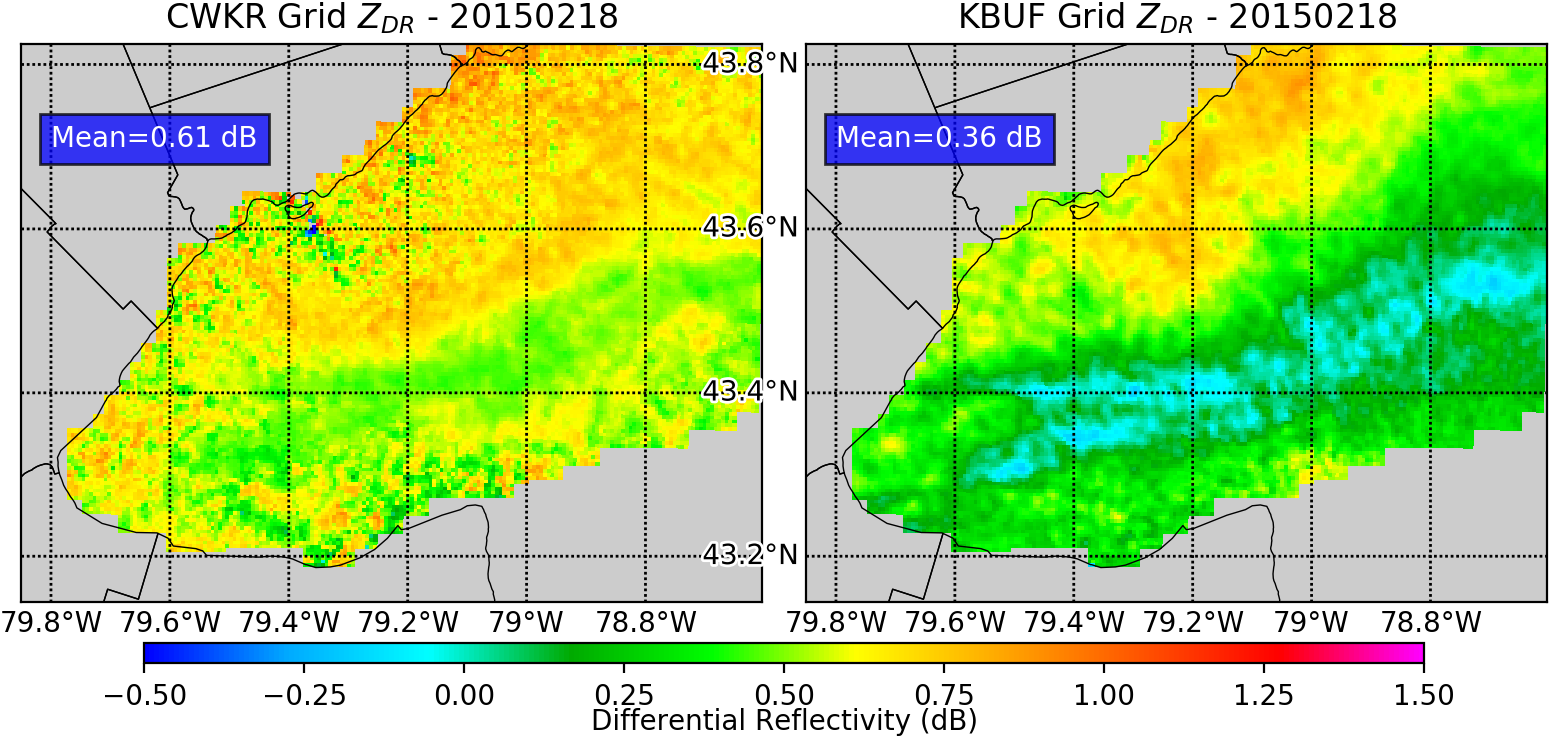
\includegraphics[width=\textwidth]{grid/zdr/20150218}
\caption{Gridded $Z_{DR}$ comparison for 18 February 2015. Time-average of all admitted scans.} 
\label{fig:grid_zdr_20150218}
\end{figure}

\begin{figure}[p]
\centering
   \begin{subfigure}{0.49\linewidth} \centering
     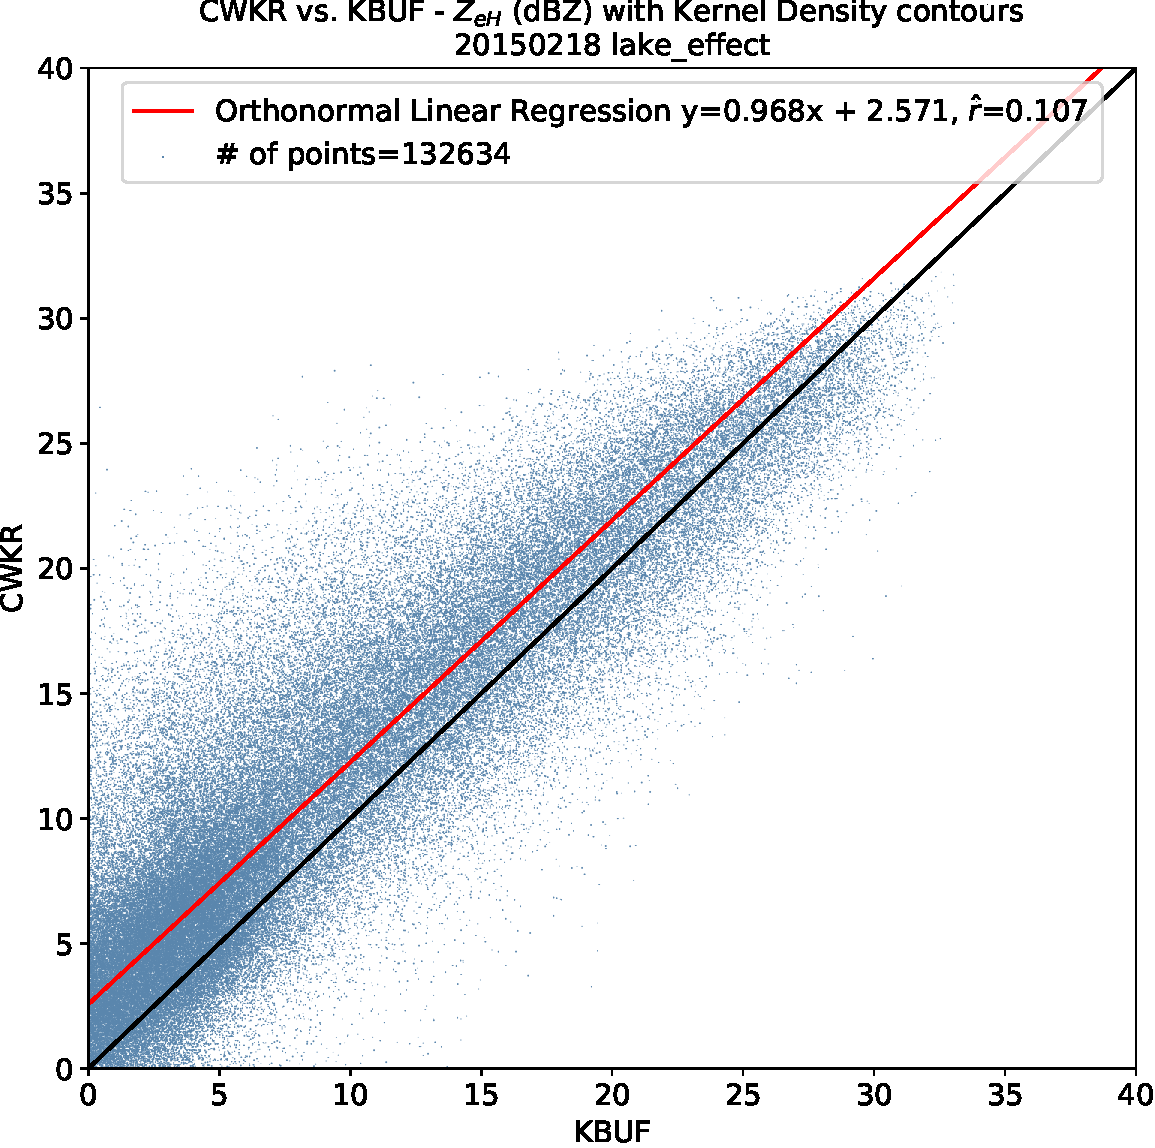
\includegraphics[scale=0.38]{scatter/ref/20150218}
     \caption{$Z_{eH}$ (dBZ)}\label{fig:scatter_ref_20150218}
   \end{subfigure}
   \begin{subfigure}{0.49\linewidth} \centering
     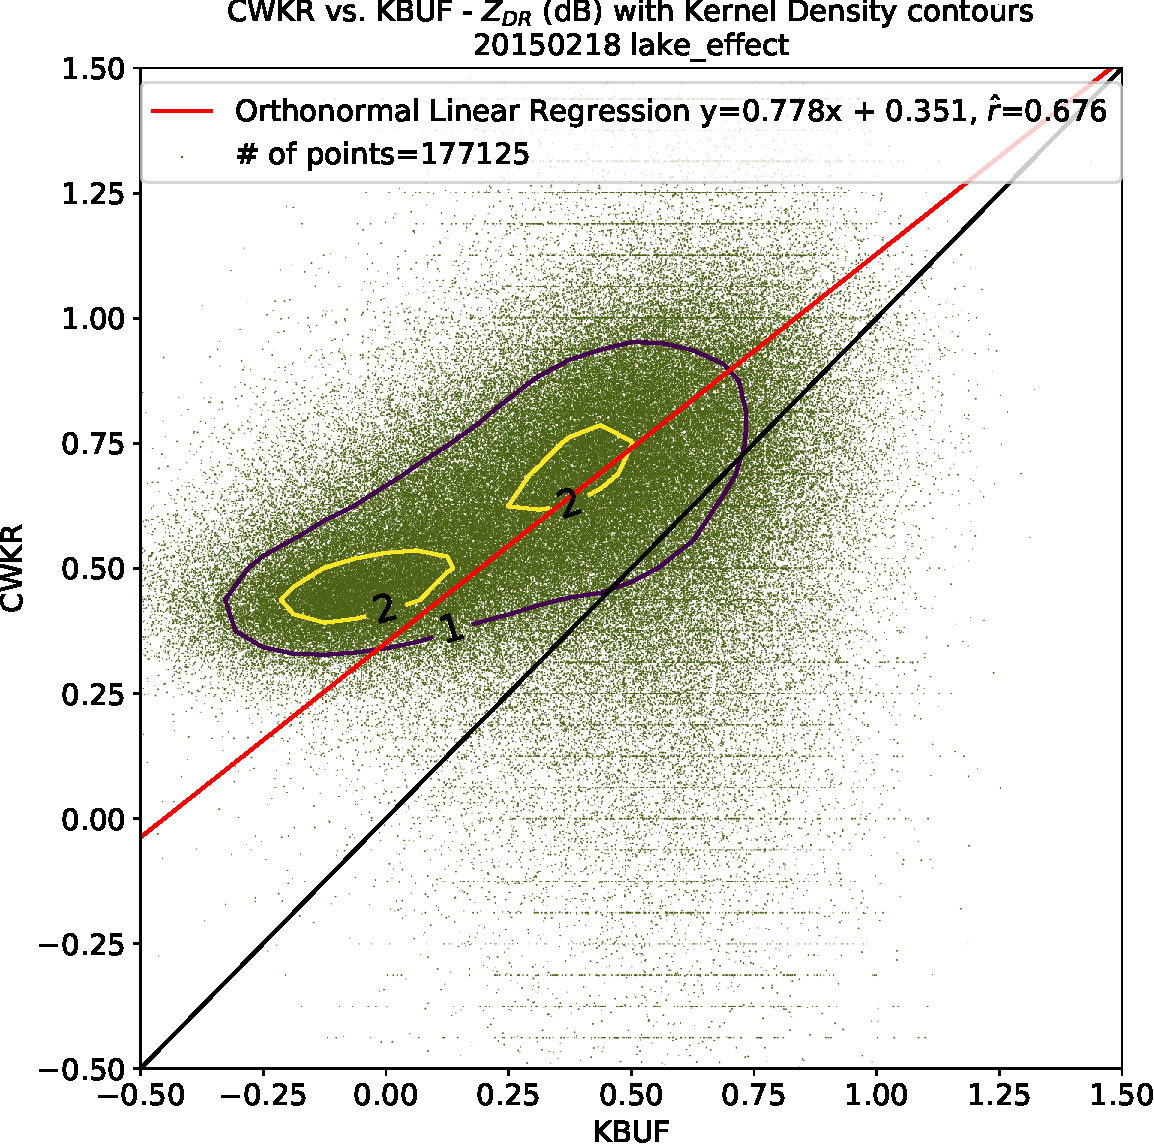
\includegraphics[scale=0.38]{scatter/zdr/20150218}
     \caption{$Z_{DR}$ (dB)}\label{fig:scatter_zdr_20150218}
   \end{subfigure}
\caption{Direct comparisons for 18 February 2015. Dataset includes all admitted grid cells.} \label{fig:scatter_20150218}
\end{figure}

\begin{figure}[H]
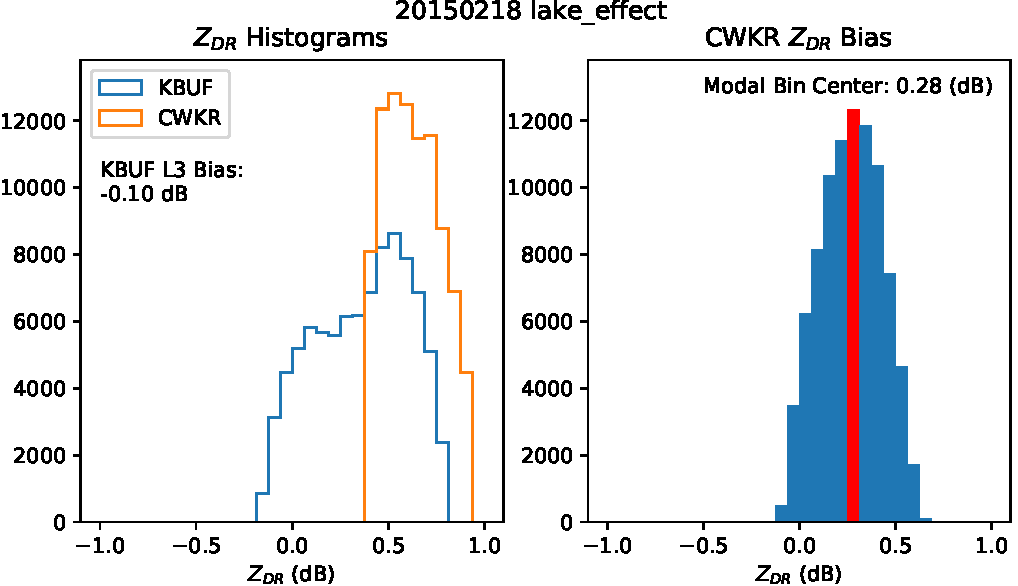
\includegraphics[width=0.75\textwidth]{hist/20150218}\centering
\caption{Histograms of $Z_{DR}$ (left), $Z_{DR}$ bias at CWKR, determined by subtracting the gridded, bias adjusted $Z_{DR}$ at KBUF from the $Z_{DR}$ at
CWKR. Both datasets include only matched points with KDE $\geq 2$. } 
\label{fig:hist_20150218}
\end{figure}

\subsection{10 February 2016 - Lake-Effect}
The 500mb ridge axis is centered to the south of Southern Ontario in the Appalachians, with WNW flow aloft during this event. With a slight amount of pre
existing instability augmenting the lake induced instabilities, a healthly band of lake-effect snow forms on the southern end of the lake. KBUF observes
higher values of $Z_{DR}$ in this band on the southern edge of the lake, as shown in Figure \ref{fig:grid_ref_20160210}. This is likely due to the CWKR beam
overshooting the shallow convection while the KBUF beam is lower in height. The intensity of the band overcomes the degraded signal strength due beam
blockages at CWKR, evident in $Z_{DR}$ on the western end of the band in Figure \ref{fig:grid_zdr_20160210}. 
\begin{figure}[H]
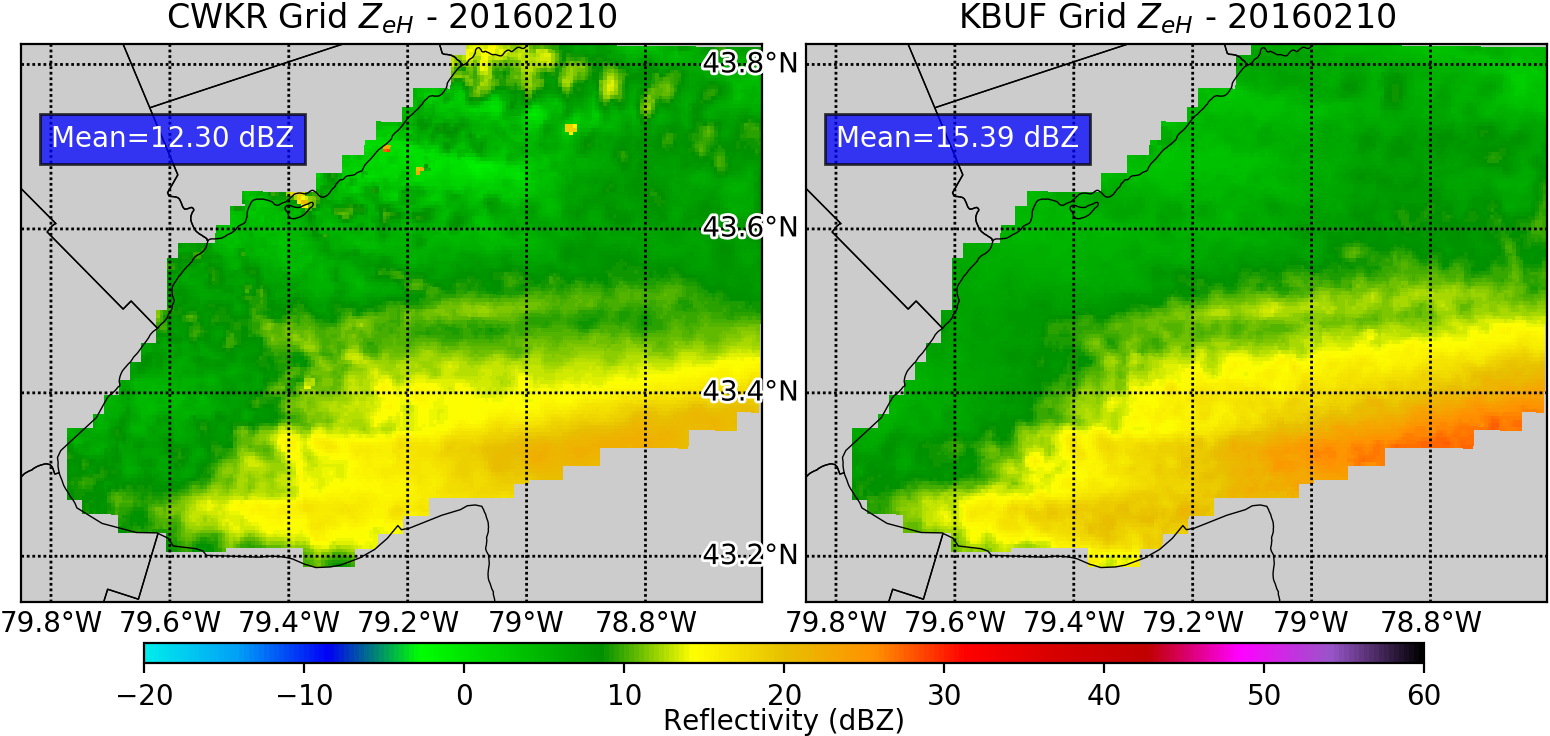
\includegraphics[width=\textwidth]{grid/ref/20160210}
\caption{Gridded $Z_{eH}$ comparison for 10 February 2016. Time-average of all admitted scans.} 
\label{fig:grid_ref_20160210}
\end{figure}

\begin{figure}[H]
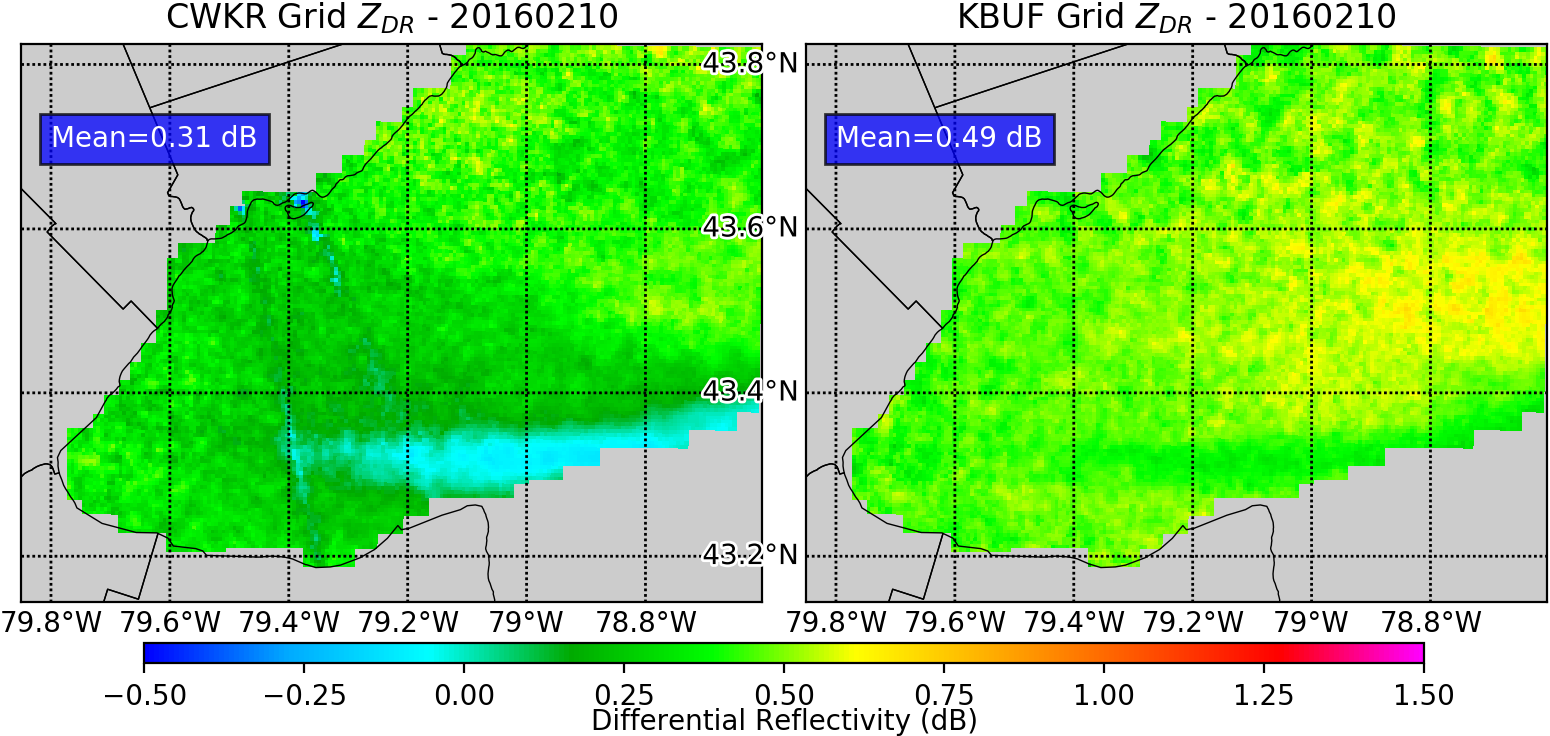
\includegraphics[width=\textwidth]{grid/zdr/20160210}
\caption{Gridded $Z_{DR}$ comparison for 10 February 2016. Time-average of all admitted scans.} 
\label{fig:grid_zdr_20160210}
\end{figure}

\vspace{5mm}

Due to the long duration of this case, the large
sample of matched points was obtained from this case. Figure \ref{fig:scatter_ref_20160210} shows that matched $Z_{eH}$ values tends higher towards KBUF as
they increase. Next, Figure \ref{fig:scatter_zdr_20160210} demonstrates the value of the kernel density estimate, as its impossible to visually analyze a
scatter-plot with nearly a million points. The kernel extracted from the data is small, but information rich. Figure \ref{fig:hist_20160210} leverages this
information to show that the median $Z_{DR}$ at CWKR is -0.055 dB, indicating no discernible bias exists outside of the error threshold of $\pm$0.1 dB for
this event.

\begin{figure}[H]
\centering
   \begin{subfigure}{0.49\linewidth} \centering
     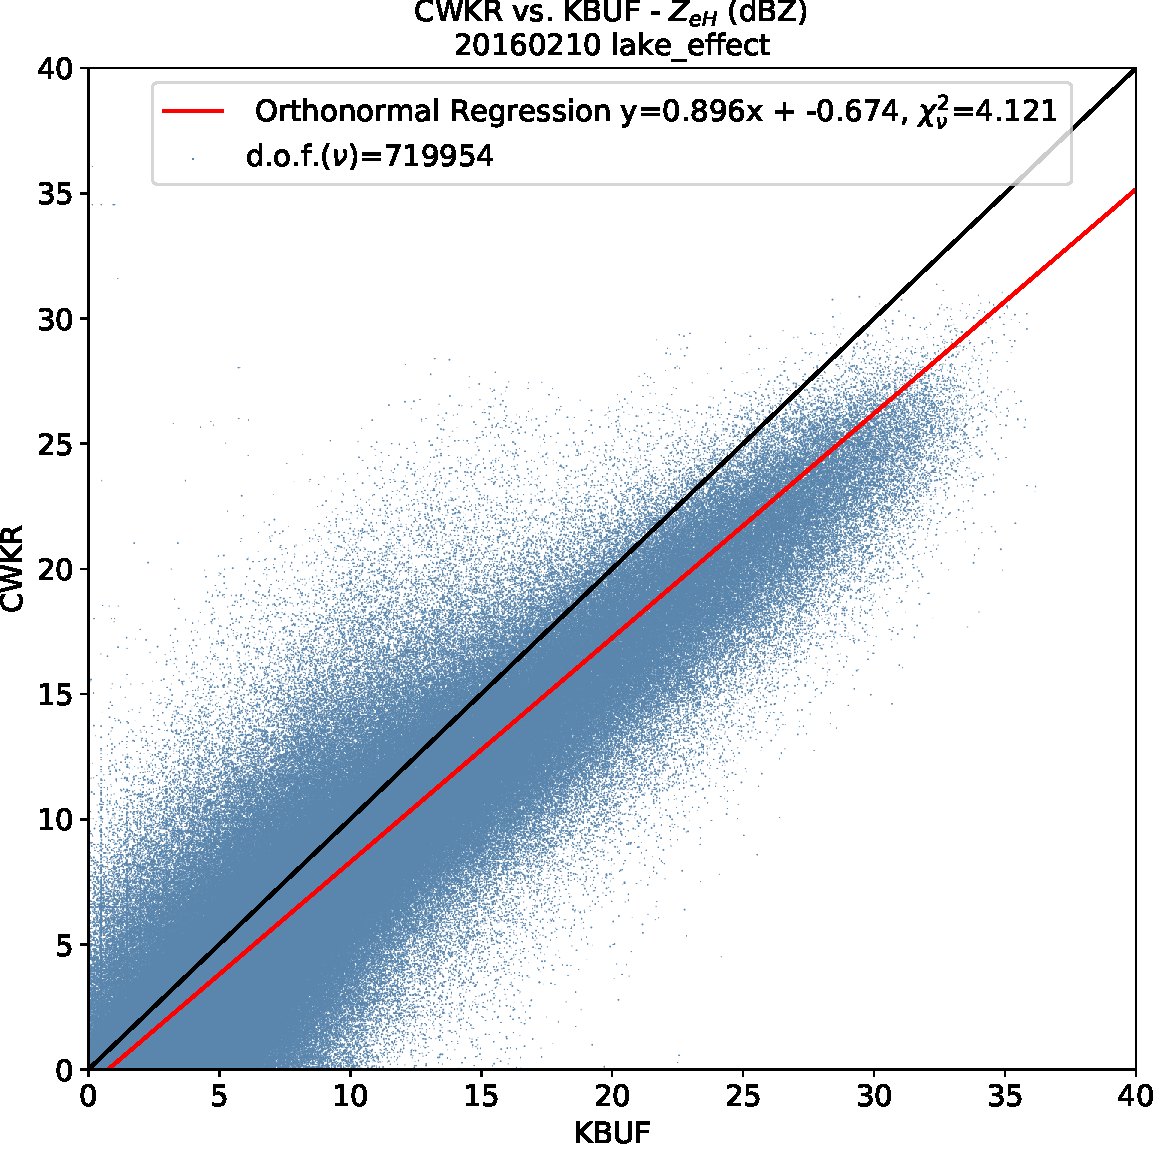
\includegraphics[scale=0.38]{scatter/ref/20160210}
     \caption{$Z_{eH}$ (dBZ)}\label{fig:scatter_ref_20160210}
   \end{subfigure}
   \begin{subfigure}{0.49\linewidth} \centering
     \includegraphics[scale=0.38]{scatter/zdr/20160210}
     \caption{$Z_{DR}$ (dB)}\label{fig:scatter_zdr_20160210}
   \end{subfigure}
\caption{Direct comparisons for 10 February 2016. Dataset includes all admitted grid cells.} \label{fig:scatter_20160210}
\end{figure}

\begin{figure}[H]
\includegraphics[width=0.75\textwidth]{hist/20160210}\centering
\caption{Histograms of $Z_{DR}$ (left), $Z_{DR}$ bias at CWKR, determined by subtracting the gridded, bias adjusted $Z_{DR}$ at KBUF from the $Z_{DR}$ at
CWKR. Both datasets include only matched points with KDE $\geq 2$. } 
\label{fig:hist_20160210}
\end{figure}

\subsection{15 December 2016 - Synoptic}
A deep longwave trough is centered over Southern Ontario, with an Arctic airmass in place over the Great Lakes region. With meager moisture in place, a
post-frontal trough manages to squeeze out some passing snow-showers. As indicated by Figure \ref{fig:grid_ref_20161215}, the spatial patterns of $Z_{eH}$ are in very good agreement. In contrast, Figure \ref{fig:grid_zdr_20161215} shows two very noisy $Z_{DR}$ fields. Even with the small sample size, Figure \ref{fig:scatter_20161215} shows that decent fits are achieved for both moments. Meanwhile, the histogram in Figure \ref{fig:hist_20161215} shows that the estimate of bias at CWKR is large, with a median value of -0.465 dB. This case is an outlier; the source of this large bias will be discussed in the next chapter. 
\begin{figure}[p]
\includegraphics[width=\textwidth]{grid/ref/20161215}
\caption{Gridded $Z_{eH}$ comparison for 15 December 2016. Time-average of all admitted scans.} 
\label{fig:grid_ref_20161215}
\end{figure}

\begin{figure}[p]
\includegraphics[width=\textwidth]{grid/zdr/20161215}
\caption{Gridded $Z_{DR}$ comparison for 15 December 2016. Time-average of all admitted scans.} 
\label{fig:grid_zdr_20161215}
\end{figure}

\begin{figure}[p]
\centering
   \begin{subfigure}{0.49\linewidth} \centering
     \includegraphics[scale=0.38]{scatter/ref/20161215}
     \caption{$Z_{eH}$ (dBZ)}\label{fig:scatter_ref_20161215}
   \end{subfigure}
   \begin{subfigure}{0.49\linewidth} \centering
     \includegraphics[scale=0.38]{scatter/zdr/20161215}
     \caption{$Z_{DR}$ (dB)}\label{fig:scatter_zdr_20161215}
   \end{subfigure}
\caption{Direct comparisons for 15 December 2016. Dataset includes all admitted grid cells.} \label{fig:scatter_20161215}
\end{figure}

\begin{figure}[p]
\includegraphics[width=0.75\textwidth]{hist/20161215}\centering
\caption{Histograms of $Z_{DR}$ (left), $Z_{DR}$ bias at CWKR, determined by subtracting the gridded, bias adjusted $Z_{DR}$ at KBUF from the $Z_{DR}$ at
CWKR. Both datasets include only matched points with KDE $\geq 2$. } 
\label{fig:hist_20161215}
\end{figure}

\section{$Z_{eH}$ Subset Comparisons}
Now that all the cases have been presented individually, two subsets are created for comparison. The first consists of the five lake-effect events, the
subset of interest, as compared with the five synoptic events, which act as a control subset.
A comparison of these subset is shown in Figure \ref{fig:ref_scatter}, with a scatter-plot of KBUF $Z_{eH}$ data versus CWKR on the common grid. Figure
\ref{fig:ref_synoptic} is the subset of synoptic events while Figure \ref{fig:ref_lake_effect} is the subset of lake-effect events. These results show that
comparable performance between radars is achieved in lake-effect events. 

\begin{figure}[H]
\centering
   \begin{subfigure}{0.49\linewidth} \centering
     \includegraphics[scale=0.45]{ref_scatter_synoptic}
     \caption{subset of synoptic snow events}\label{fig:ref_synoptic}
   \end{subfigure}
   \begin{subfigure}{0.49\linewidth} \centering
     \includegraphics[scale=0.45]{ref_scatter_lake_effect}
     \caption{subset of lake-effect snow events}\label{fig:ref_lake_effect}
   \end{subfigure}
\caption{Scatter-plots of CWKR versus KBUF grid analyzed reflectivity, with Kernel Density Estimation shading. The red line is an Orthonormal Linear
Regression, with a black identity line.} \label{fig:ref_scatter}
\end{figure}

\section{KDE Constrained $Z_{DR}$}
The next step is to demonstrate the usefulness of constraining the datasets with a KDE threshold. The
constrained $Z_{DR}$ datasets represent the areas where both radars indicate a higher likelihood of
representing the true bulk hydrometeor type present in any given volume. An interpretation of the
hydrometeors present can then be made, based on the range of values found in the constrained set. All
cases are presented in chronological order.
\subsection{Unbiased $Z_{DR}$ Cases}
Cases where the calculated $Z_{DR}$ bias at CWKR did not exceed the error threshold of $\pm$ 0.1 dB are presented first, without any bias adjustment made.
\subsubsection{18 January 2014}
The first unbiased case in Figure \ref{fig:grid_zdr_kde_20140118} shows how the constrainment highlights the cells that passed through the eastern side of the domain. Areas of higher $Z_{eH}$  are correlated with the constrained $Z_{DR}$ areas, indicating that dataset is distilled down to include only returns with higher signal-to-noise-ratio (SNR) values. $Z_{DR}$ values closer to 0.50 dB in this case indicate that less aggregation is occurring and more pristine crystals are present.
\begin{figure}[p]
\includegraphics[width=\textwidth]{grid/zdr_kde/20140118}
\caption{Comparison of gridded $Z_{DR}$ with Gaussian smoothed contours of $Z_{eH}$ for 18 January 2014. $Z_{DR}$ is constrained by only including points with a
KDE $\geq 2$.}
\label{fig:grid_zdr_kde_20140118}
\end{figure}
\subsubsection{23 January 2014}
The next case in Figure \ref{fig:grid_zdr_kde_20140123} also shows the advantage of the constrainment, in that it delineates the banding pattern present in this case. Both radars agree that this intense snow
squall is generating dry aggregated snow, with $Z_{DR}$ values in the characteristic range of 0-0.2 dB.
\begin{figure}[p]
\includegraphics[width=\textwidth]{grid/zdr_kde/20140123}
\caption{Comparison of gridded $Z_{DR}$ with Gaussian smoothed contours of $Z_{eH}$ for 23 January 2014. $Z_{DR}$ is constrained by only including points with a
$KDE \geq 2$.} 
\label{fig:grid_zdr_kde_20140123}
\end{figure}
\subsubsection{6 January 2015}
The 6 January 2015 case shown in Figure \ref{fig:grid_zdr_kde_20150106} shows remarkably similiar fields for both variables. This is likely due to the extremely shallow nature of the snow-squall, with a mean max echo top of 0.46 km. Another feature shown is the high amount of points excluded in high $Z_{eH}$ areas,  i.e. inside the 20 dBZ contour. Looking back at Figure \ref{fig:grid_zdr_20150106}, even with very similiar mean values of $Z_{DR}$, CWKR reports much higher values in this area. It is likely that large, spherical aggregates were occurring inside this 20 dBZ contour. As these large particles approach the C-Band wavelength of 5 cm, they could be inducing resonance effects; this type of resonance effect has been observed by \citet{Hassan2017}.
\begin{figure}[H]
\includegraphics[width=\textwidth]{grid/zdr_kde/20150106}
\caption{Comparison of gridded $Z_{DR}$ with Gaussian smoothed contours of $Z_{eH}$ for 6 January 2014. $Z_{DR}$ is constrained by only including points with a
KDE $\geq 2$.} 
\label{fig:grid_zdr_kde_20150106}
\end{figure}
\subsubsection{7 January 2015}
Once again, as shown in Figure \ref{fig:grid_zdr_kde_20150107}, excellent delineation of precipitating structures is achieved through this method. No obvious pattern emerges within the higher $Z_{DR}$, with values varying tightly around 0.2 dB. Of note are the higher $Z_{DR}$ values on the edge of the heavier precipitation shield as reported by KBUF, with CWKR not reporting these higher values. This could be due to unequal beam broadening between radars.
\begin{figure}[H]
\includegraphics[width=\textwidth]{grid/zdr_kde/20150107}
\caption{Comparison of gridded $Z_{DR}$ with Gaussian smoothed contours of $Z_{eH}$ for 7 January 2014. $Z_{DR}$ is constrained by only including points with a
KDE $\geq 2$.} 
\label{fig:grid_zdr_kde_20150107}
\end{figure}

\subsubsection{10 February 2016}
A much more subtle gradient from censored to admitted points is present in Figure \ref{fig:grid_zdr_kde_20160210}. $Z_{DR}$ values are right around 0 dB for this case, which indicates spherical aggregates are dominating. This event has the warmest surface temperature, with the 12Z Buffalo sounding reporting $-2.7^{\circ}$ C. Warmer temperatures closer to $0^{\circ}$ C are conducive for this type of aggregation process \citep{Hosler1957}. 
\begin{figure}[H]
\includegraphics[width=\textwidth]{grid/zdr_kde/20160210}
\caption{Comparison of gridded $Z_{DR}$ with Gaussian smoothed contours of $Z_{eH}$ for 10 February 2016. $Z_{DR}$ is constrained by only including points with a
KDE $\geq 2$.} 
\label{fig:grid_zdr_kde_20160210}
\end{figure}

\subsection{Biased $Z_{DR}$ Cases}
Cases where the calculated $Z_{DR}$ bias at CWKR exceeded the error threshold of $\pm$ 0.1 dB are presented next, with the previously calculated median bias used to adjust $Z_{DR}$ values at CWKR.
\subsubsection{1 February 2014}
The first biased case shown in Figure \ref{fig:grid_zdr_kde_20140201} indicates a bias even after adjustment. This means that the sampling volume differences are large enough to create an uncorrectable bias. Large vertical gradients of hydrometeor shape could explain why this occurred in this case and not others, which is supported by this case having the highest mean max top of 4.3 km. 
\begin{figure}[H]
\includegraphics[width=\textwidth]{grid/zdr_kde/20140201}
\caption{Comparison of gridded $Z_{DR}$ with Gaussian smoothed contours of $Z_{eH}$ for 1 February 2014. $Z_{DR}$ is constrained by only including points with a
KDE $\geq 2$, and is bias-adjusted using the offset calculated in the first section of Chapter 3.} 
\label{fig:grid_zdr_kde_20140201}
\end{figure}

\subsubsection{6 February 2015}
In the next case in Figure \ref{fig:grid_zdr_kde_20150206}, the mean $Z_{DR}$ values are nearly the same, but the patterns of $Z_{eH}$ and $Z_{DR}$ are different and uncorrelated. These differences once again appear to be due to the differences in beam sampling of the deeper clouds present, with a mean max top of 3.9 km. This is also supported by the presence of higher reflectivities near the northern shores of Lake Ontario, as compared with KBUF. In this area the beam height at CWKR is much lower than KBUF.
\begin{figure}[H]
\includegraphics[width=\textwidth]{grid/zdr_kde/20150206}
\caption{Comparison of gridded $Z_{DR}$ with Gaussian smoothed contours of $Z_{eH}$ for 6 February 2015. $Z_{DR}$ is constrained by only including points with a
KDE $\geq 2$, and is bias-adjusted using the offset calculated in the first section of Chapter 3.} 
\label{fig:grid_zdr_kde_20150206}
\end{figure}

\subsubsection{14 February 2015}
With similiar mean values and patterns of $Z_{DR}$ as shown in Figure \ref{fig:grid_zdr_kde_20150214}, the bias was sucessfully removed in this case. Once again, the differences lie in the reflectivity fields. Looking back at Figure \ref{fig:grid_ref_20150214}, it is seen that CWKR samples a shallow lake-effect band which KBUF overshoots. In terms of predominant hydrometeor type, slightly oblate, dry aggregated snow dominates, with values closer to 0.2 dB than 0 dB. 
\begin{figure}[H]
\includegraphics[width=\textwidth]{grid/zdr_kde/20150214}
\caption{Comparison of gridded $Z_{DR}$ with Gaussian smoothed contours of $Z_{eH}$ for 14 February 2015. $Z_{DR}$ is constrained by only including points with a
KDE $\geq 2$, and is bias-adjusted using the offset calculated in the first section of Chapter 3.} 
\label{fig:grid_zdr_kde_20150214}
\end{figure}

\subsubsection{18 February 2015}
In this case, the mean values of $Z_{DR}$ are exactly the same, but the range of values at CWKR are much smaller than KBUF. The root cause of the bias likely comes down to differences in beam volume, with KBUF sampling a larger variation of hydrometeors in its larger volume, while CWKR cuts through the core. In contrast with other biased cases, the $Z_{eH}$ fields are correlated with the $Z_{DR}$ fields in this case. The higher $Z_{DR}$ values present in this case (0.3-0.5 dB) would suggest a mix of pristine crystals with aggregates, with more aggregates present in the main band. 
\begin{figure}[H]
\includegraphics[width=\textwidth]{grid/zdr_kde/20150218}
\caption{Comparison of gridded $Z_{DR}$ with Gaussian smoothed contours of $Z_{eH}$ for 18 February 2015. $Z_{DR}$ is constrained by only including points with a
KDE $\geq 2$, and is bias-adjusted using the offset calculated in the first section of Chapter 3.} 
\label{fig:grid_zdr_kde_20150218}
\end{figure}

\subsubsection{15 December 2016}
Finally, the last biased case is presented in Figure \ref{fig:grid_zdr_kde_20161215}. This case has all the makings of an unbiased case, with matching $Z_{eH}$ and $Z_{DR}$ fields. The one difference lies in the main 15 dBZ band, where KBUF includes a 20 dBZ contour, while CWKR does not. This can once again be chalked up to large vertical gradients of hydrometeors, with mean max tops extending up to 3.5 km in this case. Mean $Z_{DR}$ values around 0.4 dB are suggestive of mainly pristine crystals, with aggregation occurring in pockets of heavier cells. This case has a precipitable water value of 1.9 mm, the lowest of all the cases, which reinforces this result.
\begin{figure}[H]
\includegraphics[width=\textwidth]{grid/zdr_kde/20161215}
\caption{Comparison of gridded $Z_{DR}$ with Gaussian smoothed contours of $Z_{eH}$ for 15 December 2016. $Z_{DR}$ is constrained by only including points with a
KDE $\geq 2$, and is bias-adjusted using the offset calculated in the first section of Chapter 3.} 
\label{fig:grid_zdr_kde_20161215}
\end{figure}
\chapter{Chapter Four}
\section{Discussion}
It has been shown that the constrained $Z_{DR}$ datasets aid in determining event biases, which then allows hydrometeor type to be inferred from the unbiased
datasets. Now, statistics are compiled, and the probable source of the bias addressed. The relative merit of the two radar systems in observing lake-effect
snow is also discussed.
\subsection{Diagnosing $Z_{DR}$ Bias}
The source of the bias could be due to large differences in beam volumes between radars, in combination with a large gradients of $Z_{DR}$ with height. A similiar result was found by \citep{Ryzhkov2007a}, in that cross-beam gradients of $Z_{DR}$ can produce significant biases. Modeling the beam as a Gaussian function, Equation \ref{eq:beam_pattern} gives the solid angle of the beam, as a function of beamwidth $\theta$ \citep{Probert1962}. 
\begin{equation}\label{eq:beam_pattern}
\Omega = \int \int f^{2}(\theta) d\omega \approx \frac{\pi \theta^{2}}{8 \ln 2}
\end{equation}
\begin{equation}\label{eq:beam_volume}
V = \frac{\Omega}{4\pi} * \frac{4}{3} \pi r^{3}
\end{equation}
 Equation \ref{eq:beam_volume} describes how the beam broadens as range ($r$) increases.  This combined with 
 differing $\Omega$ creates the large difference in beam volumes between radars, as shown in Figure \ref{fig:ideal_beam}.
\begin{figure}[H]
\centering
\includegraphics[width=\textwidth]{ideal_beam}
\caption{Gate-by-gate idealized beam volume comparison along a straight line between radars, assuming Gaussian beam functions.} 
\label{fig:ideal_beam}
\end{figure}
 As to why only certain cases are biased, it is likely due to these cases containing deeper, more intense 
 precipitation, with more opportunity for intra-cloud variations, e.g. ongoing aggregation. As shown in Table \ref{diagnosebias}, biased cases contain precipitating structures that are on average 1.1 km deeper than unbiased 
 cases. Furthermore, biased cases are shown to be more intense, with average $Z_{eH}$ values 2-3 dBZ greater 
 than unbiased cases. 
Another result that supports this is found by comparing the range of $Z_{DR}$ values present in each case. As 
shown in Figure \ref{fig:bias_range}, the biased cases tend towards a larger range of values than unbiased. 
\begin{table}[H]
    \caption{Comparing depth and intensity of unbiased and biased cases, where the overbar indicate global means.}\label{diagnosebias}
    \begin{center}
    \begin{tabular}{|l|c|c|c|}
    \hline
    \multicolumn{4}{|c|}{Unbiased Cases} \\
    \hline
     Event & Echo Top (km) & CWKR $\overline{Z_{eH}}$ (dBZ) & KBUF $\overline{Z_{eH}}$ (dBZ)\\
    \hline\hline
    2014-01-18 & 2.4 & 10 & 11 \\
    \hline
    2014-01-23 & 1.9 & 14 & 14 \\
    \hline
    2015-01-06 & 0.5 & 11 & 8 \\
    \hline
    2015-01-07 & 3.2 & 18 & 17 \\ 
    \hline
    2016-02-10 & 1.9 & 12 & 15 \\ 
    \hline\hline
    Mean & 2.0 & 13 & 13\\
    \hline
    \multicolumn{4}{|c|}{Biased Cases} \\
    \hline\hline
    2014-02-01 & 4.3 & 17 & 18\\
    \hline
    2015-02-06 & 3.9 & 19 & 16\\
    \hline
    2015-02-14 & 2.1 & 14 & 11\\
    \hline
    2015-02-18 & 1.9 & 17 & 16\\ 
    \hline
    2016-12-15 & 3.5 & 13 & 14  \\ 
    \hline\hline
    Mean & 3.1 & 16 & 15 \\
    \hline
    \end{tabular}
    \end{center}
\end{table}


\begin{figure}[H]
\centering
\includegraphics[width=\textwidth]{bias_range}
\caption{Comparison of the range of $Z_{DR}$ (max-min) values observed for each case, with biased cases depicted with yellow trianges and unbiased as green dots.} 
\label{fig:bias_range}
\end{figure}
\subsection{$Z_{DR}$ Statistics}
A statistical comparison of synoptic and lake-effect cases is made in Table \ref{eventcompare}. Both types of events show very similiar mean values, with both radars indicating 0.2 dB for lake-effect and 0.3 dB for synoptic. This suggests that synoptic events tend more towards pristine snow crystals, while lake-effect events contain more aggregated snow. While the mean values match between radars, it is shown that KBUF yields a larger range of $Z_{DR}$ regardless of the type of event. A wider beamwidth could aid in the detection a larger variety of hydrometeor types.
\begin{table}[H]
    \caption{Bias-adjusted $Z_{DR}$ Statistics, comparing synoptic and lake-effect events}\label{eventcompare}
    \begin{center}
    \begin{tabular}{|l|c|c|c|c|c|c|c|c|c|c|}
    \hline 
    \multicolumn{11}{|c|}{Synoptic Events} \\
    \hline
     &
    \multicolumn{5}{|c|}{CWKR $Z_{DR}$ (dB)} & 
    \multicolumn{5}{|c|}{KBUF $Z_{DR}$ (dB)} \\
    \hline 
     Event & Bias & Min & Mean & Max & Range & Bias & Min & Mean & Max & Range\\
    \hline\hline
    2014-01-18 & -0.10 & 0.2 & 0.3 & 0.5 & 0.3 & -0.40 & 0.2 & 0.4 & 0.7 & 0.5 \\
    \hline
    2014-02-01 & 0.22 & 0.0 & 0.2 & 0.5 & 0.5  & -0.20 & 0.0 & 0.5 & 0.5 & 0.5 \\    
    \hline
    2015-01-07 & -0.04 & 0.1 & 0.3 & 0.4  & 0.3 & -0.30 & 0.0 & 0.3 & 0.6 & 0.6 \\ 
    \hline
    2015-02-06 & 0.28 & 0.0 & 0.1 & 0.3 & 0.3 & 0.00 & -0.1 & 0.1 & 0.4 & 0.5\\
    \hline
    2016-12-15 & -0.47 & 0.2 & 0.3 & 0.6 & 0.4 & -0.28 &  -0.3 & 0.4 & 0.5 & 0.8  \\ 
    \hline 
    Mean  & -- & 0.1 & 0.3 & 0.5 & 0.4 & -- & 0.0 & 0.3 & 0.5 & 0.5 \\
    \hline
    \multicolumn{11}{|c|}{Lake-Effect Events} \\
    \hline\hline
    2014-01-23 & -0.06 & 0.0 & 0.1 & 0.2  & 0.2 & -0.40 & 0.0 & 0.2 & 0.3 & 0.3\\
    \hline
    2015-01-06  & 0.00 & 0.4 & 0.5 & 0.6   & 0.2 & -0.10 & 0.4 & 0.5 & 0.7 & 0.3 \\
    \hline
    2015-02-14 & 0.38 & -0.1 & 0.2 & 0.4  &  0.5 & -0.10 & -0.1 & 0.1 & 0.4 & 0.5 \\
    \hline
    2015-02-18 & 0.30 & 0.1 & 0.3 & 0.5 & 0.4 & -0.10 & -0.1 & 0.3 & 0.7 & 0.8 \\ 
    \hline
    2016-02-10 & -0.04 & -0.1 & 0.0 & 0.1 & 0.2 &  0.40 & 0.0 & 0.0 & 0.1 & 0.1  \\ 
    \hline\hline
    Mean & -- & 0.1 & 0.2 & 0.4 & 0.3 & -- & 0.0 & 0.2 & 0.4 & 0.4  \\
    \hline
    \end{tabular}
    \end{center}
\end{table}

\subsection{Relative Merits of C-Band vs. S-Band in Lake-Effect Snow}
The results have shown that the wider beamwidth of S-Band may contribute to the detection of a higher diversity of hydrometeors per sampling volume. This
becomes more critical for mixed phases of precipitation, but for pure snow is not as relevant. For quantitative precipitation purposes this becomes more
relevant, as the shape of the snow crystals can give insights into their density, providing a better estimate of snow-to-liquid ratios. Furthermore,
comparing values of $Z_{eH}$ in lake-effect snow events versus synoptic events has shown that C-Band radar has a slight advantage in detecting shallow snow-squalls.


\chapter{Chapter Five}
\section{Conclusions}
The Greater Golden Horseshoe region in southern Ontario is highly susceptible to lake-effect snow. C-Band radar is the current tool used to observe and nowcast
these events in real-time. This tool will soon be replaced by S-Band radar, with its wider beamwidth and higher elevation angles. A case study comparing lake
effect snow events, with synoptic snow events used a control, has been undertaken to assess the relative merits of these two types of radar systems. With the
data transformed to a common grid, the base variables of two neighboring radars in this region are drawn. These two radars are Environment and Climate Change
Canada's King City C-Band radar and the National Weather Service's Buffalo, NY S-Band radar. In terms of $Z_{eH}$, subset comparisons indicate that the higher
elevation angle of the S-Band radar could be lead to overshooting, and underestimation of the strength of the snow-squall. This problem is especially acute at
mid to long ranges. For $Z_{DR}$, S-Band radar shows advantages over C-Band in comparatively observing a larger range of values. The confidence in these findings are enhanced by estimating joint probability density functions of matched variables. It is shown that this method can reduce noise and improve the quality of the data. It essentially distills the massive amount of information which radars provide to the areas of meteorological interest.

\appendix
\chapter{Appendix A}
\section{Upper-Air Charts}
Images provided by the NOAA/ESRL Physical Science Division, Boulder, Colorado. Original data can be found at \url{http://www.esrl.noaa.gov/psd/}.
\begin{figure}
\includegraphics[width=\textwidth, trim={2cm 1.5cm 2cm 3cm},clip]{500mb/20140118_06Z_GPH}
\caption{500mb Geopotential Height at 06Z 18 January 2014.} 
\label{fig:gph_20140118}
\end{figure}


\begin{figure}
\includegraphics[width=\textwidth, trim={2cm 1.5cm 2cm 3cm},clip]{500mb/20140123_06Z_GPH}
\caption{500mb Geopotential Height at 06Z 23 January 2014} 
\label{fig:gph_20140123}
\end{figure}

\begin{figure}
\includegraphics[width=\textwidth, trim={2cm 1.5cm 2cm 3cm},clip]{500mb/20140201_18Z_GPH}
\caption{500mb Geopotential Height at 18Z 1 February 2014.}
\label{fig:gph_20140106}
\end{figure}

\begin{figure}
\includegraphics[width=\textwidth, trim={2cm 1.5cm 2cm 3cm},clip]{500mb/20150106_15Z_GPH}
\caption{500mb Geopotential Height at 15Z 6 January 2015.} 
\label{fig:gph_20150106}
\end{figure}


\begin{figure}
\includegraphics[width=\textwidth, trim={2cm 1.5cm 2cm 3cm},clip]{500mb/20150107_09Z_GPH}
\caption{500mb Geopotential Height at 09Z 7 January 2015.} 
\label{fig:gph_20150107}
\end{figure}


\begin{figure}
\includegraphics[width=\textwidth, trim={2cm 1.5cm 2cm 3cm},clip]{500mb/20150206_09Z_GPH}
\caption{500mb Geopotential Height at 09Z 6 February 2015.} 
\label{fig:gph_20150206}
\end{figure}


\begin{figure}
\includegraphics[width=\textwidth, trim={2cm 1.5cm 2cm 3cm},clip]{500mb/20150214_12Z_GPH}
\caption{500mb Geopotential Height at 12Z 14 February 2015.} 
\label{fig:gph_20150214}
\end{figure}


\begin{figure}
\includegraphics[width=\textwidth, trim={2cm 1.5cm 2cm 3cm},clip]{500mb/20150218_21Z_GPH}
\caption{500mb Geopotential Height at 21Z 18 February 2015.} 
\label{fig:gph_20150218}
\end{figure}


\begin{figure}
\includegraphics[width=\textwidth, trim={2cm 1.5cm 2cm 3cm},clip]{500mb/20160210_18Z_GPH}
\caption{500mb Geopotential Height at 18Z 10 February 2016.} 
\label{fig:gph_20160210}
\end{figure}


\begin{figure}
\includegraphics[width=\textwidth, trim={2cm 1.5cm 2cm 3cm},clip]{500mb/20161215_09Z_GPH}
\caption{500mb Geopotential Height at 09Z 15 December 2016.} 
\label{fig:gph_20161215}
\end{figure}

\section{Skew-T Charts}
Raw sounding data provided by the Department of Atmospheric Science at the University of Wyoming. Original data can be found at \url{http://weather.uwyo.edu/upperair/sounding.html}.
\begin{figure}
\includegraphics[width=\textwidth]{skewt/sounding_20140118_12Z}
\caption{SkewT/Log-P Chart from the BUF Radiosonde launched at 12Z 18 January 2014} 
\label{fig:skewt_20140123}
\end{figure}

\begin{figure}
\includegraphics[width=\textwidth]{skewt/sounding_20140123_00Z}
\caption{SkewT/Log-P Chart from the BUF Radiosonde launched at 00Z 23 January 2014} 
\label{fig:skewt_20140123}
\end{figure}

\begin{figure}
\includegraphics[width=\textwidth]{skewt/sounding_20140201_12Z}
\caption{SkewT/Log-P Chart from the BUF Radiosonde launched at 12Z 1 February 2014} 
\label{fig:skewt_20140201}
\end{figure}

\begin{figure}
\includegraphics[width=\textwidth]{skewt/sounding_20150106_12Z}
\caption{SkewT/Log-P Chart from the BUF Radiosonde launched at 00Z 6 January 2015} 
\label{fig:skewt_20150106}
\end{figure}

\begin{figure}
\includegraphics[width=\textwidth]{skewt/sounding_20150107_12Z}
\caption{SkewT/Log-P Chart from the BUF Radiosonde launched at 12Z 7 January 2015} 
\label{fig:skewt_20150107}
\end{figure}

\begin{figure}
\includegraphics[width=\textwidth]{skewt/sounding_20150206_12Z}
\caption{SkewT/Log-P Chart from the BUF Radiosonde launched at 00Z 6 February 2015} 
\label{fig:skewt_20150206}
\end{figure}

\begin{figure}
\includegraphics[width=\textwidth]{skewt/sounding_20150214_12Z}
\caption{SkewT/Log-P Chart from the BUF Radiosonde launched at 12Z 14 February 2015} 
\label{fig:skewt_20150214}
\end{figure}

\begin{figure}
\includegraphics[width=\textwidth]{skewt/sounding_20150218_12Z}
\caption{SkewT/Log-P Chart from the BUF Radiosonde launched at 00Z 18 February 2015} 
\label{fig:skewt_20150218}
\end{figure}

\begin{figure}
\includegraphics[width=\textwidth]{skewt/sounding_20160210_12Z}
\caption{SkewT/Log-P Chart from the BUF Radiosonde launched at 12Z 10 February 2016} 
\label{fig:skewt_20160210}
\end{figure}

\begin{figure}
\includegraphics[width=\textwidth]{skewt/sounding_20161215_12Z}
\caption{SkewT/Log-P Chart from the BUF Radiosonde launched at 12Z 15 December 2016} 
\label{fig:skewt_20161215}
\end{figure}

\section{Sounding Climatology}
Images provided by the National Weather Service Storm Prediction Center in Norman, Oklahoma. Original data can be found at \url{http://www.spc.noaa.gov/exper/soundingclimo/}.
\begin{figure}
\includegraphics[width=\textwidth]{sounding_climo}
\caption{Sounding Precipitable Water Climatology for BUF} 
\label{fig:skewt_20161215}
\end{figure}
%\include{appendix-b}
%\include{appendix-c}

\spacing{1}
\bibliographystyle{ametsoc} % the class file is agnostic as to which
                             % bibliographic style you prefer. You
                             % should be able to use any style that
                             % conforms to what you want to see in the
                             % bibliography 
\bibliography{references} % you do not have to use BibTeX to construct
                      % your bibliography; you can do it here by hand
                      % just as you would in any other document, if
                      % you wish.

\end{document}
